% Copyright (c) 2008-2009 solvethis
% Copyright (c) 2010-2016,2018-2019,2021 Casper Ti. Vector
% Copyright (c) 2021 Kurapica
% Copyright (c) 2021 iofu728
% Copyright (c) 2025 CS_icez
% Overleaf version.

%*********************************************************************
% iofu728-pkuthss: 北京大学研究生学位论文模板
% 2021/06/09 v1.0.0
%
% 重要提示：
%   1. 当前overleaf版符合2021研究生学位论文要求，可通过图书馆审核
%   2. 当前版本基于pkuthss v1.9.0
%   3. 请使用UTF-8编码，XeLaTeX方式编译
%   4. 请仔细阅读用户文档
%   5. 修改、使用、发布本文档类请务必遵循LaTeX Project Public License和知识共享4.0
%   6. 如有疑问github/iofu728/pkuthss上提问或联系作者@iofu728
%*********************************************************************

\let\cleardoublepage\clearpage
\documentclass[fontset=fandol,ugly]{pkuthss}
  % 学位论文模式  ugly    (默认打开，请保留)
  % 盲审模式      blind   (默认关闭)
  % 字体库        fontset
  %   auto | windows | windows@overleaf | mac | fandol | ubuntu | none
  % windows*, mac为商业字体，如需使用请遵循相应版权协议(默认下overleaf中不可用)
  % fandol与windows效果相近，但字符库偏少，推荐使用(默认);
  % ubuntu字体效果偏差较大; 设为none时需自行配置字体集;
\usepackage[backend=biber,style=numeric-comp,sorting=none,isbn=false,doi=false,url=false]{biblatex}
  % CS_icez(2025): gb7714-2015对于英文文献太丑了, 我修改为numeric-comp, 有需要可改回.
  % 参考文献遵循GB/T 7714-2015标准，使用biblatex-gb7714-2015 宏包。
  % 此处使用顺序编码制，如使用著者-出版年制则更改为b7714-2015ay。
\input{chap/ReviewTableHead}
\usepackage{xeCJK} % 用于引入楷体
\usepackage{soul} % 用于设置下划线宽度
\usepackage{booktabs}
\usepackage{multirow}
\usepackage{tabularx}
\usepackage{array}
\usepackage{subcaption}
\usepackage{placeins}
\usepackage{tikz}
\usetikzlibrary{positioning, arrows.meta, shapes.geometric, calc, backgrounds}
\usepackage{graphicx} % 用于 \resizebox
\hypersetup{
    colorlinks=false,   % 关闭文字变色
    citebordercolor=green % 引用外部加上绿色方框
}
\setul{}{2pt}
\setmainfont{Times New Roman} % Times New Roman 作为默认英文字体
% 引入楷体，请改成自己系统里对应的名字
\setCJKfamilyfont{kaiti}[AutoFakeBold=1.5]{AR PL KaitiM GB}
\newcommand{\kaiti}{\CJKfamily{kaiti}}
% 示例文档用包和设定，该段均可移除.
\usepackage{enumitem,fancyvrb}
\usepackage{booktabs,multirow,longtable,makecell} % 表格相关
\usetikzlibrary{positioning, arrows.meta, shapes.geometric, calc, backgrounds, fit}
\renewcommand{\v}[1]{\boldsymbol{#1}}
\newcommand\pkg[1]{\textsf{#1}}



% 参考文献边距字体
\setlength{\bibitemsep}{3bp}
\renewcommand*{\bibfont}{\zihao{5}\linespread{1.27}\selectfont}

\usepackage{xspace}
\usepackage{listings}
\usepackage{xcolor}
\usepackage{makecell}
\usepackage{tikz}
\usetikzlibrary{positioning, arrows.meta, shapes.geometric, calc, backgrounds, fit}
\usepackage{fancyhdr}
% 设置页面风格为 fancy

\usepackage[ruled, vlined, linesnumbered]{algorithm2e}
\definecolor{codegreen}{rgb}{0,0.6,0}
\definecolor{codegray}{rgb}{0.5,0.5,0.5}
\definecolor{codepurple}{rgb}{0.58,0,0.82}
\definecolor{backcolour}{rgb}{0.96,0.96,0.96} % 非常浅的灰色背景，显得高级

% 设置 Python 专属的带边框代码样式
\lstdefinestyle{pythonbox}{
    language=Python,
    backgroundcolor=\color{backcolour},   
    commentstyle=\color{codegreen},
    keywordstyle=\color{blue},
    numberstyle=\tiny\color{codegray},
    stringstyle=\color{codepurple},
    basicstyle=\ttfamily\footnotesize, % 字体大小：footnotesize 适合放代码
    breakatwhitespace=false,         
    breaklines=true,                 % 遇到长代码自动换行，千万别删！
    captionpos=b,                    % 标题放在代码框底部 (bottom)
    keepspaces=true,                 
    numbers=left,                    % 左侧显示行号
    numbersep=10pt,                  
    showspaces=false,                
    showstringspaces=false,
    showtabs=false,                  
    tabsize=4,
    frame=single,                    % 【核心】给代码加一个实线外边框！
    rulecolor=\color{black!30}       % 边框颜色调成浅灰黑色，不刺眼
}

% 激活这个样式
\lstset{style=pythonbox}

\pkuthssinfo{
    cthesisname = {基于物理信息启发的双分支Swin Transformer野火风险预测研究}, %
    thesiscover = {本科生毕业论文},
    ethesisname = {Physics-Informed Dual-Branch Swin Transformer for Wildfire Risk Prediction},
    ctitle = {基于物理信息启发的双分支Swin Transformer野火风险预测研究},
    etitle = {\textbf{Physics-Informed Dual-Branch Swin Transformer for Wildfire Risk Prediction}},
    cauthor = {高源蓬}, eauthor = {Yuanpeng Gao},
    studentid = {2200011612},
    date = {\zhdigits{2026}\heiti{年\zhnumber{5}月}},
    school = {物理学院},
    cmajor = {应用物理学}, emajor = {Applied Physics},
    direction = {这个字段不会被显示},
    mentorlines = {1}, % 导师个数
    cmentor = {俞妍}, ementor = {Yan Yu},
    ckeywords = {野火预测，深度学习，Swin Transformer，物理启发},
    ekeywords = {Wildfire Prediction; Deep Learning; Swin Transformer; Physics-Informed},
    % 盲审模式参数, 需在documentclass增加blind
    blindid = {XXXXXXXXX}, discipline = {XXXX}
}
\addbibresource{ref.bib}



\begin{document}
    \frontmatter
    \pagestyle{empty}
    \maketitle
    % \clearpage
    % \input{chap/ReviewTable}
    % \clearpage
    
    \include{chap/copy}
    
    \clearpage
    \pagestyle{plain}
    \setcounter{page}{0}
    \pagenumbering{Roman}
    \fancyheadlineonly

\begin{cabstract}
\kaishu

全球气候变暖背景下，极端干旱与高温事件频发，增加了全球范围内野火的频率和强度。精准预测野火风险并揭示火灾背后的驱动因素，有助于深入理解气候机制，也能为野火应急管理提供关键支撑。利用深度学习模型进行野火时空预测是目前野火预测领域的趋势，针对现有方法在模型架构与物理可解释性方面的不足，本文提出了一种基于物理信息启发（Physics-informed）的双分支 Swin Transformer 野火风险预测模型，通过优化模型架构，注入物理信息并开展可解释性分析，系统提升了对野火风险的预测能力。本研究基于覆盖希腊及周边地区（2009-2021年）的 FireCube 数据集，将预测任务定义为逐像素的时空二分类问题。在架构设计上，本文构建了双分支网络模型，使用Swin Transformer 2D处理静态变量，Swin Transformer 3D处理动态变量，以同时捕捉更大范围内的气象与地形特征，并通过地理感知交叉注意力机制进行融合。我们创新性地将物理信息融入神经网络中，把饱和水汽压差（VPD）作为重构特征输入网络，并将风场矢量作为动力学偏置注入特征融合模块，实现了物理信息启发的数据重构与注意力偏置。实验结果表明最优模型在总体准确率（OA）、精确率（Precision）、召回率（Recall）和核心指标 F1-Score 上分别取得了95.93\%、84.55\%、84.49\%和84.52\%的准确率，显著优于基线模型，并且物理信息的注入对模型的性能有明显提高。进一步的 SHAP 归因分析揭示了动态变量在野火发生中的主导作用（土地覆盖等静态变量贡献较小），其中最大风速与重构的饱和水汽压差贡献度最高。注意力模块的可视化结果也直观验证了动态与静态特征融合及物理偏置的有效性，其表现符合野火蔓延的客观动力学规律。本研究提出的方法为大尺度野火时空预测提供了兼具高精度与高解释性的新范式，也为模型优化与灾害预警提供了科学依据。

\end{cabstract}

\begin{eabstract}
While deep learning models are increasingly used for spatio-temporal wildfire prediction, they frequently lack physical interpretability. This study proposes a physics-informed dual-branch Swin Transformer model for pixel-wise wildfire risk classification, evaluated on the 2009–2021 FireCube dataset for Greece. The architecture processes static and dynamic variables through 2D and 3D Swin Transformer, merging them via geographic cross-attention. We explicitly integrate physical mechanisms by inputting vapor pressure deficit (VPD) as a reconstructed feature and embedding wind vectors as a dynamic bias into the attention module. Experimental results yield an overall accuracy of 95.93\% and an F1-Score of 84.52\%, outperforming baseline methods. SHAP analysis demonstrates that dynamic meteorological factors (maximum wind speed and VPD) primarily drive ignition, outranking static variables. The attention module visualizations further confirm that the model effectively captures the physical laws of wildfire spread, offering a highly interpretable and accurate tool for early warning systems.
% vim:ts=4:sw=4

\end{eabstract}

\fancyempty
    \renewcommand{\contentsname}{\centerline{目\quad 录}} % skipher
    \tableofcontents

    \mainmatter
    \pagestyle{fancy}
    % \fancypageonly
    % \include{chap/chap0}
    % \fancypageonly
    \chapter{引言}
\label{chap:introduction}

\section{研究背景}
\label{sec:1-research-background}
野火作为陆地生态系统不可或缺的一环，通过干扰与再生机制深刻影响着碳循环及生态演变\cite{pausas2017flammability}。然而，当火势越过荒野、逼近城镇交界地带时，其破坏力便会直接波及人类，其不仅破坏基础设施与周边环境，更严重威胁生命安全。近年来，气候变化与人类活动正在加速重塑野火的行为模式\cite{pausas2021wildfires}。人类对自然生态的干扰及引发的全球变暖，打破了历史固有的火灾周期，这一演变在地中海气候区表现得尤为剧烈\cite{batllori2013climate,moreira2020wildfire}。

从本质上看，自然界的野火绝非孤立事件，而是气候、植被、人类活动等多种驱动因素在不同时空尺度下相互作用的结果\cite{archibald2013defining}。它的爆发既可能源于闪电、火山喷发、落石火花及自燃等自然现象，也常因设备故障等人为意外而起。一旦被点燃，火势的蔓延路径与强度便受制于地形、气象条件以及周围的可燃物。正是由于这种多变量交织带来的高度随机性，野火的准确数学建模至今仍是一个极具挑战性的难题。

早期的研究致力于开发精细的物理机理模型。这类模型从第一性原理出发，以能量守恒与物质消耗的基本定律为基础，将野火视为复杂环境下的多相流体力学与热化学反应过程，如基于计算流体力学的模拟模型\cite{linn2002studying,mell2007physics}。但在实际应用中，纯物理模型面临着两个难以逾越的瓶颈：首先是维度灾难与算力限制，在三维空间中求解大量高度非线性的偏微分方程，消耗的计算资源呈指数级增长，无法满足大尺度、时效性强的灾害预警需求。其次是高维输入数据的获取难度大。微观物理模型对边界条件与初始状态极其敏感，要求输入精确至厘米级的可燃物三维空间结构以及高频的三维风场数据，这类高精度数据几乎不可获取。因此，纯物理模型难以承担实时预警的重任。

既然传统的物理学模型存在瓶颈，不少研究开始探究火险天气与野火活动之间的联系。此类方法存在着一个核心前提：气象条件主导着燃烧的整体走向\cite{abatzoglou2019global,wildfire-review}。基于这一假设，发展出了经验与统计模型。其中最典型的代表是业界极其熟知的火险天气指数（FWI）系统\cite{van1974structure}，以及用于推演中尺度蔓延轨迹的 Rothermel 经验模型\cite{rothermel1972mathematical}。经验统计模型极大降低了对算力与三维高频数据的依赖，并在一定程度上保留了结果的可解释性。然而，此类模型仅依赖气象条件，却忽略了植被与人为因素等其他火灾驱动因素。在预测次日火险时，应综合考量所有火灾驱动要素的时空贡献。

近年来，人工智能领域快速发展。机器学习方法也被得到广泛应用，它能够以数据驱动的方式解析复杂的系统。过去十年间，人工智能驱动的科学研究（AI for Science）范式被应用在地球科学领域。特别是在环境科学与极端气象预测领域，数据驱动模型的应用呈现爆发式增长 \cite{jain2020review}。例如，Pangu-Weather \cite{bi2023pangu} 和 GraphCast \cite{lam2023learning} 等气象大模型，通过利用海量历史数据，在预测精度与时效性上都取得巨大进展，甚至超越了传统数值天气预报（NWP）系统。这充分证明了 AI 在表征复杂物理机制方面的能力。

鉴于野火扩散同样是一个高度非线性、受到气象与地形等多重因素影响的复杂动力学过程，这一问题也备受研究者的关注。针对火灾易发性与风险预测任务，早期的研究采用了决策树（Decision Tree, DT）、随机森林（Random Forest，RF）、支持向量机（Support Vector Machine, SVM）以及多层感知机（Multilayer Perceptron, MLP）等传统机器学习算法 \cite{pourtaghi2016investigation,jain2020review}。如图\ref{fig:ml_wildfire_numbers}所示，各类机器学习方法在火灾领域的应用数量逐年上升。相较于传统统计模型，这些方法在拟合非线性边界时表现出了显著的优势，打破了物理模型算力不够的瓶颈，解决了气象、地形等复杂变量之间的非线性关系。然而，传统 ML 模型通常依赖于繁琐的人工特征工程，且要求将遥感影像或空间图像降维为一维数据进行输入，导致模型难以从全局尺度感知物理规律。因此，要突破这一瓶颈，研究范式向具有强大高维空间表征能力的深度学习（Deep Learning, DL）技术演进。

\begin{figure}[htbp]
    \centering
    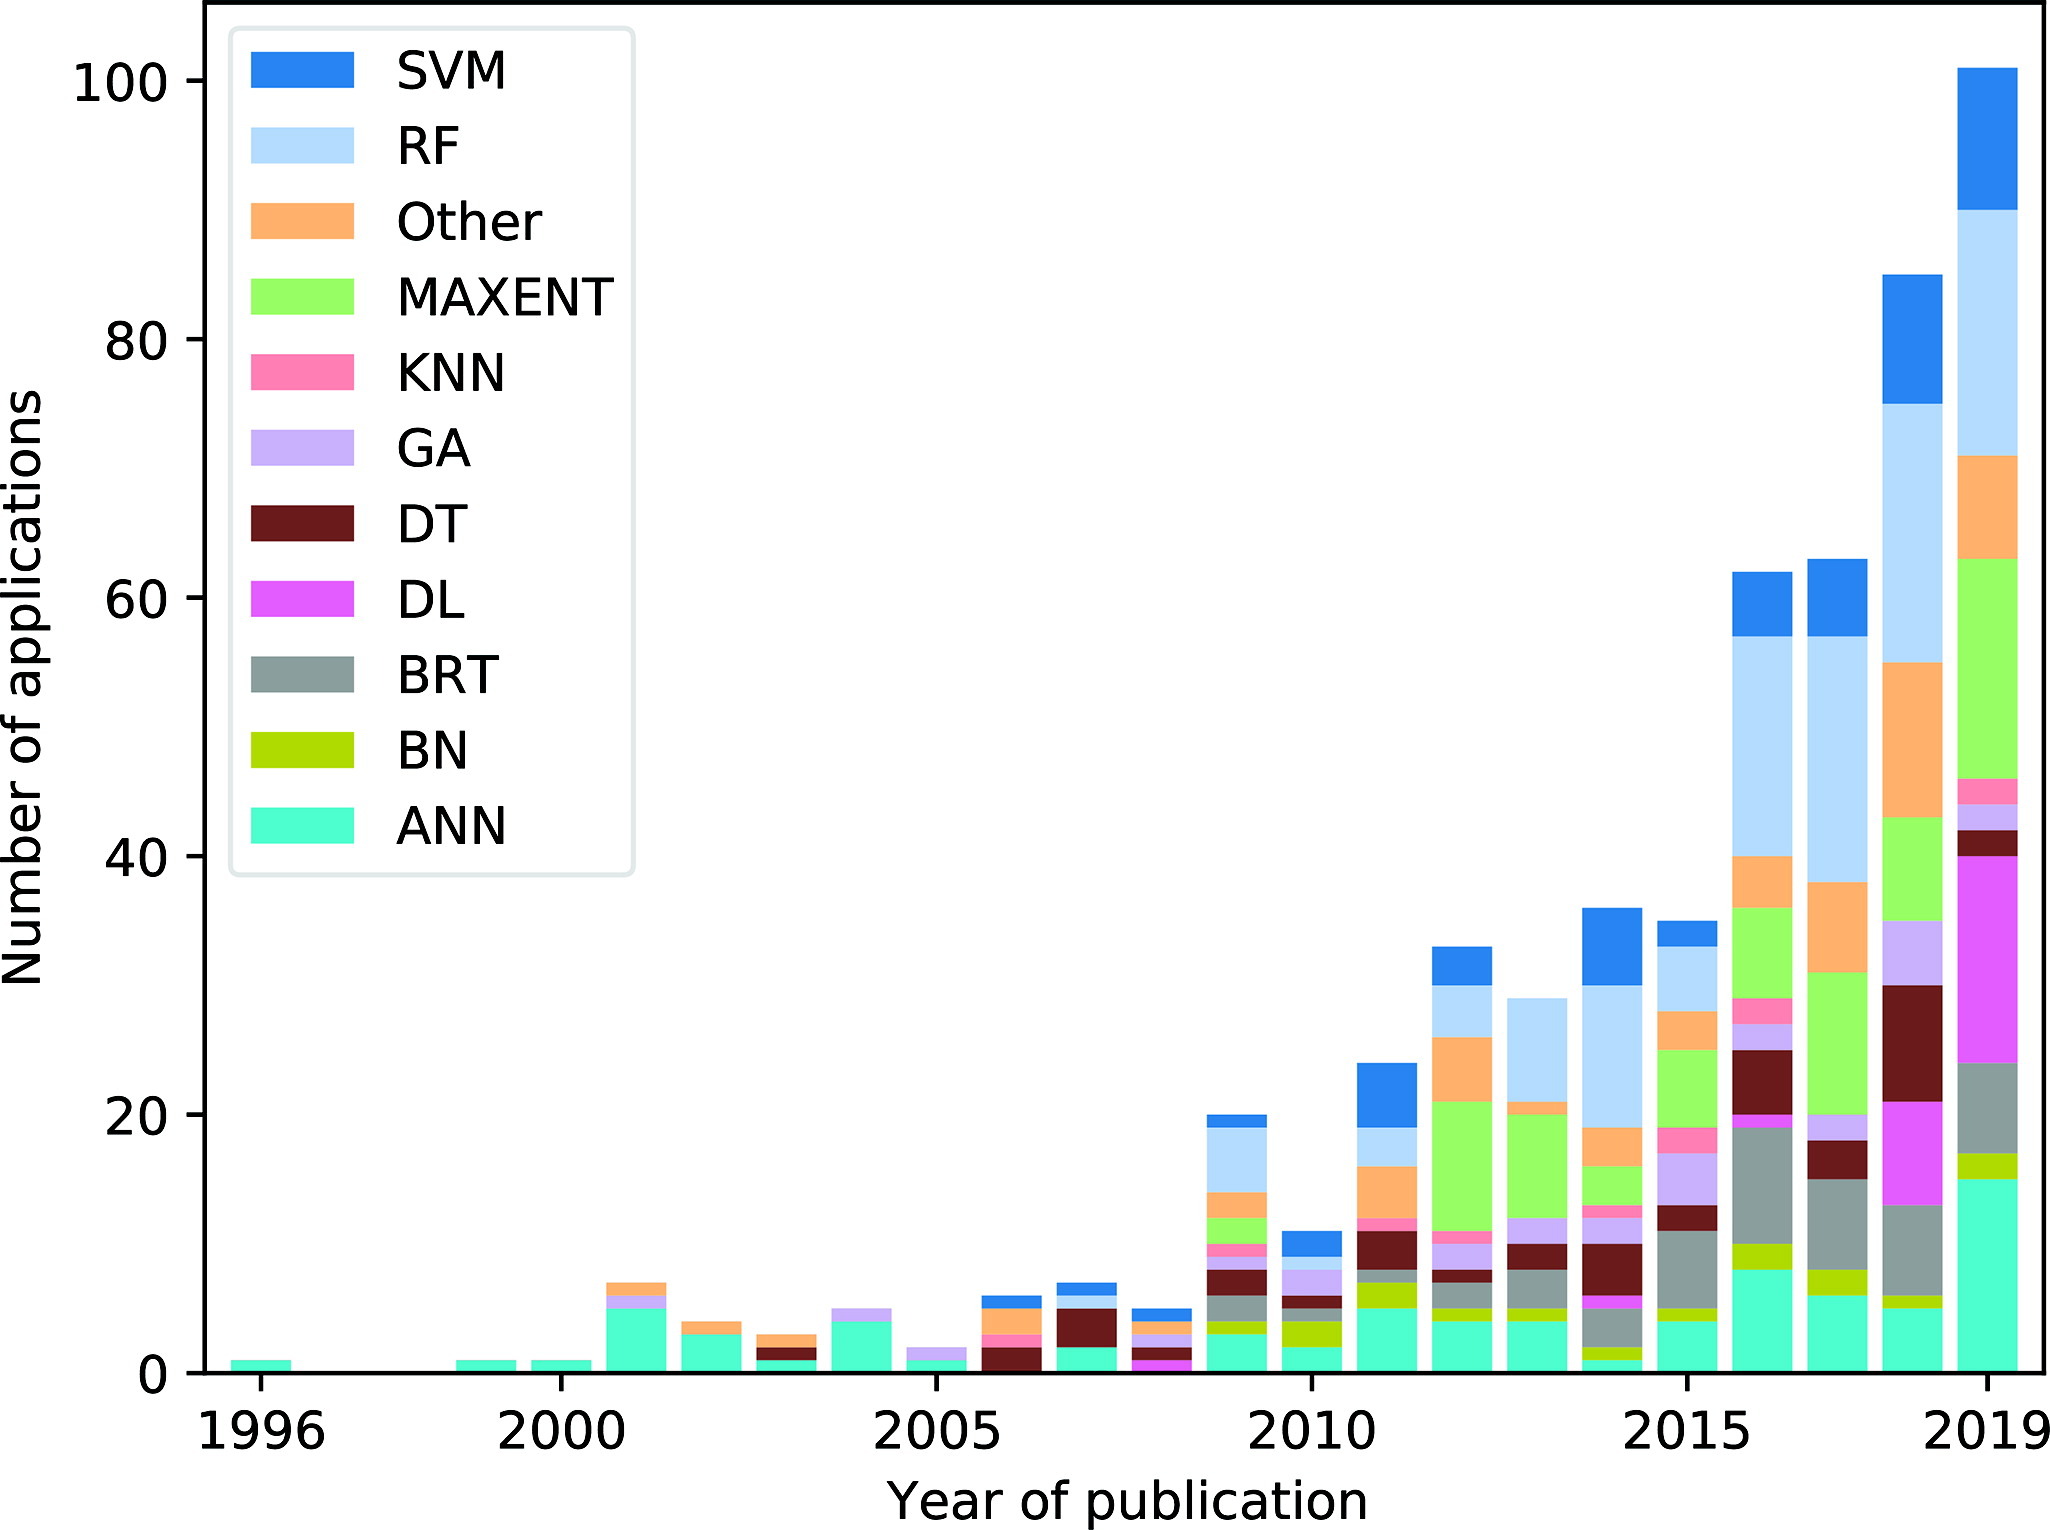
\includegraphics[width=0.6\textwidth]{img/chap1/1-1-ml_wildfire_numbers.jpeg}
    \caption{按类别和年份划分机器学习（ML）应用在野火科学领域的论文数量，引用自\cite{jain2020review}}
    \label{fig:ml_wildfire_numbers}
\end{figure}

随着火灾驱动因素相关数据量的日益增加，特别是卫星遥感技术\cite{forkel2017data}的不断发展，极大地促进了深度学习在野火相关领域的应用。目前，已有诸多研究在野火相关领域中引入了机器学习技术\cite{jain2020review}。

\section{深度学习在野火风险时空预测中的应用}
\label{sec:1-deep-learing}
本节将回顾基于深度学习的野火风险预测模型的最新进展。野火风险预测任务可以被分为三大类：时间序列预测、图像语义分割与分类和时空预测。时间序列模型（如RNN、LSTM、门控循环单元以及Transformer）利用一维特征向量来预测野火风险，而语义分割与分类模型（如CNN和Transformer）则使用二维特征图来生成风险预测。用于时空预测的深度学习模型使用通常将以上两种方法进行结合，输入数据既包含时间序列也包含空间数据。下面我们具体介绍图像语义分割与分类和时空预测任务的进展。

\subsection{图像语义分割与分类}
尽管RNNs和Transformer在捕捉序列间学习任务中的时间依赖性方面表现出色，但这些方法主要对单个像素的时间序列数据进行分类。然而，野火不仅受某个特定小范围的条件影响，还受邻近地区的影响。当RNN使用一维数据输入时，图像的空间结构常常丢失\cite{hu2020spatial}。因此，研究者逐渐转向图像语义分割与分类方法，如卷积神经网络（CNN）、图神经网络（GNN）和Transformer，利用影响因素（如燃料、天气）从$t^{'}<t$开始预测时间$t$的野火风险。这些方法依赖于二维图像输入，能够利用野火传播的空间特性。

作为深度学习领域的基础网络，卷积神经网络（Convolutional Neural Network，CNN）通过卷积操作提取局部空间特征，非常适合捕捉野火风险预测所需的空间信息。例如，\textcite{zhang2019forest}采用了修改版的 AlexNet\cite{krizhevsky2012imagenet}，利用中国云南省的年度火点地图和春季平均影响因素，将图像划分为野火易发区域，模型能够在最后一层的卷积神经网络中通过 softmax 映射输出野火风险概率图。在作者的实验中，发现CNN实现了最高的整体准确率，并利用信息增益率方法，分析了各种野火驱动因素的贡献，确定温度、风速和降水量是最具影响力的因素。在此基础上，生成了全球季度野火易感性地图\cite{zhang2021deep}。一些研究采用了更深层的或结构优化的CNN网络。例如，\textcite{oak2024novel}利用VGG16预测加拿大魁北克的野火易感性，\textcite{nur2022creation}应用了一种元启发式优化算法，对美国普卢马斯国家森林中CNN模型的野火易感性图谱进行微调。此外，一些工作开发混合架构或端到端模型处理数据，预测野火蔓延\cite{allaire2021emulation,li2023predicting}。

除了卷积神经网络（CNN），图神经网络（GNN）和 Transformer 等其他图像分割方法也被应用于野火风险预测。与 CNN 相比，GNN 更擅长处理非欧几里得结构的数据\cite{jiang2022modeling}，而 Transformer 的多头自注意力机制在对图像内的长距离语义依赖进行建模时更为有效。

\subsection{时空预测}
\label{sec:1-2-spatiotemporal-prediction}
上述提到的时间序列预测方法和图像分割与分类方法，分别在捕捉时间依赖性和空间依赖性方面各具优势。然而，它们无法同时处理空间与时间数据，也难以捕捉复杂的跨时空交互模式\cite{prapas2021deep}。为了整合空间结构与时间序列数据，许多研究将两者结合，也将野火预测任务转化成时空序列预测任务。本文的任务即属于时空预测，图\ref{fig:1-2-time-space}展示了野火时空预测任务示意图。实现这种结合主要有三种方法：分离式时空建模（separated spatial and temporal modeling）、耦合式时空建模（coupled spatiotemporal modeling），以及空间增强型耦合时空建模（spatially enhanced coupled spatiotemporal modeling）\cite{xu2025deep}。

\begin{figure}[htbp]
    \centering
    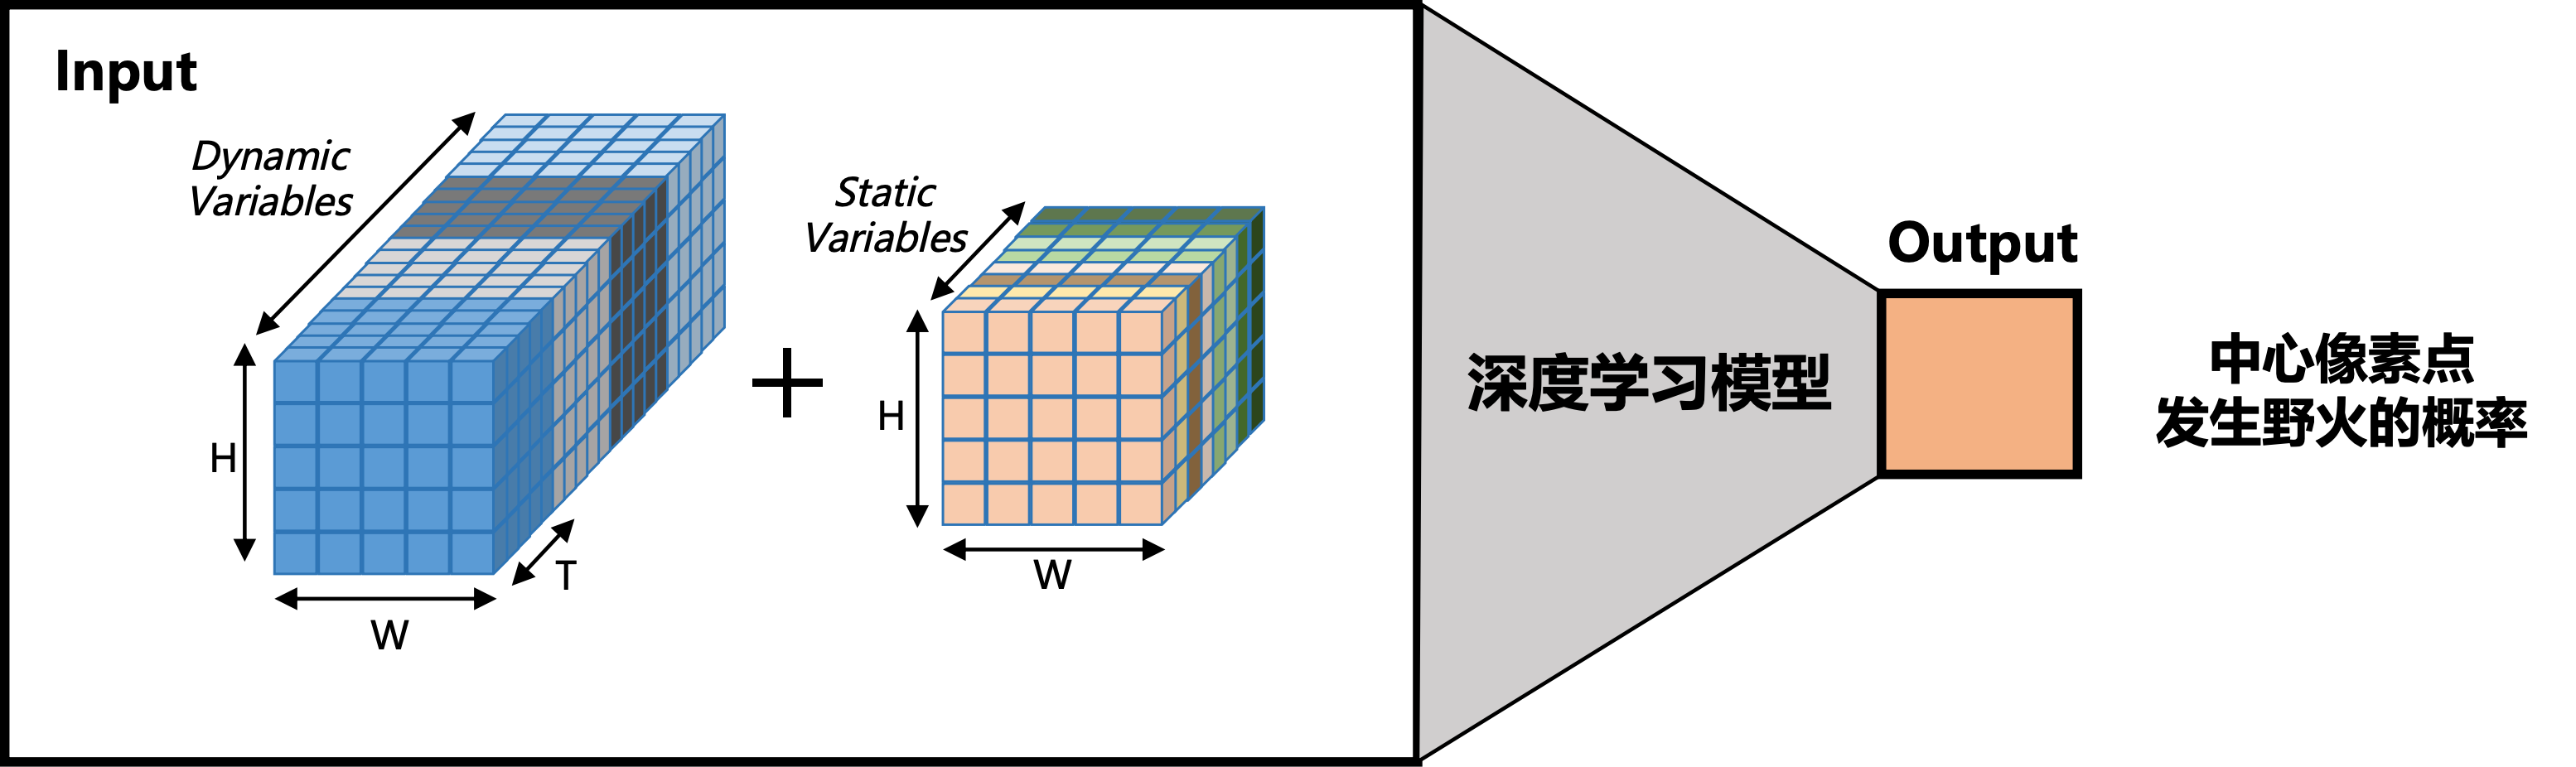
\includegraphics[width=0.9\textwidth]{img/chap1/1-2-time-space.png}
    \caption{野火时空预测任务示意图}
    \label{fig:1-2-time-space}
\end{figure}

具体而言，分离式时空建模是指利用空间建模方法将空间特征抽象为一维特征向量，随后将其输入到时间预测模型中。耦合式时空建模则是将 RNN 中的一维张量转换为三维张量，融入了空间维度，并使用卷积或图结构（而非权重矩阵乘法），基于相邻网格单元当前与过去的状态来决定该网格单元未来的状态。空间增强型耦合时空建模是在正式进入时空建模阶段之前，先引入 CNN 或基于图的方法来提取空间特征\cite{xu2025deep}。

分离式时空建模方法将空间与时间特征的提取分步进行。如图\ref{fig:1-2-separated-modeling}所示，首先在每个时间步上使用卷积神经网络（CNN）等模块对多维空间数据进行特征提取，随后将提取到的二维空间特征降维成一维的全局表征，然后将这些一维向量输入到时间序列模型（如 LSTM 或 GRU）中，以捕捉火灾随时间演变的动态规律，最后通过分类器（或反卷积层映射）输出最终的火灾风险概率。这种范式有效利用了 CNN 在识别复杂空间模式方面的强大能力，又发挥了LSTM或GRU在时间序列建模上的独特优势，从而较好地捕捉野火系统中的时空动态变化\cite{huot2020deep,zhang2022dynamic,marjani2024cnn}。

\begin{figure}[htbp]
    \centering
    \begin{minipage}{0.48\textwidth}
        \centering
        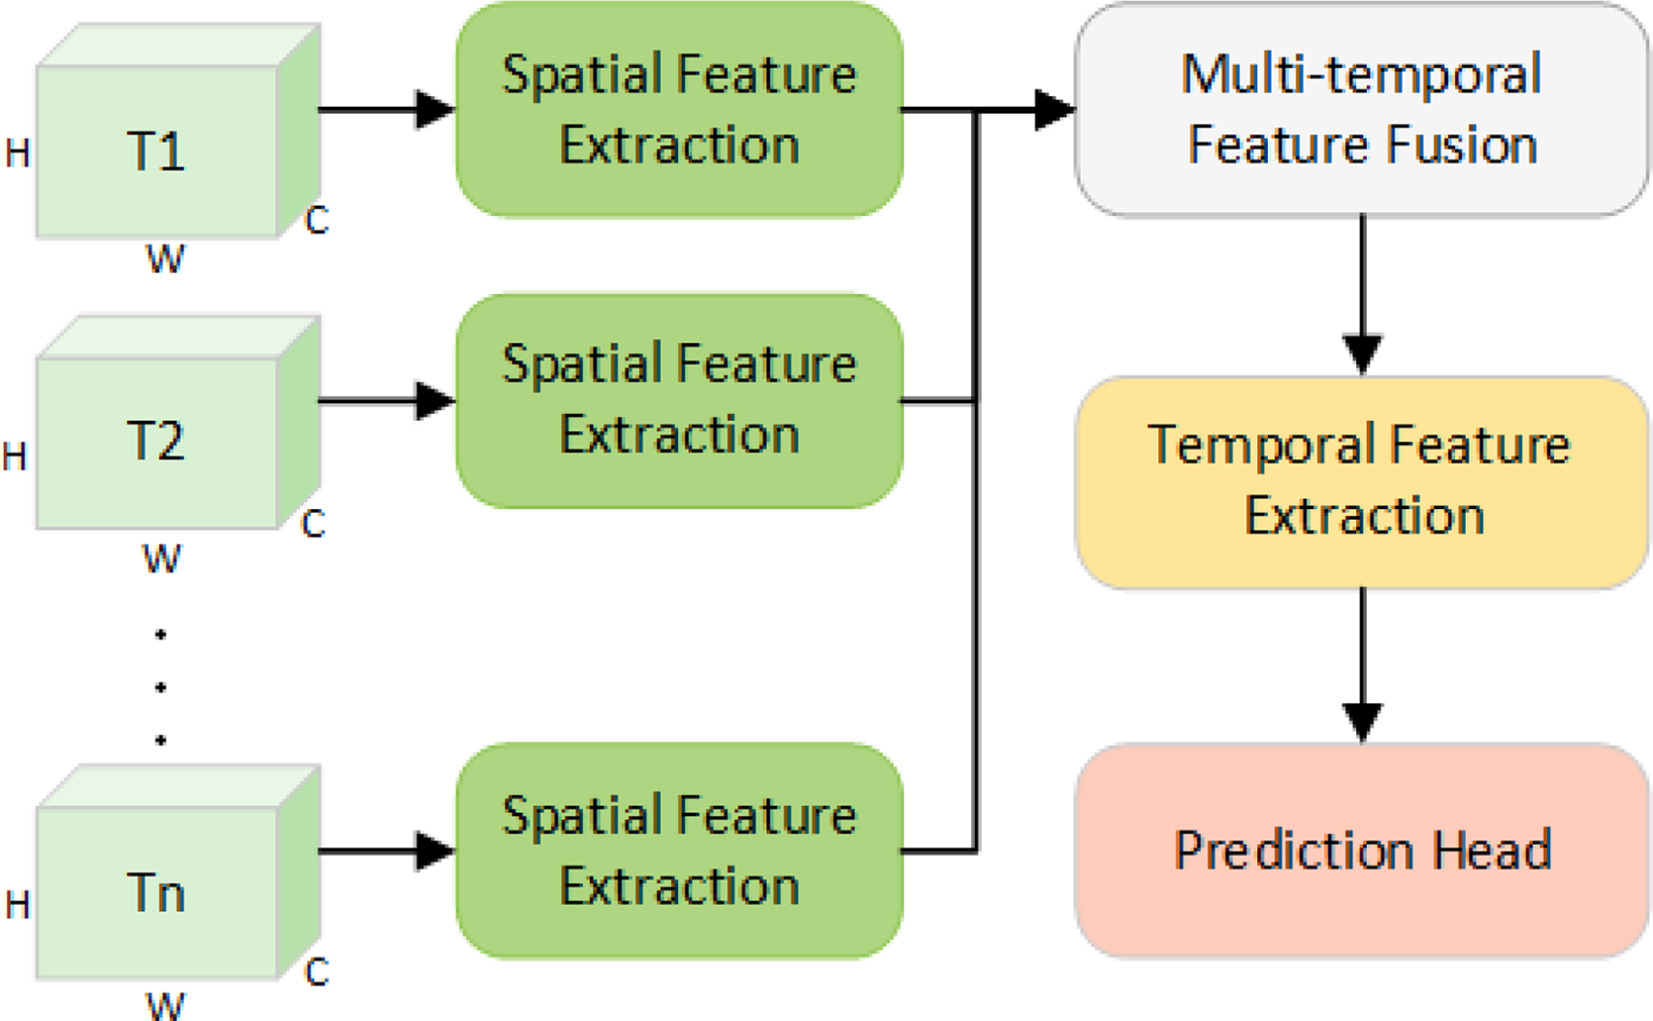
\includegraphics[width=\textwidth]{img/chap1/1-2-separated-modeling.jpg}
        \caption{分离式时空建模示意图，引用自\protect\cite{xu2025deep}}
        \label{fig:1-2-separated-modeling}
    \end{minipage}
    \hfill 
    \begin{minipage}{0.48\textwidth}
        \centering
        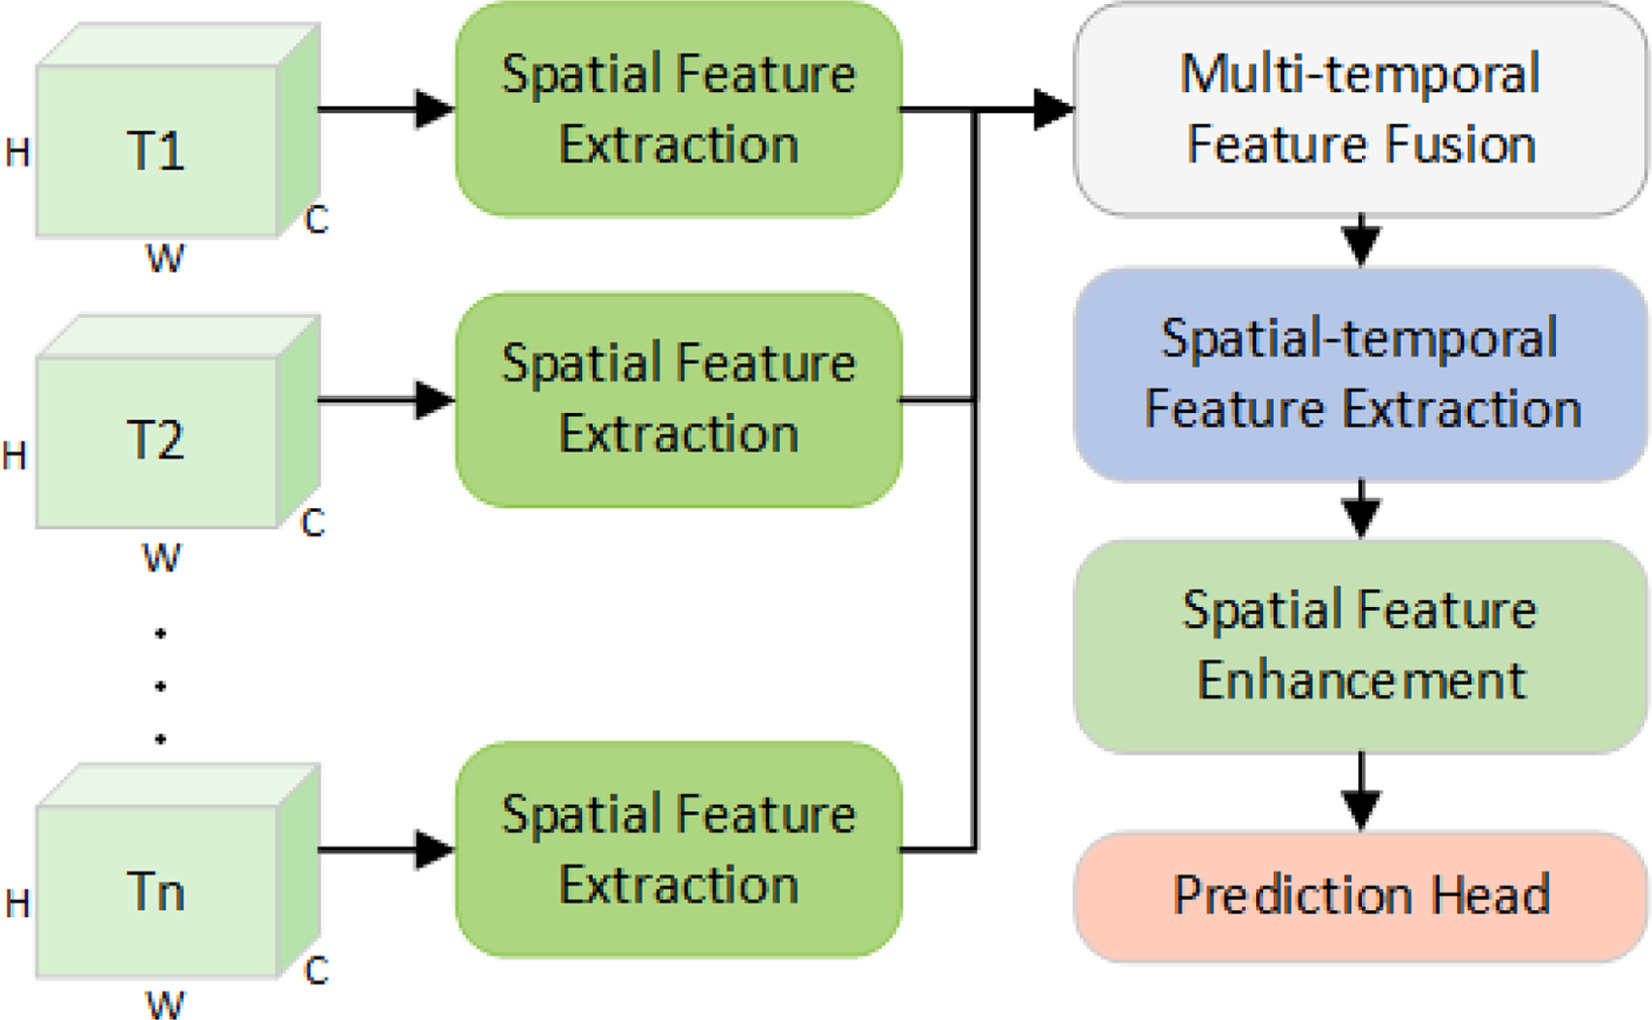
\includegraphics[width=\textwidth]{img/chap1/1-2-spatially-enhanced.jpg}
        \caption{一个典型的空间特征增强型耦合时空野火风险预测模型图，引用自\protect\cite{xu2025deep}}
        \label{fig:1-2-spatially-enhanced}
    \end{minipage}
\end{figure}

视线转向耦合式时空建模，卷积长短期神经网络（ConvLSTM）无疑是被广泛采用的框架。以 \textcite{burge2020convolutional} 的工作为参照，该团队将三组在地形、风场、湿度及植被密度上具有截然不同分布的模拟数据集进行拼合，旨在校验 ConvLSTM 捕捉火情蔓延动态的理论上限。实测反馈极为清晰：该架构的预测准确率直接超越了 CNN 的基准。\textcite{prapas2021deep} 则把研究靶点设在希腊全境的次日火险预警上，他们比较了随机森林模型（RF）、时间序列预测算法（LSTM）、图像分类方法（CNN）以及时空建模方法（ConvLSTM），并得出了几个关键发现。对于 RF 模型，训练数据的构建方式是计算每个空间位置在预测日期前 10 天各个驱动因素的平均值，从而生成维度为 $f\times 1$ 的数据集（其中 $f$ 为驱动因素的数量）。LSTM 模型采用时间序列输入，数据维度为$f\times t$，其中 $t$ 代表时间序列的长度（10天）。对于图像分类任务，空间数据被构建为以目标点为中心的空间图块（patches），其维度为$f\times h\times t$（其中 $h$ 和 $w$ 分别为图像的高度和宽度）。最后，对于使用 ConvLSTM 的时空预测任务，数据集的维度为 $f\times h\times w\times t$。结果表明，LSTM 和 ConvLSTM 的表现优于 RF 和 CNN。在评估二分类结果时，LSTM 总体上优于 ConvLSTM。

空间增强型耦合时空建模在耦合时空建模的基础上，将卷积层与 ConvLSTM 结合，以进一步强化空间特征的提取。如\ref{fig:1-2-spatially-enhanced}所示，在将数据送入时间模型（如 ConvLSTM）之前，会先进行降维处理。与分离式时空建模方法相比，这种方法在整个建模过程中往往能保留一定程度的空间信息，从而在最终的预测结果中，能够保留更精细的空间模式\cite{xu2025deep,ji2024global,he2024deep}。

本节回顾了应用于野火风险预测的深度学习方法的最新进展，重点关注其从时间、空间建模向时空序列建模的演进。得益于其优秀的架构，深度学习模型在捕捉非线性关系方面表现出色，能够对高维时空数据中复杂的关系进行建模，包括气象变量、植被指数、地形特征和社会因素等，从而更好地实现对野火风险的预测。

\section{本论文主要内容及结构}
\label{sec:denotation}
本论文除附录外共分为六个章节。第一章为引言，阐述研究背景与意义，并综述深度学习模型在野火风险预测领域的应用。第二章详细介绍FireCube数据集，包括区域概况及时空数据构建，采样方式及训练数据，特征变量分析。第三章阐述基于Swin Transformer的架构设计，包括气象动力学特征提取模块，静态地貌特征编码模块，特征融合模块以及物理信息启发的数据重构与注意力偏置。第四章展示实验结果与评估，包括模型训练，实验设置与性能对比，消融实验等。第五章为可解释性分析部分，重点阐述基于SHAP的归因分析和交叉注意力融合机制分析。第六章为总结与讨论，对本研究进行总结，并指出局限性和未来展望。附录详细介绍了研究中使用的算法等。

    \chapter{FireCube数据集及变量分析}
\label{chap:dataset}
有一些公开的数据集可以用于野火风险预测，但它们在解决的任务、观测变量、空间和时间分辨率上存在显著差异。本文选择FireCube数据集作为使用的数据集，它由 Prapas 发布\cite{prapas2021deep}、Kondylatos 扩展与改进\cite{kondylatos2022wildfire}，并最终由\textcite{prapas2022firecube}分类整理为 2D 和 3D 格式，可在zenodo网站\cite{prapas2022firecube_dataset}得到。观测变量包括气象数据、卫星衍生数据、地形特征、人类相关活动以及历史火灾记录。此外，还提供了土地覆盖类型（CLC）和火险指数（FWI）。任务目标是预测每个像素的野火是否会在第二天燃起并扩大规模，该任务相当于对每一个像素点的二元分类任务，判断该像素点是否发生野火事件。

\section{区域概况及时空数据构建}
\label{sec:regional-overview-and-spatio-temporal-data-construction}
FireCube数据集定义了一个像素级别的野火预测任务，包含了从2009年至2021年间90个变量的多变量时空数据流，分辨率为$1km\times 1km\times 1day$。我们选择FireCube数据集，其以希腊作为研究地点。因为希腊展现出独特的野火模式和环境特征，使其成为野火预测和驱动因素的理想案例研究。希腊位于地中海气候区，夏季炎热干燥，极易发生野火。此外，其复杂的地形、植被分布以及人类活动的影响进一步加剧了野火风险和破坏性。数据集所定义的区域面积为$1253km\times 983km$，包括希腊及东地中海部分地区。

野火数据来源于 EFFIS 的历史过火面积数据\cite{san2013european}以及 MODIS 的活跃火点产品\cite{giglio2016collection}。该数据集对这两类数据进行了空间交叉（spatial intersection）分析，以重建火灾的起火日期。通过将活跃火点与过火面积相互关联，确定了每场野火的起火日期，并将属于同一野火事件的燃烧面积进行合并。为了确定起火日期，研究会在燃烧面积的矢量数据周围创建一个 1 公里的缓冲区，并在此缓冲区内，搜索在 EFFIS 记录的起火日期前一周内所生成的活跃火点。

\section{采样方式及训练数据}
\label{sec:sampling-method-and-training-data}
由于野火风险预测本质上是一项不平衡分类任务，其中正样本的数量远少于负样本，因此为了便于模型训练，需要对原始数据进行采样，构建训练样本，并划分训练集，验证集，测试集。研究\cite{kondylatos2022wildfire}的作者按照如下方式提取样本：对于目标日$T+1$，对于目标像素$1km\times 1km$的格点，静态变量形成一个以目标像素为中心的$25km\times 25km$的斑块；动态变量由从$T-9$天到$T$的$25km\times 25km\times 10day$时间序列组成。每个样本均包含数个静态变量与动态变量，因此本任务本质上属于前文第\ref{sec:1-2-spatiotemporal-prediction}节中所述的时空预测问题。其中正样本代表该目标像素点发生野火事件，负样本代表该目标像素点未发生野火事件。对于每个正样本，会从不同地点抽取少量负样本，负样本有两种来源，一是随机抽取，二是从与正样本土地覆盖类型相似的地区抽样，以提高任务难度。

图\ref{fig:2-2-samples}展示了数据集中各年份正负样本的数量分布。总体而言，2009年至2020年间的样本总量保持相对均衡，然而，2021年的数据量出现了显著的激增。这一异常增长主要归因于2021年夏季在希腊地区爆发的规模空前、破坏力极强的极端野火事件\cite{giannaros2022meteorological}。总体数据包括71471个训练样本，其中包含13518个正样本和57953个负样本，来自2009年-2018年的原始数据；6430个验证样本，其中包含1300个正样本和5130个负样本，均来自2019年；42820个测试样本，其中包含2020年的1228个正样本、4860个负样本和2021年4407个正样本、32325个负样本。训练样本、验证样本和测试样本构成模型训练评估时的训练集，验证集，测试集。提取的训练数据可在\cite{prapas2022training}中获取。在深度学习理论中，训练集是用于模型内部参数（Parameters）估计或学习的数据样本集合，验证集是用于模型选择和超参数调优（Hyperparameter Tuning）的数据样本集合，测试集是用于对最终选定的最优模型进行泛化误差估计的数据样本集合\cite{bengio2017deep}。
\begin{figure}[htbp]
    \centering
    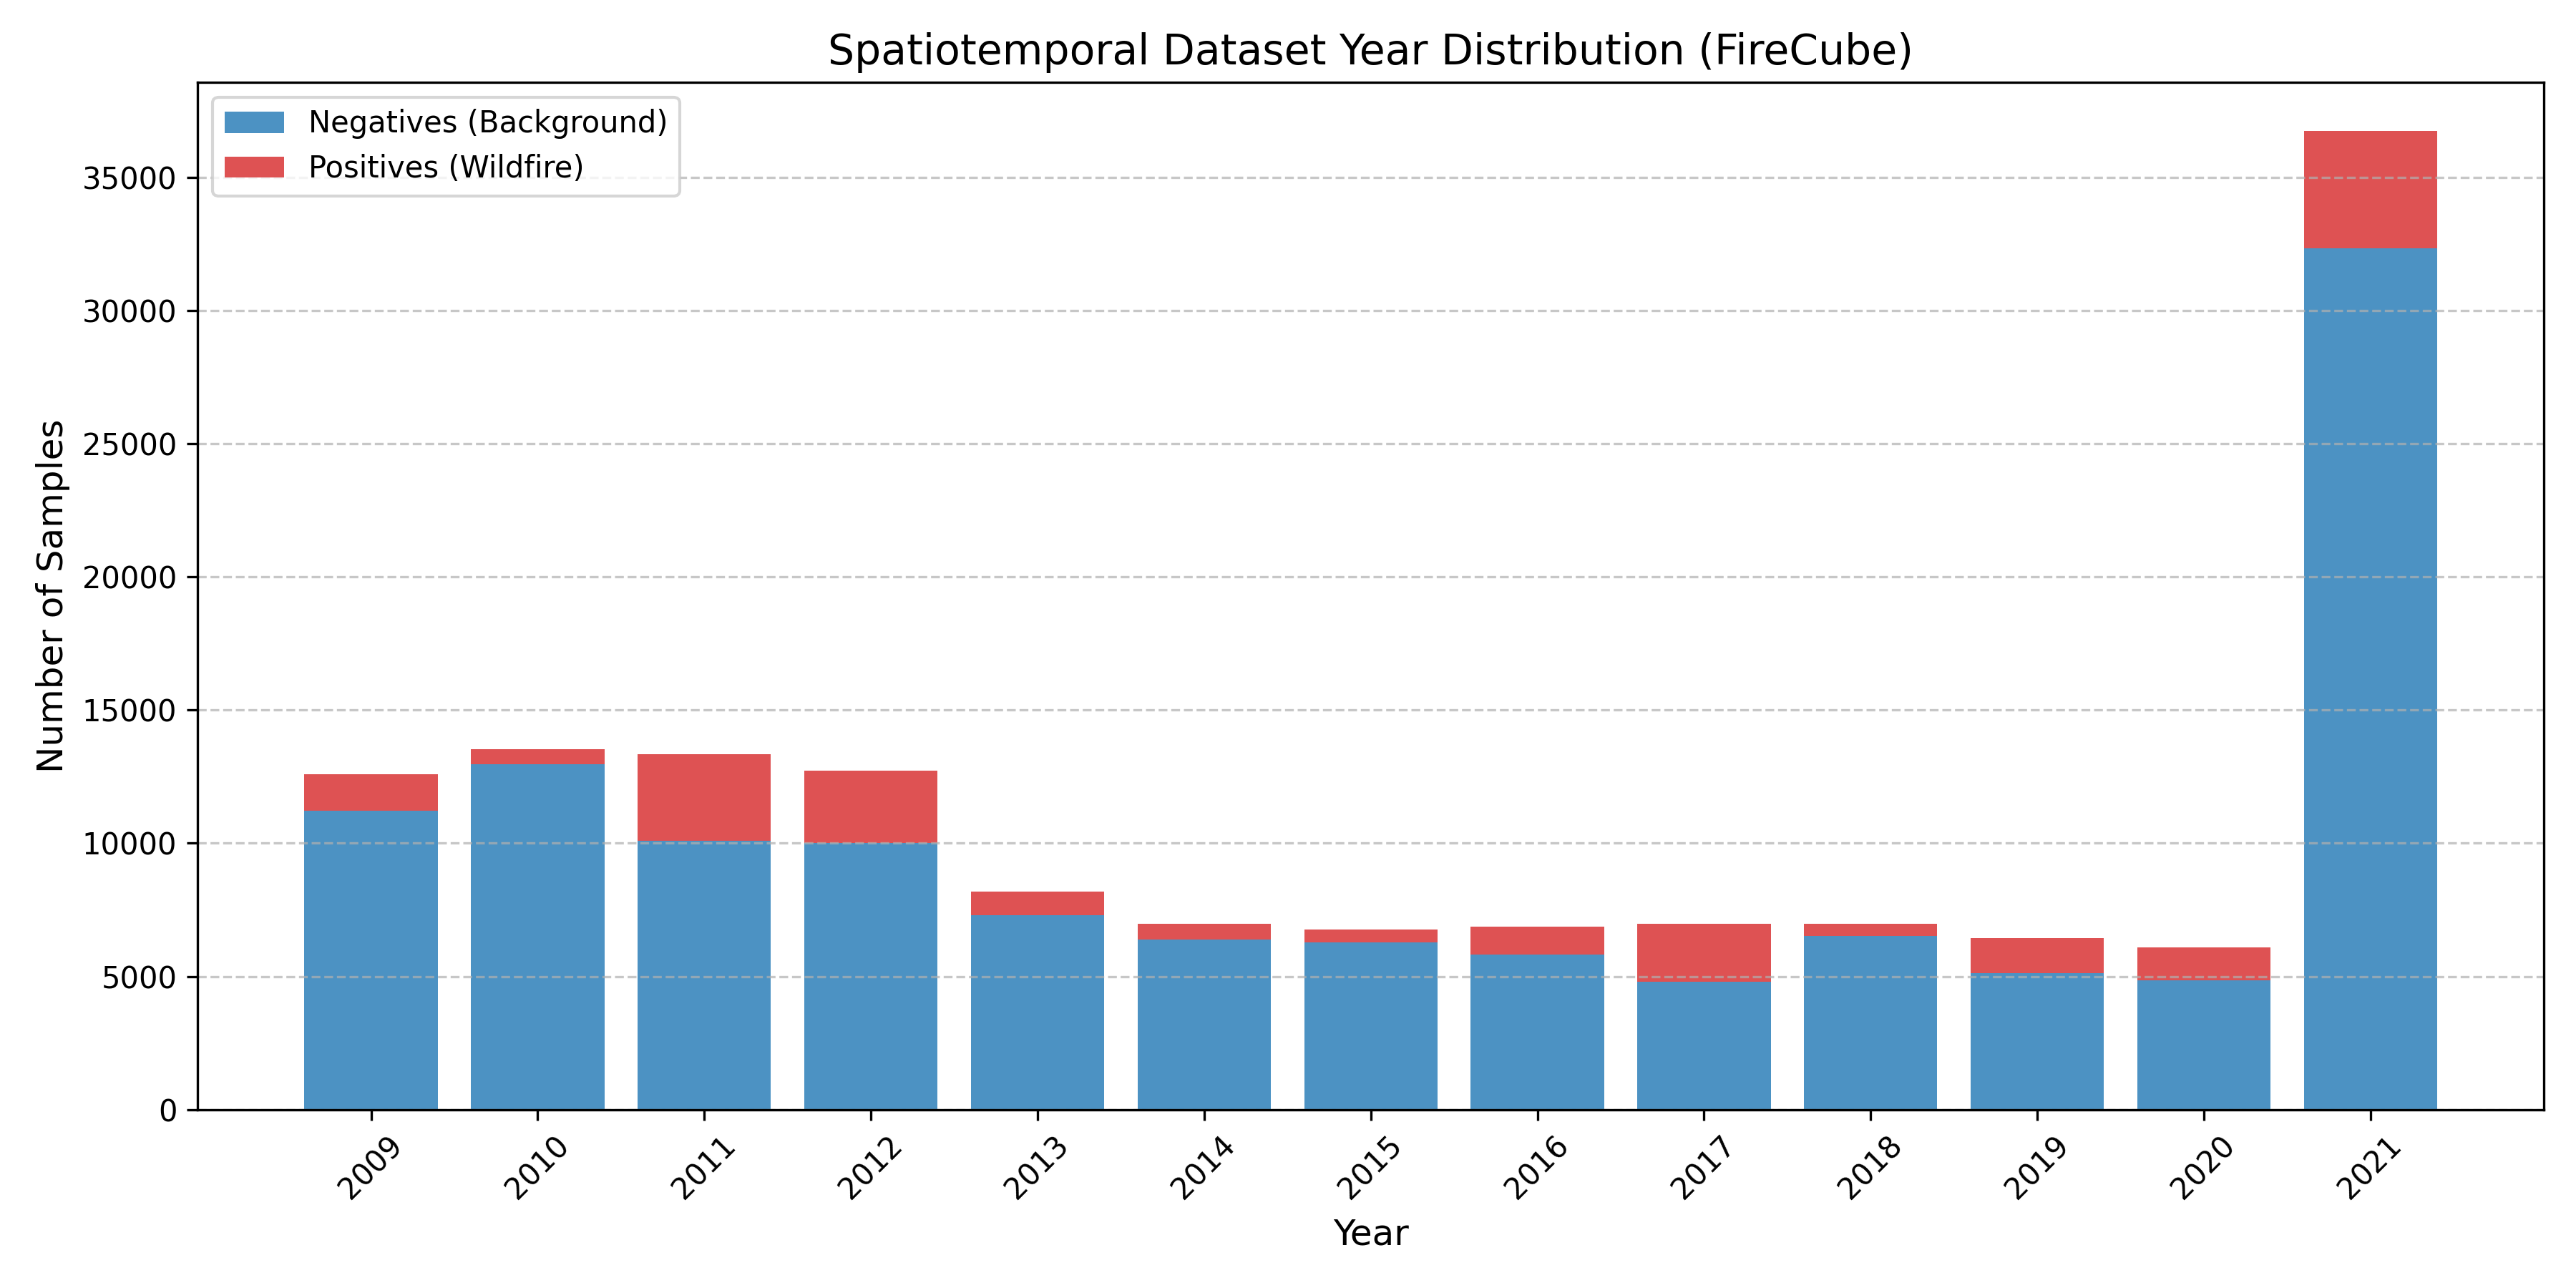
\includegraphics[width=0.9\textwidth]{img/chap2/2-2-samples.png}
    \caption{FireCube训练数据中各年份采样的样本数量}
    \label{fig:2-2-samples}
\end{figure}

同时，原始数据集虽然包含了90个变量，但其中存在大量的时间切片冗余，如不同年份的的静态背景数据以及统计维度的相似性（如同一气象指标的最高、最低和平均值），为了降低模型复杂度，避免维度灾难以及共线性带来的过拟合问题，FireCube数据集对原始变量进行整合和缩减，最终保留了25个变量，其中包含15个静态变量和10个动态变量。表\ref{tab:static_vars}展示了数据集静态特征变量列表，分别包含地形特征、水文与人类活动和地表覆盖变量三个大类，其中地表覆盖变量采用one-hot独热编码，详细的地表覆盖类型及物理含义如表\ref{tab:clc_vars}所示。

\begin{table}[htbp]
    \centering
    \caption{FireCube 数据集静态特征变量列表}
    \label{tab:static_vars}
    \renewcommand{\arraystretch}{1.5} 
    \begin{tabularx}{\textwidth}{
        >{\raggedright\arraybackslash}p{2.8cm} 
        >{\raggedright\arraybackslash}p{4.5cm} 
        >{\raggedright\arraybackslash}p{2.5cm} 
        >{\raggedright\arraybackslash}X }
        \toprule
        \textbf{变量大类} & \textbf{变量名称} & \textbf{中文名称} & \textbf{物理含义} \\
        \midrule
        
        \textbf{地形特征} 
        & Digital elevation model (DEM) & 数字高程模型 & 表征海拔高度，影响局地气候与植被的垂直分布 \\
        & Slope & 坡度 & 影响野火蔓延的动力学特征 \\
        \midrule
        
        \textbf{水文与人类活动} 
        & Distance to waterway & 与水域的距离 & 反映地表可用水源分布及天然防火隔离带的邻近程度 \\
        & Distance to roads & 与道路的距离 & 衡量人类活动的可达性与基础设施分布 \\
        & Population density & 人口密度 & 表征区域人口聚集度，反映人类活动对自然环境的干扰强度 \\
        \midrule
        
        \textbf{地表覆盖变量}
        & 10 Copernicus Corine Land Cover variables & 10 类地表覆盖类型 & 表征地表可燃物类型与空间分布基底（包含森林、灌木、人造表面等10个具体子类，详见表 \ref{tab:clc_vars}） \\
        
        \bottomrule
    \end{tabularx}
\end{table}


\begin{table}[htbp]
    \centering
    \caption{FireCube 数据集地表覆盖变量 (CLC) 详细分类}
    \label{tab:clc_vars}
    \renewcommand{\arraystretch}{1.5} 
    % CLC 表格同样采用顶部对齐
    \begin{tabularx}{\textwidth}{ 
        >{\raggedright\arraybackslash}p{4.2cm} 
        >{\raggedright\arraybackslash}p{3cm} 
        >{\raggedright\arraybackslash}X }
        \toprule
        \textbf{变量名称} & \textbf{中文名称} & \textbf{物理含义} \\
        \midrule
        
        Artificial ground & 人造表面 & 连续的城市结构、工业或商业单元、公路和铁路网络及相关土地、港口区域、机场、矿产开采场、垃圾场、建筑工地、城市绿地、体育和休闲设施 \\
        \midrule
        
        Discontinuous urban fabric & 城市不连续表面 & 不连续的城市，如城镇边缘、绿化带等 \\
        \midrule
        
        Arable land & 可耕种地 & 非灌溉耕地、永久灌溉土地、稻田 \\
        \midrule
        
        Permanent crops & 永久耕地 & 果园、葡萄园等农业用地 \\
        \midrule
        
        Pastures & 牧场 & 牧场、天然或人工草地 \\
        \midrule
        
        General agriculture & 普通农用地 & 与永久作物相关的一年生作物、复杂种植模式的作物、大面积自然植被覆盖的主要用于农业的土地 \\
        \midrule
        
        Forests & 森林 & 阔叶林、针叶林、混交林 \\
        \midrule
        
        Miscellaneous vegetation & 植被杂项 & 自然草地、荒原、硬叶植被、过渡林和灌木 \\
        \midrule
        
        Miscellaneous without vegetation & 无植被杂项 & 沙地、裸岩、极稀疏植被、烧毁区域、冰川、全年积雪区域 \\
        \midrule
        
        Water & 水体 & 内陆沼泽、泥炭沼泽、盐沼、潮间带泥滩、沿海泻湖、河口、海洋和湖泊 \\
        \bottomrule
    \end{tabularx}
\end{table}

表\ref{tab:dynamic_vars}展示了FireCube 数据集动态特征变量列表，包含气温与热力、湿度与降水、空气动力与气压、植被与土壤四个大类的特征变量。值得一提的是，虽然\textcite{prapas2022training}构造的训练数据包含25个特征变量，但其余变量依然在数据集中，只是没有被选择输入到深度学习神经网络中，例如原始数据中包含最大经向风速（$max\_wind\_v10$）和最大纬向风速（$max\_wind\_u10$），而作者选择保留了最大风速（$max\_wind\_speed$）作为输入。但是，我们可以从经向风速和纬向风速中提取出风向的信息，从而对野火蔓延预测提供指导，因此，在后续进行改进与分析时可能会使用更多特征变量。

\begin{table}[htbp]
    \centering
    \caption{FireCube 数据集动态特征变量列表}
    \label{tab:dynamic_vars}
    % 拉大行高，保持呼吸感
    \renewcommand{\arraystretch}{1.5} 
    % 全部改用 p 列（顶部对齐），加入 \raggedright 防止文字被强行拉伸溢出
    \begin{tabularx}{\textwidth}{
        >{\raggedright\arraybackslash}p{2.8cm} 
        >{\raggedright\arraybackslash}p{4.5cm} 
        >{\raggedright\arraybackslash}p{2.5cm} 
        >{\raggedright\arraybackslash}X }
        \toprule
        \textbf{变量大类} & \textbf{变量名称} & \textbf{中文名称} & \textbf{物理含义} \\
        \midrule
        
        \textbf{气温与热力} 
        & Maximum 2m temperature & 2m最高温度 & 表征大气最热时段的热力学状态 \\
        & Day land surface temperature & 日间地表温度 & 卫星反演的白天陆地表面温度 \\
        & Night land surface temperature & 夜间地表温度 & 卫星反演的夜间陆地表面温度 \\
        \midrule
        
        \textbf{湿度与降水} 
        & Maximum 2 m dew point temperature & 2m最高露点温度 & 反映近地表空气中的绝对水汽含量 \\
        & Minimum relative humidity & 最小相对湿度 & 表征空气的极端干燥程度\\
        & Total precipitation & 日总降水量 & 反映地表水分补充情况\\
        \midrule
        
        \textbf{空气动力与气压} 
        & Maximum wind speed & 最大风速 & 影响野火推进速率与方向 \\
        & Maximum surface pressure & 最高表面气压 & 反映大尺度天气系统的状态 \\
        \midrule
        
        \textbf{植被与土壤} 
        & Normalized difference vegetation index (NDVI) & 归一化植被指数 & 反映植被覆盖度与生长活力，表征地表可燃物的现存状态 \\
        & Soil moisture index (sminx) & 土壤湿度指数 & 衡量地表及浅层土壤的干旱缺水程度 \\
        
        \bottomrule
    \end{tabularx}
\end{table}

\section{特征变量分析}
\label{sec:characteristic-variable-analysis}
本节通过探索性数据分析（Exploratory Data Analysis，EDA）揭示野火发生与环境因子之间的内在联系，为模型的设计提供依据。
\subsection{静态变量分析}
\label{sec:static-variables-analysis}
图\ref{fig:2-3-monthly-distribution}展示了研究区域内野火发生频次的月度分布情况。从图中可以清晰地观察到，野火的发生呈现出极强的季节性聚集特征。全年绝大多数的火灾集中爆发在夏季和初秋，其中 8月份 是火灾风险的绝对高峰期，单月发生频次占到了总样本的 56.0\%，紧随其后的是 7月（22.8\%）和 9月（11.1\%）。这三个月累计贡献了全年近 90\% 的火灾事件。相反，在 11月至次年 5月的冬春季节，火灾发生率极低，各月占比均不足 1\%。

\begin{figure}[H]
    \centering
    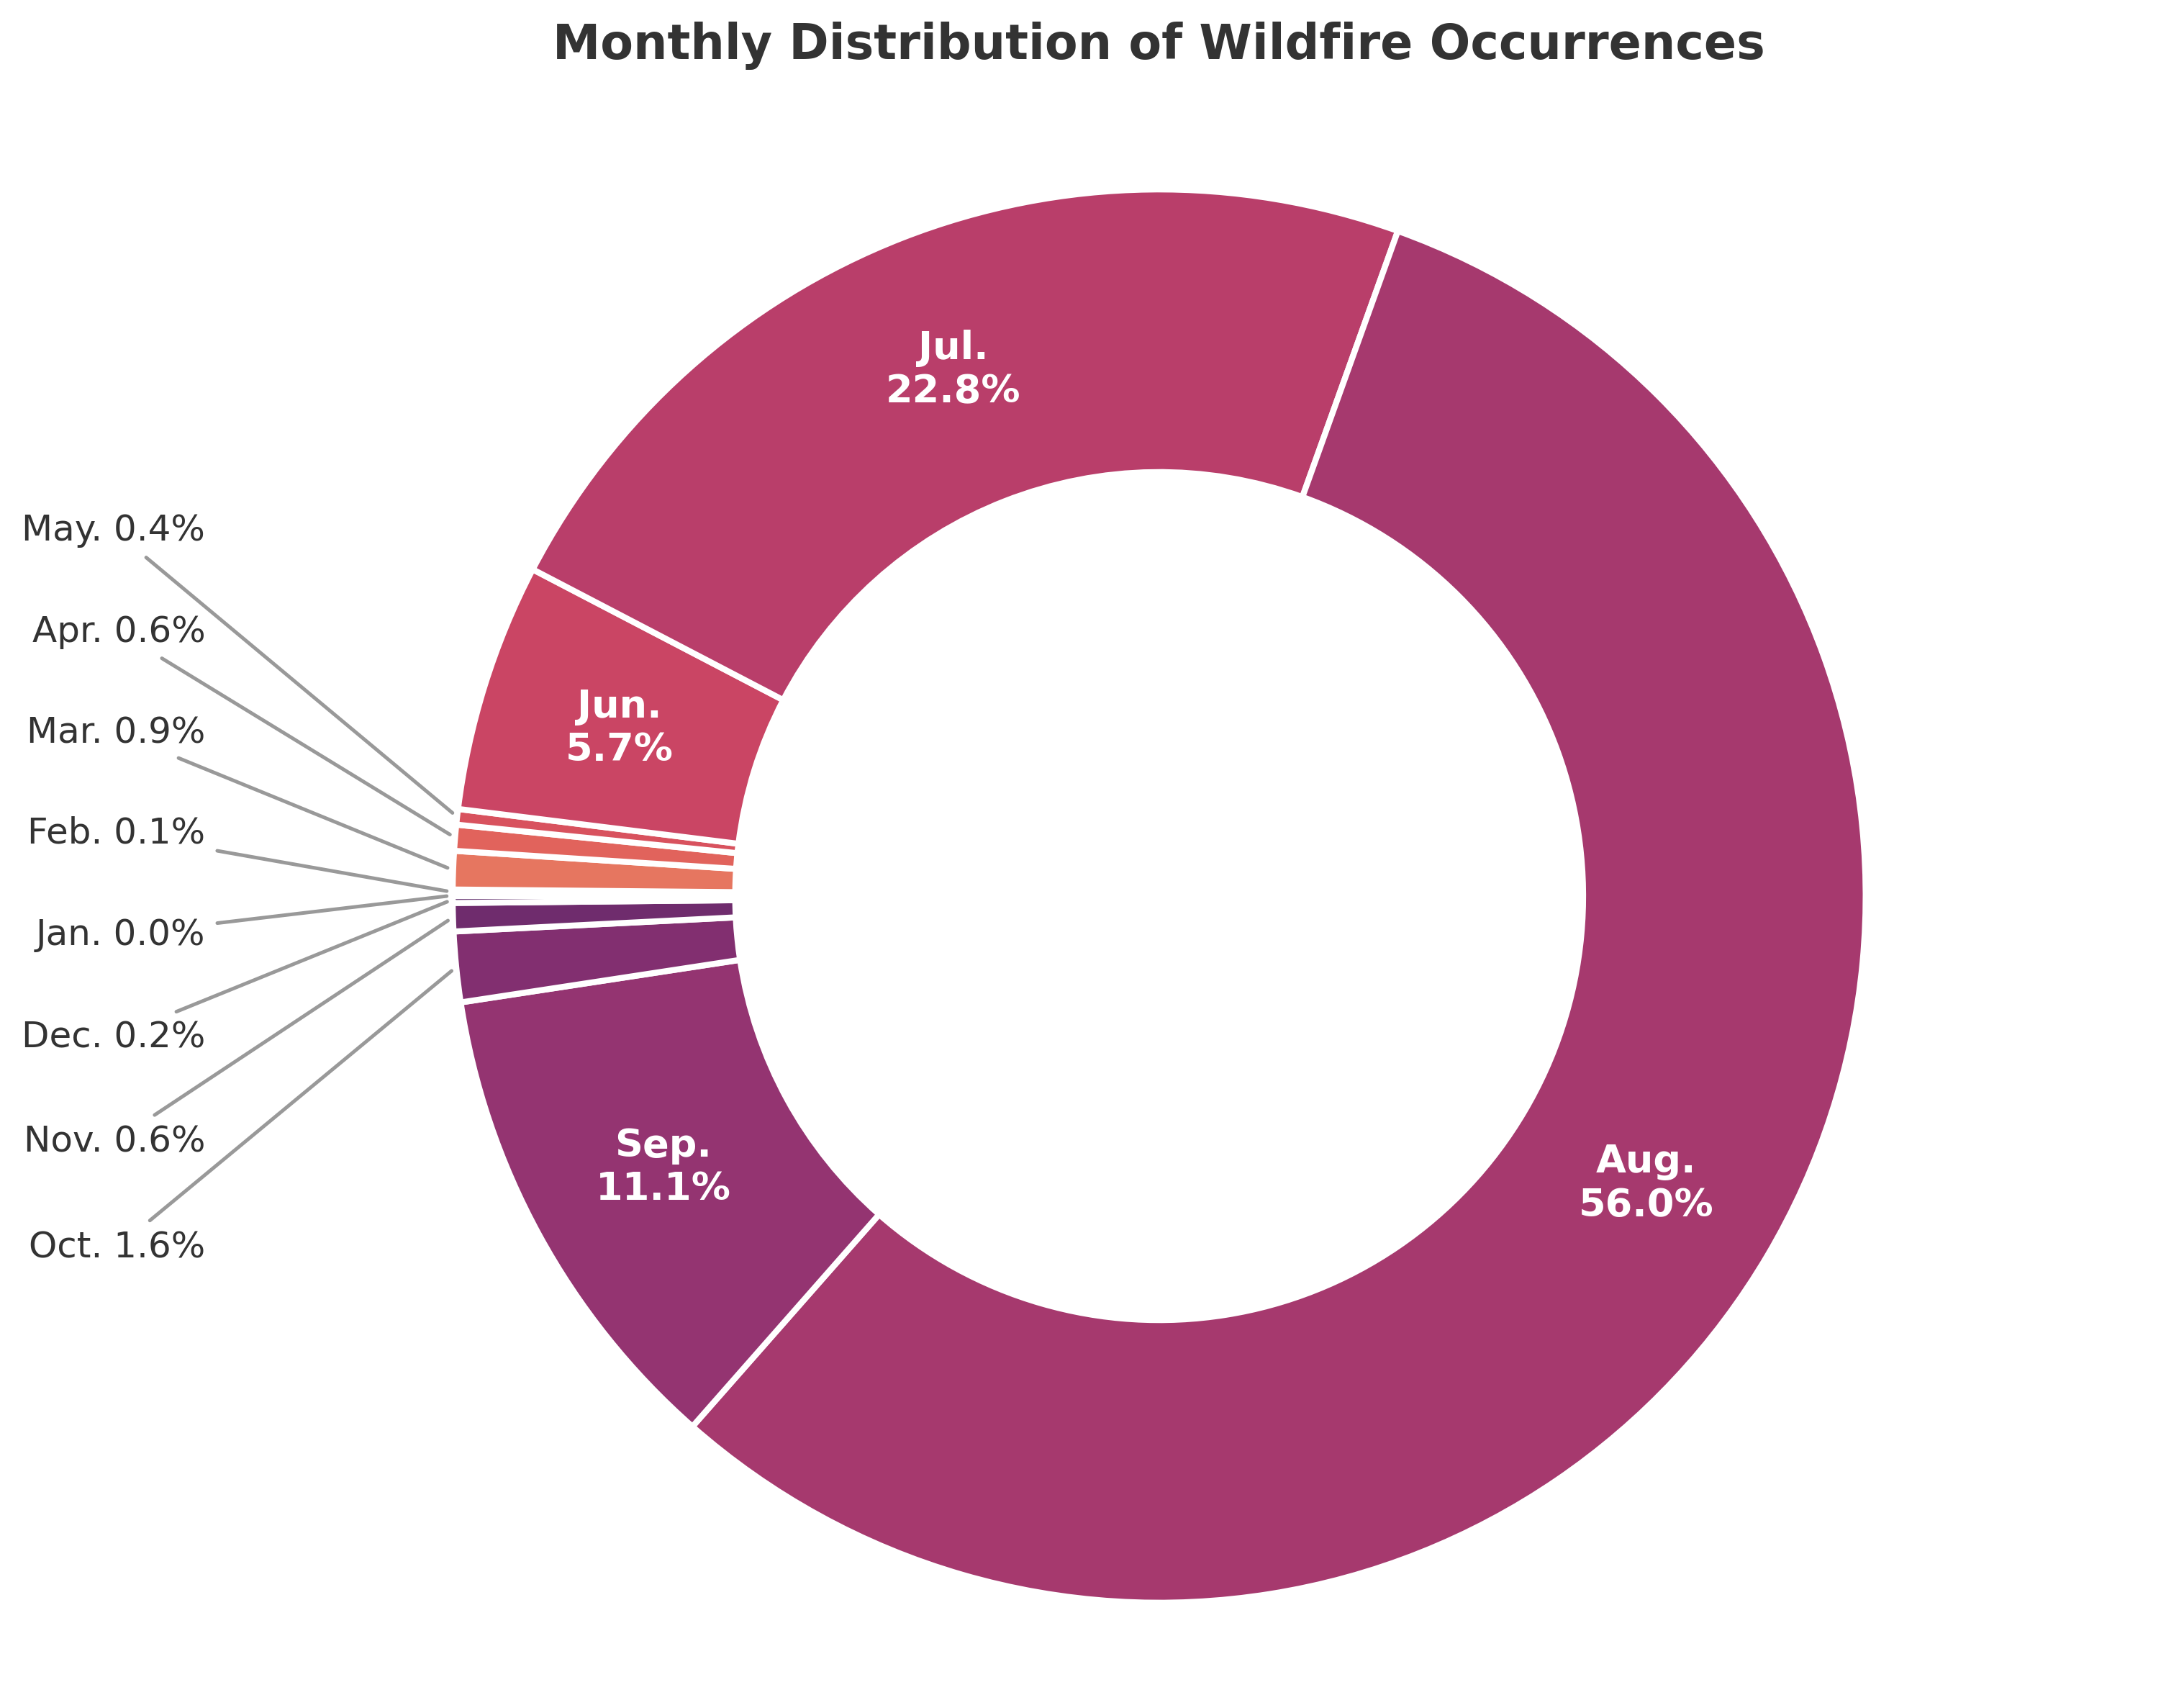
\includegraphics[width=0.9\textwidth]{img/chap2/2-3-monthly-distribution.png}
    \caption{FireCube数据集中野火发生频次的月度分布}
    \label{fig:2-3-monthly-distribution}
\end{figure}

这种极端的分布规律与该地区典型的地中海气候高度吻合。盛夏时期受副热带高压控制，持续的高温与稀少的降水导致地表植被含水量急剧下降，形成了极其易燃的环境，而冬春季节受西风带影响，降水充沛，环境湿度大，有效抑制了火灾的发生。

图\ref{fig:2-3-clc}展示了野火在不同 Corine 土地覆盖 （CLC）类型上的空间分布规律。从统计结果可以清晰地看到，野火的发生地点具有极强的植被选择性。其中，植被杂项（Miscellaneous vegetation）是火灾最密集的区域，其正样本数量以绝对优势位居第一，说明火灾易发生在混合植被与灌木草地，也说明该区域此种土地覆盖类型可能较多；其次是森林（Forests）与普通农用地（General agriculture）。相对而言，城市不连续表面（Discontinuous urban fabric）、人造表面（Artificial ground）以及无植被杂项（Miscellaneous without vegetation）发生火灾的频次极低。

\begin{figure}[htbp]
    \centering
    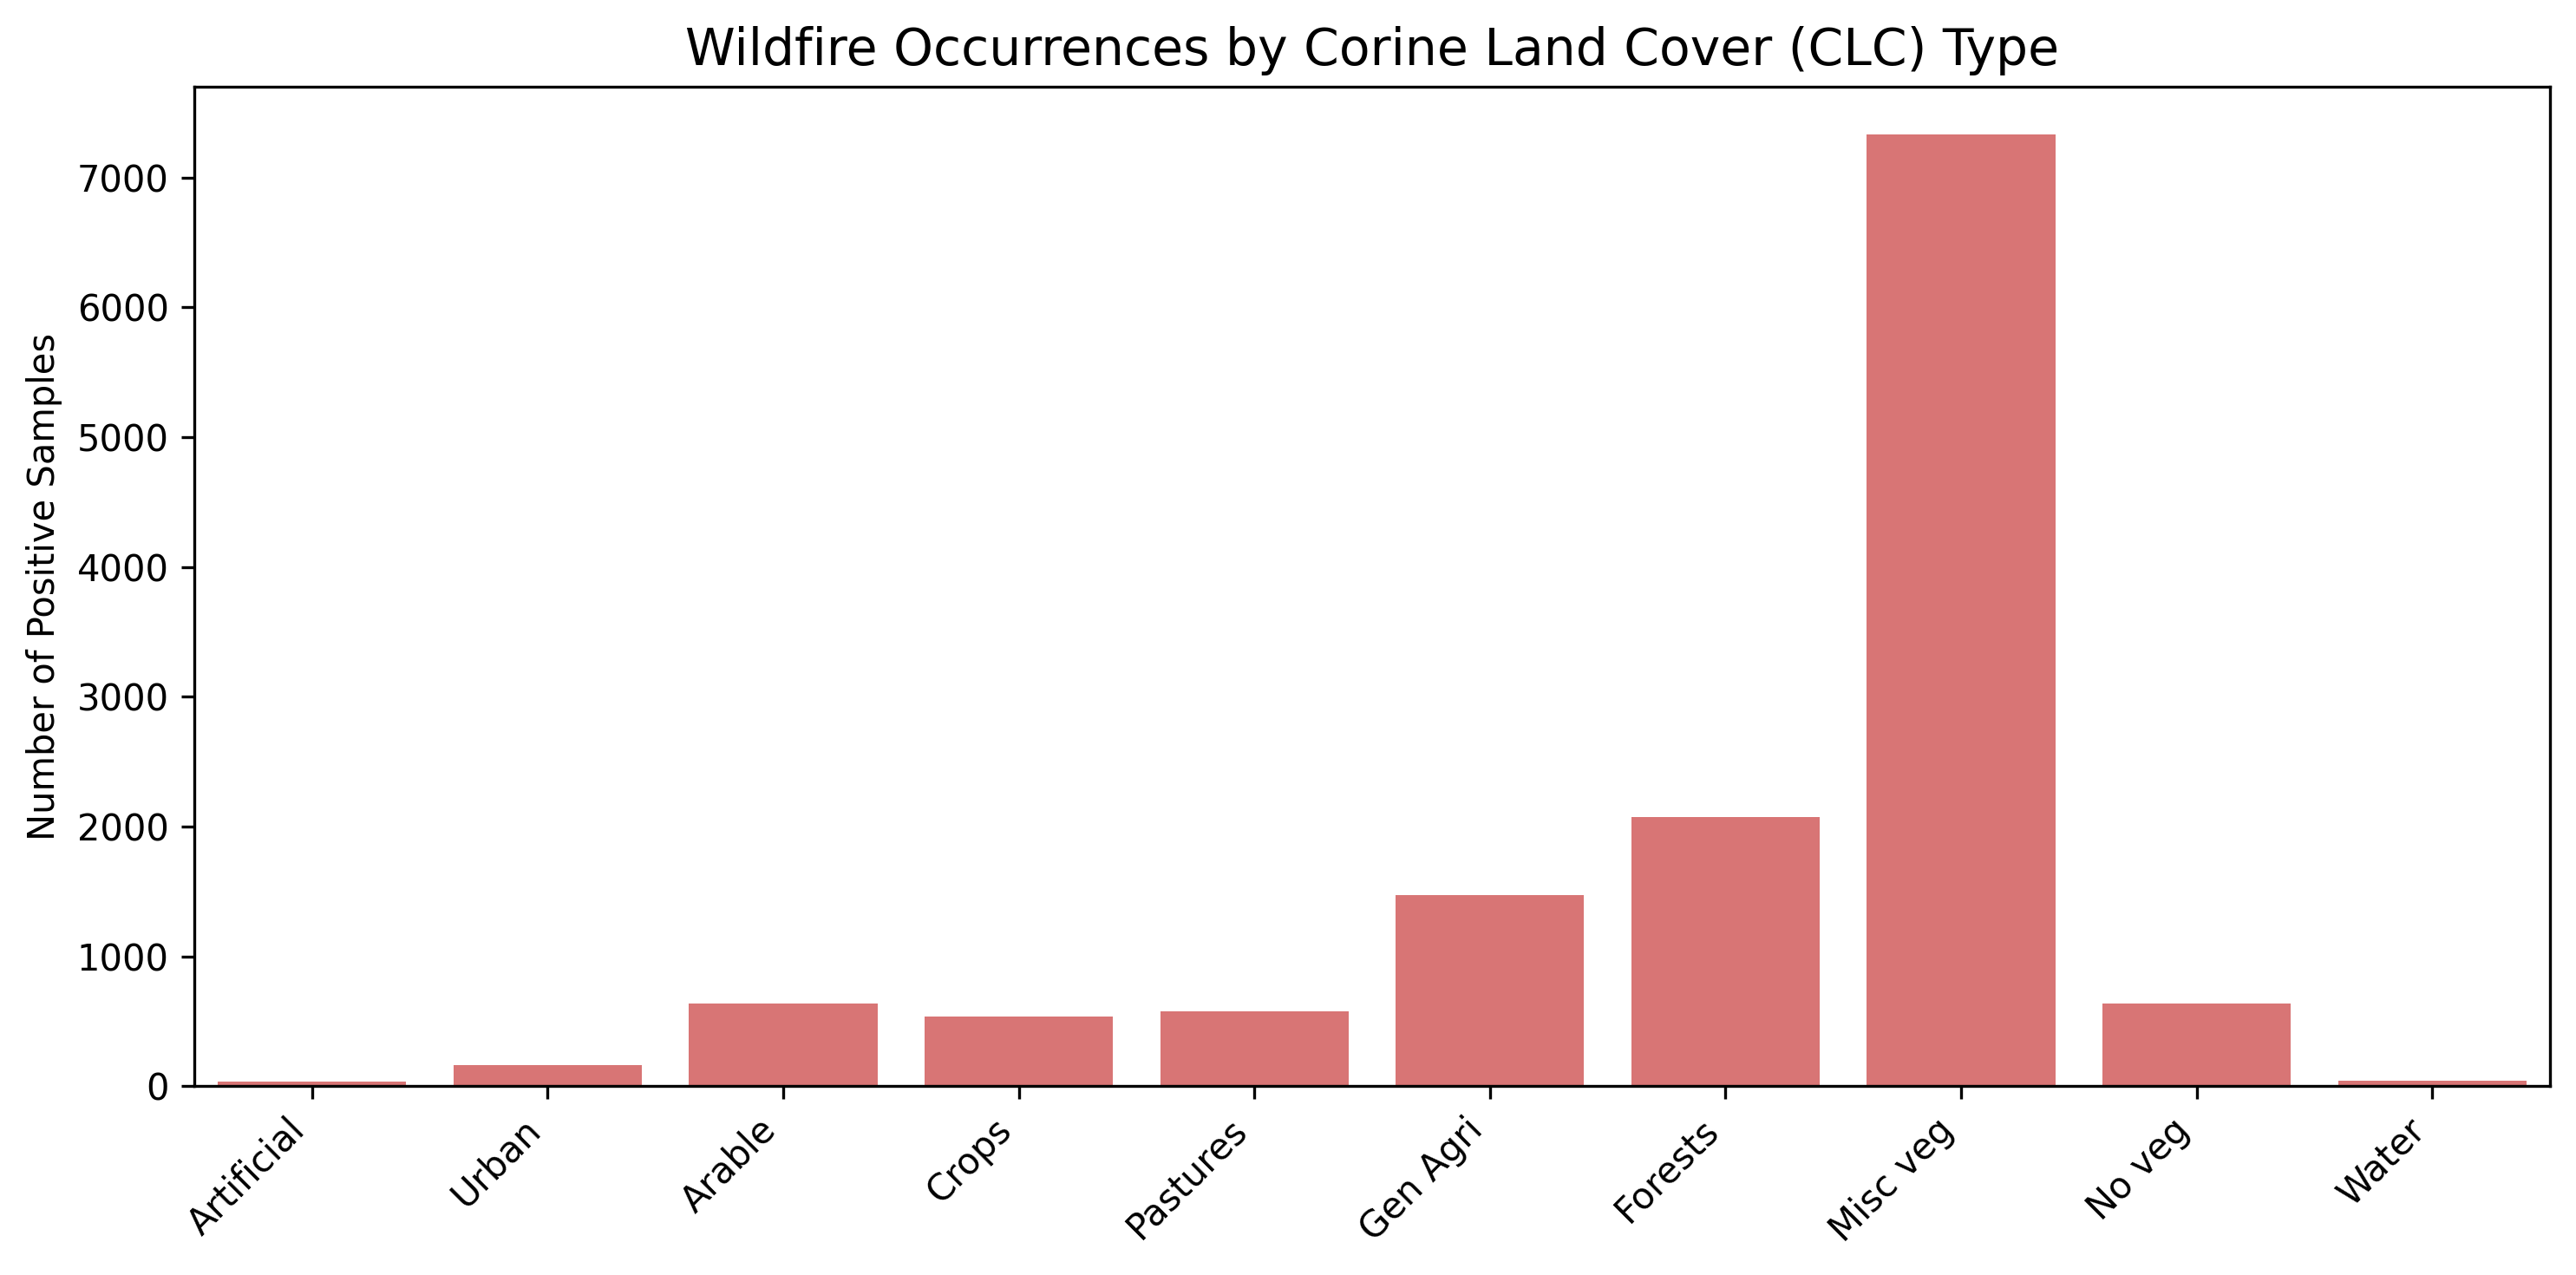
\includegraphics[width=0.9\textwidth]{img/chap2/2-3-clc.png}
    \caption{FireCube数据集中野火事件在不同土地覆盖类型(CLC)上的空间分布}
    \label{fig:2-3-clc}
\end{figure}

这一分布特征为本研究的模型架构设计提供了物理支撑。分布证明了地表覆盖类型，本质上是燃料基底的差异，对野火的发生具有较大的约束作用。这就要求模型必须具备独立剥离并感知这种地理底色的机制，而这恰恰是我们在架构中单独采用静态编码器分支，进行地貌特征提取的核心动机。

图\ref{fig:2-3-elevation-slope}展示了研究区域内野火发生频次在海拔（Elevation）与坡度（Slope）两个静态地理维度上的二维核密度分布。

\begin{figure}[htbp]
    \centering
    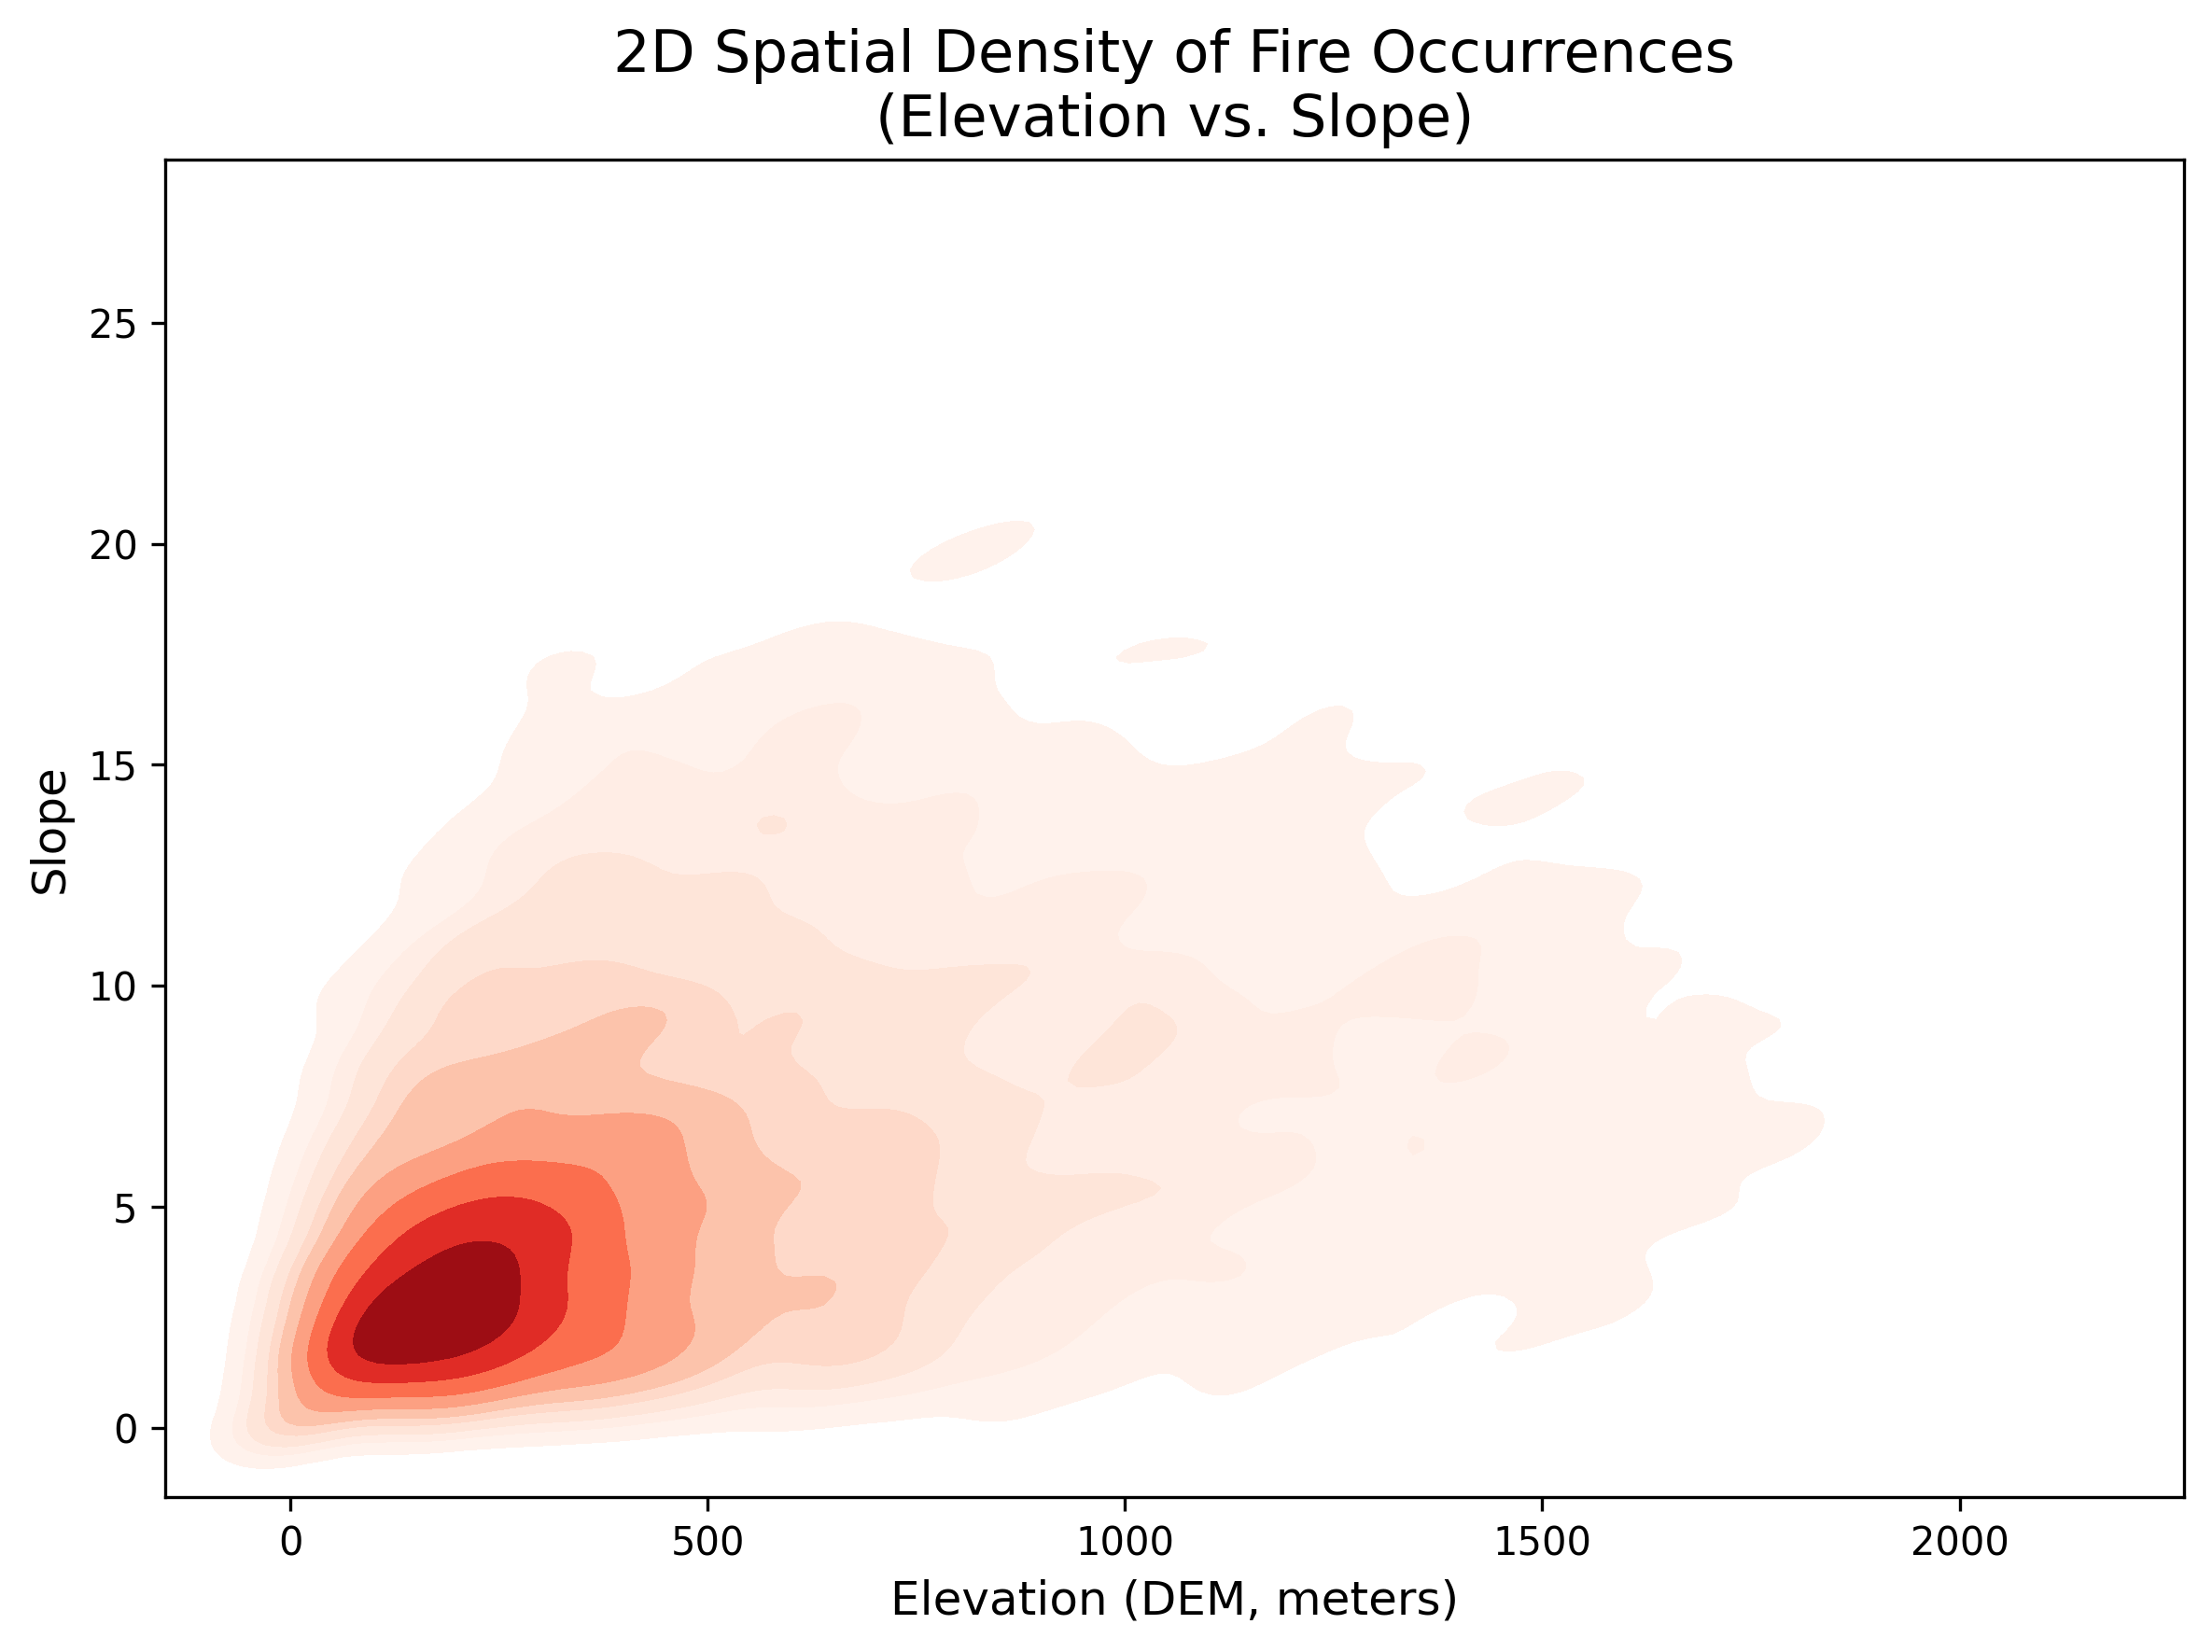
\includegraphics[width=0.8\textwidth]{img/chap2/2-3-elevation-slope.png}
    \caption{FireCube数据集中野火海拔与坡度上的二维核密度分布}
    \label{fig:2-3-elevation-slope}
\end{figure}
从图中的密度分布可以清晰地观察到，野火主要发生在海拔较低（约 0-400 米）且坡度平缓（约 0-5 度）的区域。随着海拔的升高或坡度的增加，颜色迅速变浅，说明一旦海拔升高或在陡坡地区，火灾发生频次就会断崖式下降。造成这一地理分布特征可能是因为，低海拔地区在火灾季通常有更高的气温和更强的蒸发作用，形成了易燃的环境，并且低海拔与平缓坡地往往是人类定居点、农业用地和路网密集的区域，人类活动增加了火源出现的概率。

\subsection{动态变量分析}
\label{sec:dynamic-variable-analysis}
图\ref{fig:2-3-correlation-matrix}展示了FireCube数据集正样本中的10类动态特征变量的皮尔逊相关性矩阵热力图。通过对相关性系数的分析，可以揭示气象因子在火灾发生时可能的物理机制。

首先，热力图展现了火险天气的典型特征。其中，最高气温（$Max\_t2m$）与最低相对湿度（$Min\_rh$）呈现出全图最强的负相关性（$r=−0.50$）。这符合火灾发生前的物理规律：气温的异常升高往往伴随着空气水分的剧烈蒸发，导致相对湿度骤降，从而极大地加速了地表可燃物的干燥过程。此外，最大地表气压（$Max\_sp$）与最大风速（$Max\_wind$）呈现出显著的正相关（$r=0.57$），表明气压梯度的变化是驱动大风、进而助长火势蔓延的重要动力学因素。其次，土壤湿度（$sminx$）表现出了较强的特征独立性，这表明土壤湿度是一个刻画长期干旱累积效应的变量，其变化较慢，它提供了区别于快速气象变化的独特物理信息。最后，从深度学习特征工程的角度来看，该图证明了选取的特征集合的优质性。矩阵中所有非对角线元素的绝对值均未超过0.6，表明这些动态特征之间不存在严重的多重共线性（Multicollinearity）。这说明本文选取的 10 个动态特征各自包含了相对独立的信息，特征冗余度低。这一发现确保了后续输入Swin Transformer网络的数据质量，有助于模型更稳定、高效地提取时空演变特征。

\begin{figure}[htbp]
    \centering
    \begin{minipage}{0.48\textwidth}
        \centering
        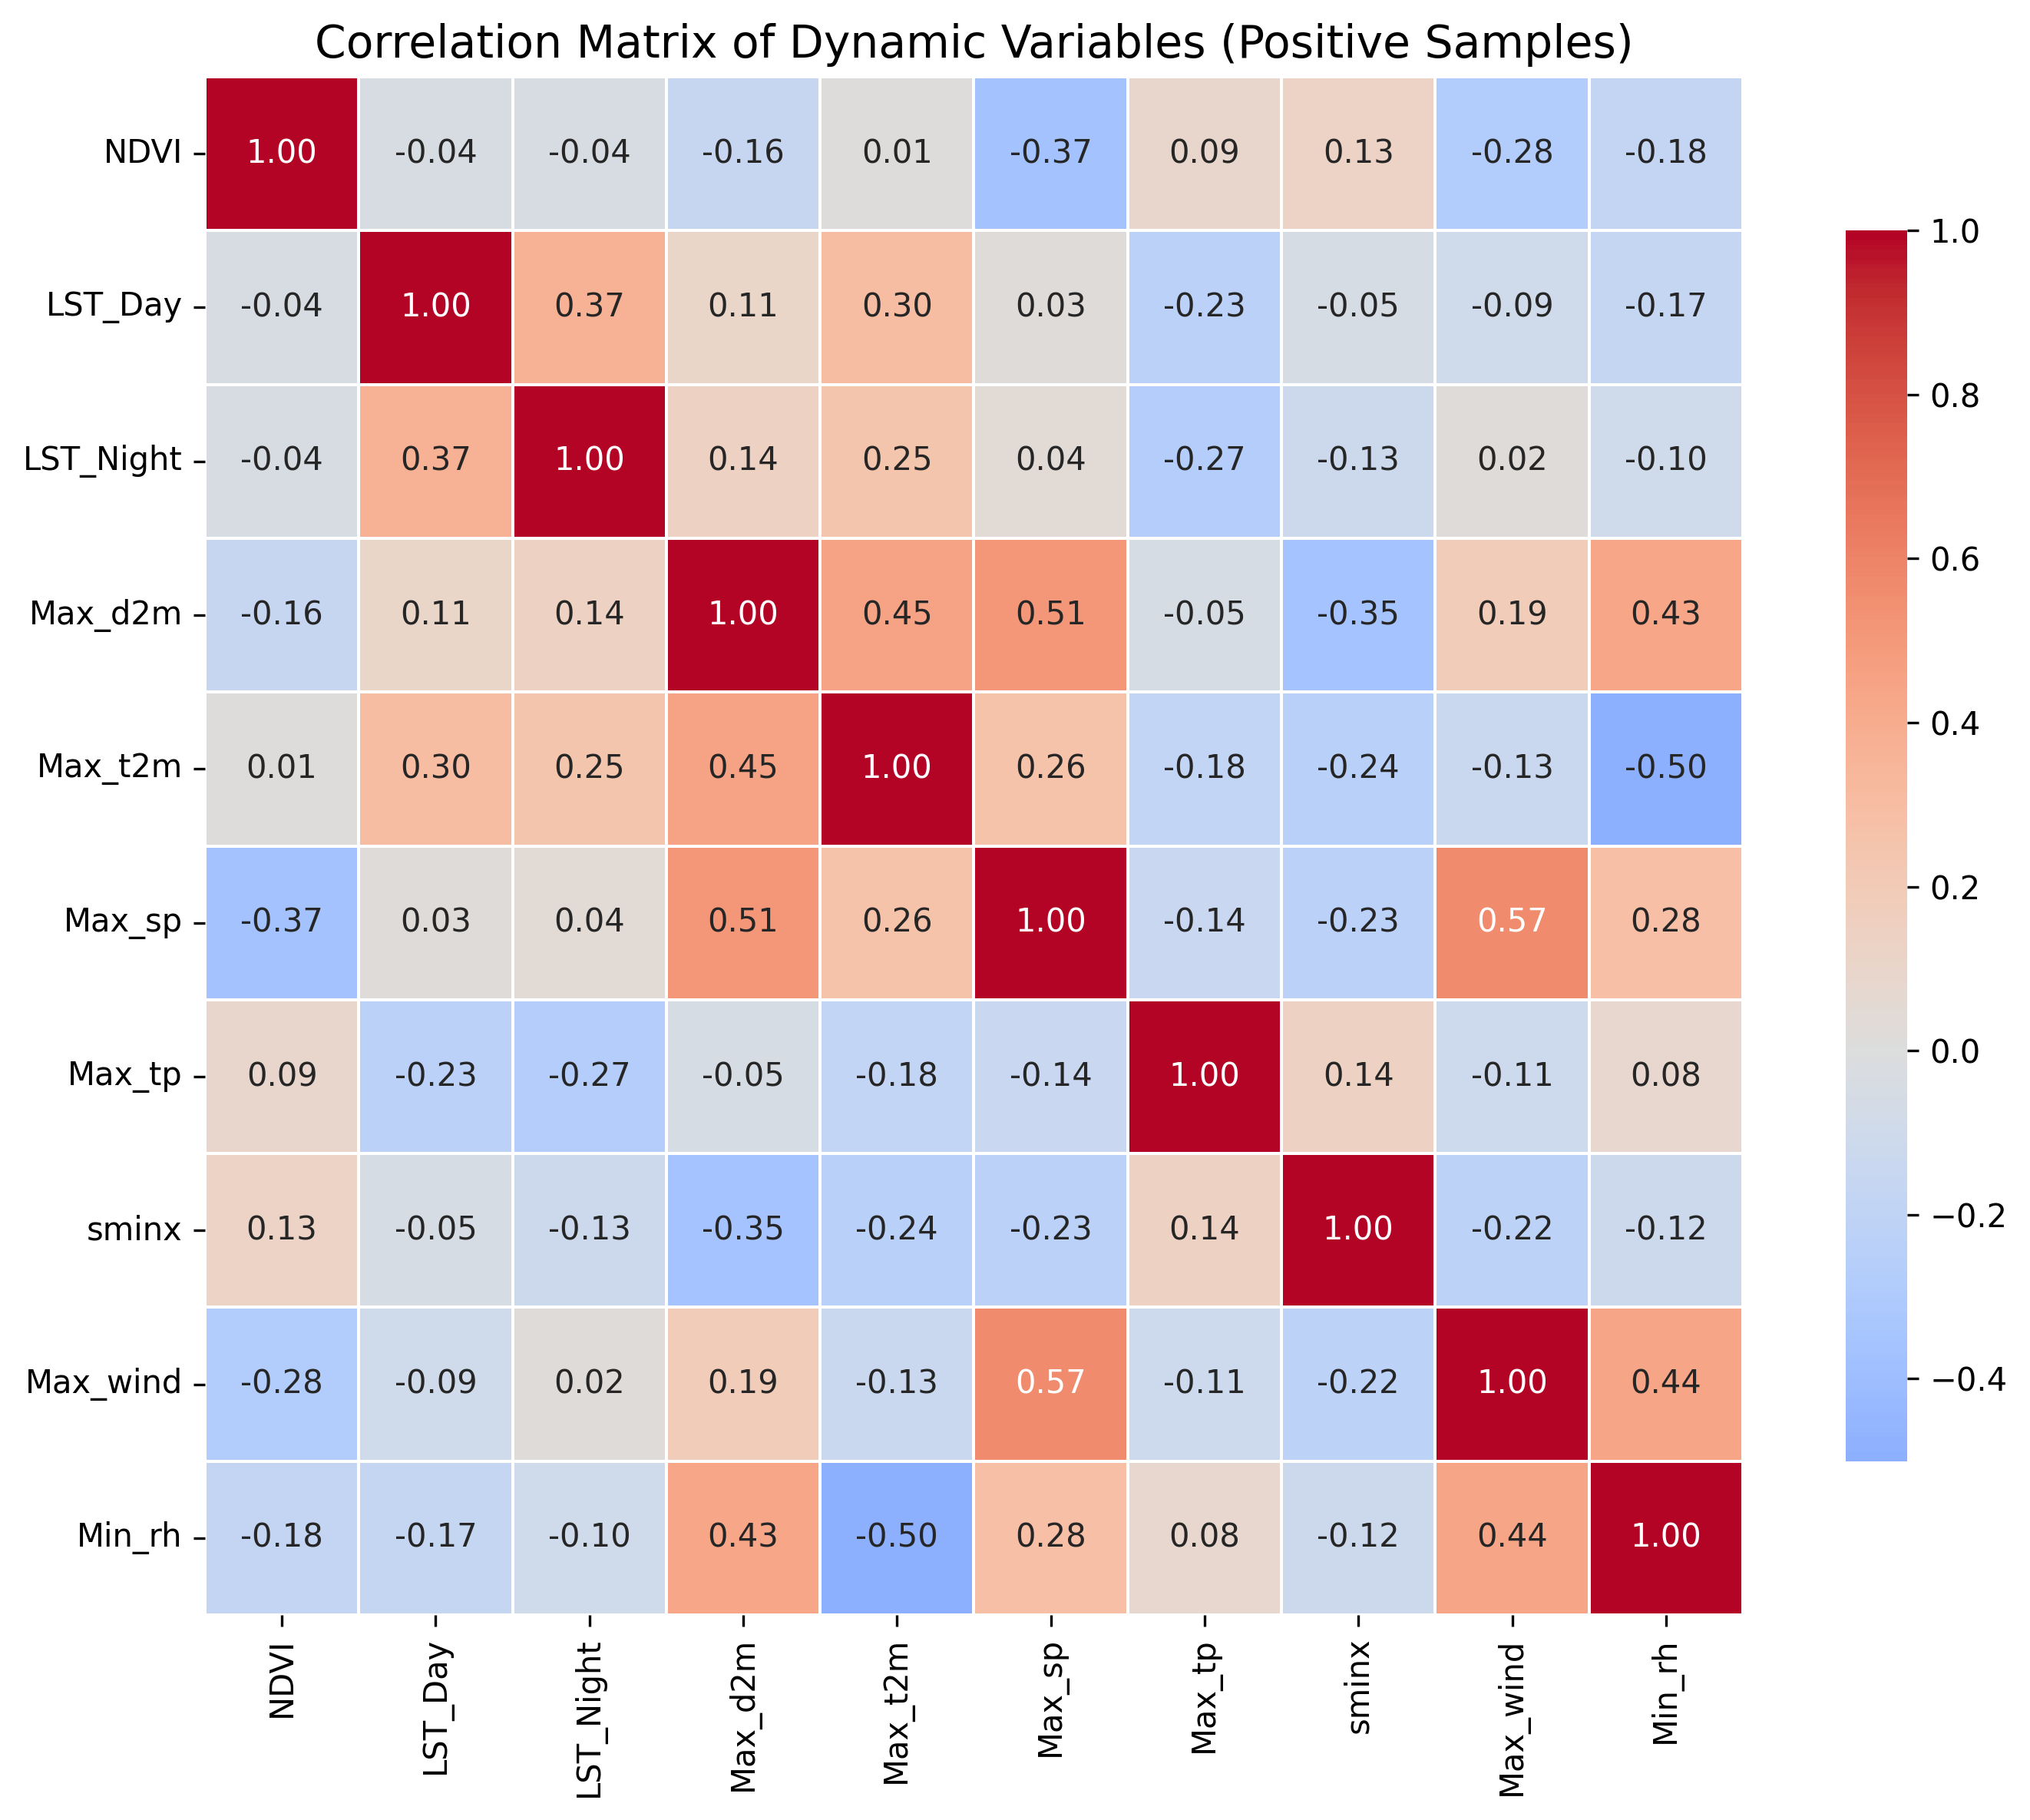
\includegraphics[width=\textwidth]{img/chap2/2-3-correlation-matrix.png}
        \caption{FireCube数据集中动态变量的皮尔逊相关性矩阵}
        \label{fig:2-3-correlation-matrix}
    \end{minipage}
    \hfill 
    \begin{minipage}{0.48\textwidth}
        \centering
        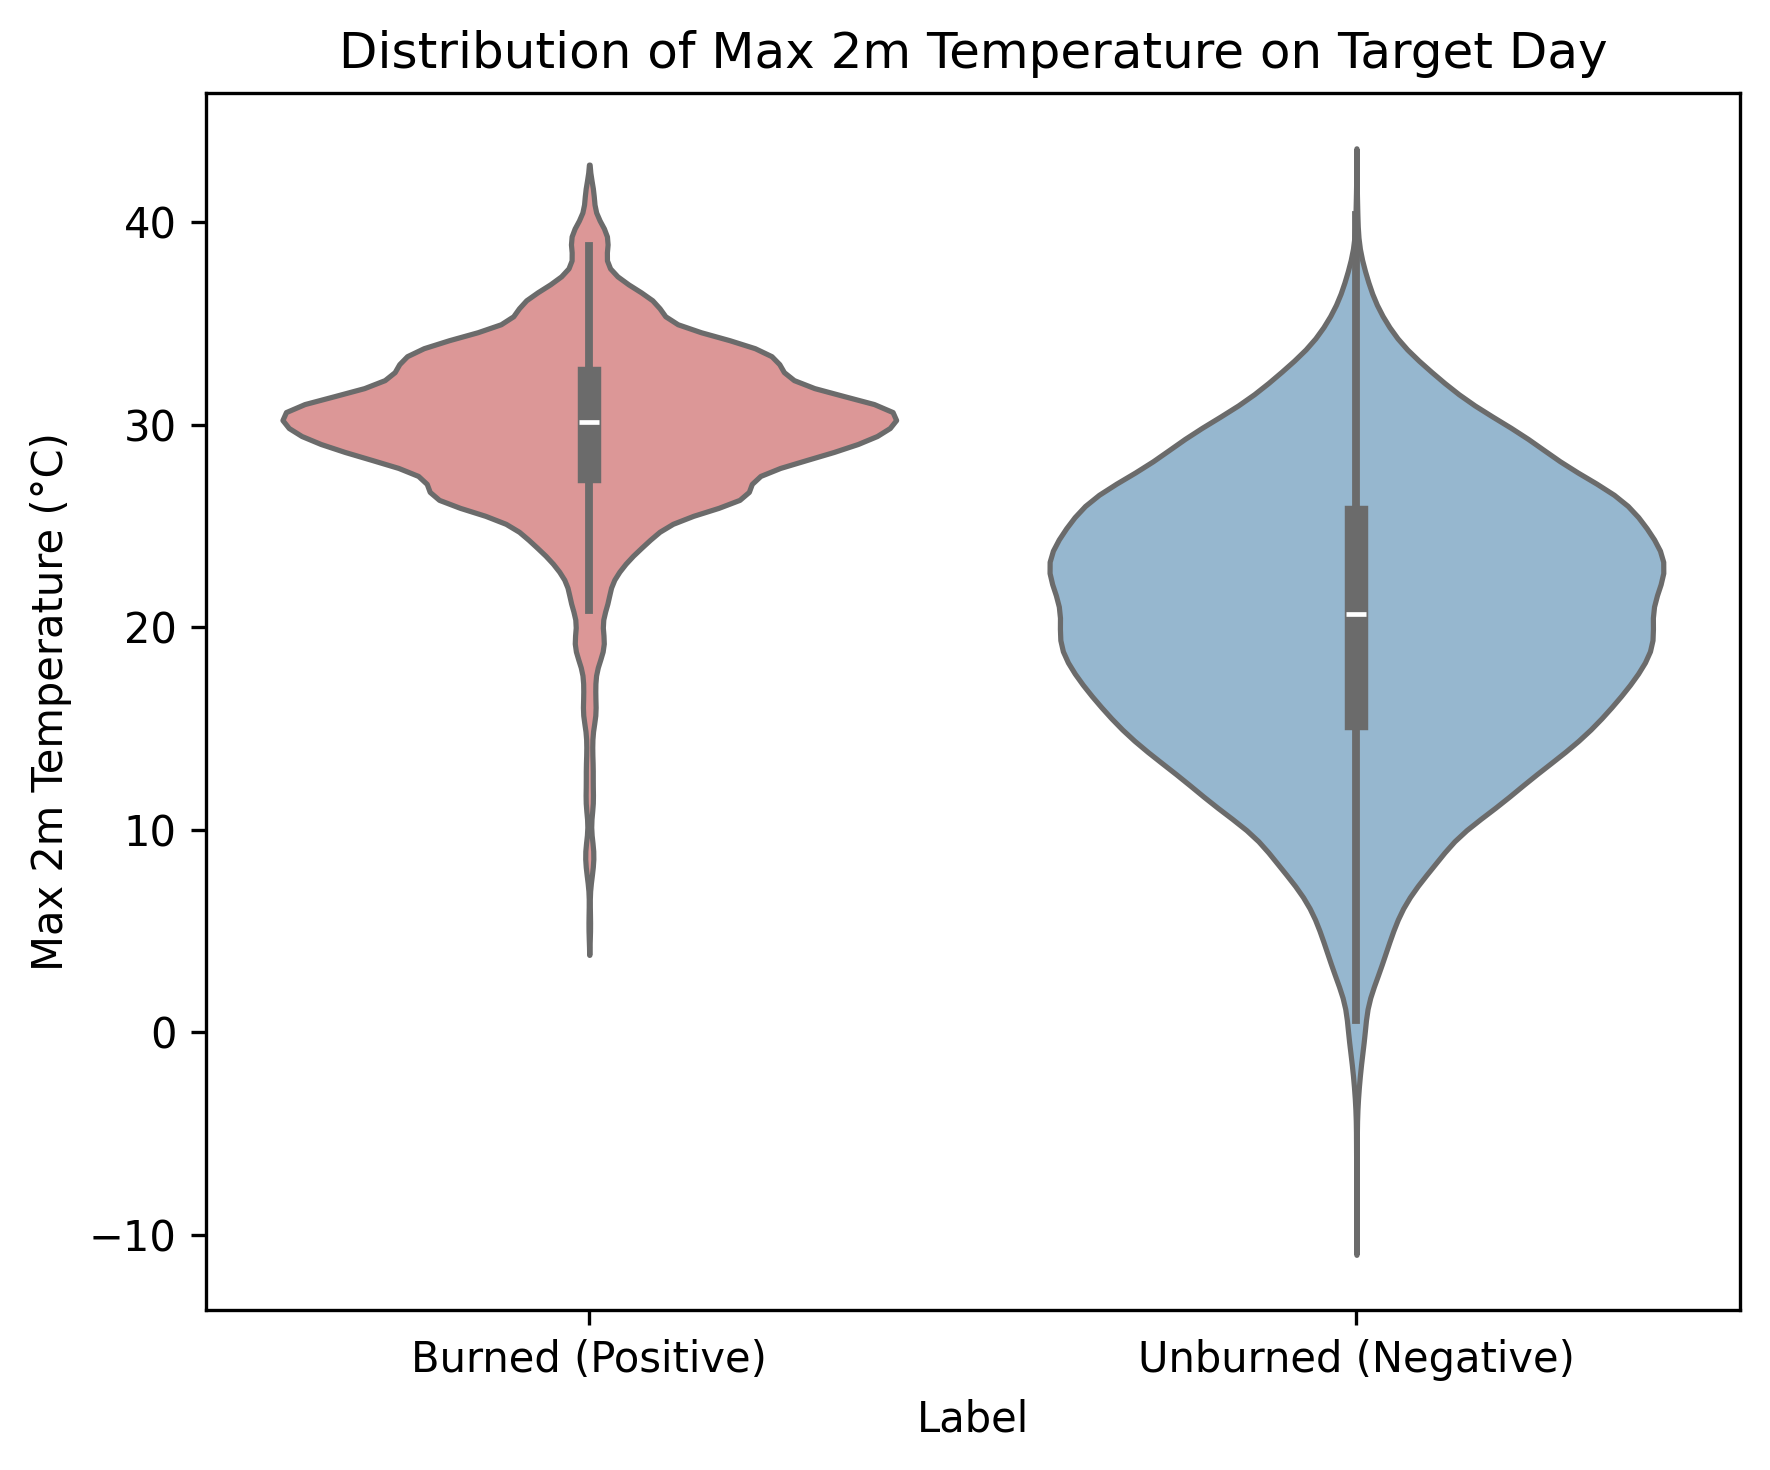
\includegraphics[width=\textwidth]{img/chap2/2-3-2m-temperature-distribution.png}
        \caption{FireCube数据集中正负样本在最高气温上的分布}
        \label{fig:2-3-2m-temperature-distribution}
    \end{minipage}
\end{figure}

图\ref{fig:2-3-2m-temperature-distribution}展示了目标日正负样本在两米处最高气温（$Max\_2m\_Temperature$）上的分布差异小提琴图。

从统计分布的形态与位置来看，起火日与非起火日的气温呈现出显著差异。未起火的负样本温度分布较为宽泛，中位数约为 21°C，反映了该地区常规气候背景下的正常自然波动。而发生野火的正样本分布较为集中，其中位数高达 30°C。这一分布特征直观地揭示了高温与野火发生的关系。同时，正负样本在$Max\_t2m$特征上的重叠度较低，表明该气象变量具有较强的判别力，验证了将其作为动态输入特征的科学性。

图\ref{fig:10-day-evolution}展示了目标日前 10 天示例气象与地表特征的时序演变图。图中实线代表所有正样本或负样本的平均值，阴影区域表示 95\% 置信区间。其中图\ref{fig:2-3-soil-moisture}展示了土壤湿度的演变轨迹，图\ref{fig:2-3-temperatures-10-days}展示了最高气温的演变轨迹。
\begin{figure}[H]
    \centering
    % 第一张子图 (a)
    \begin{subfigure}[b]{0.48\textwidth}
        \centering
        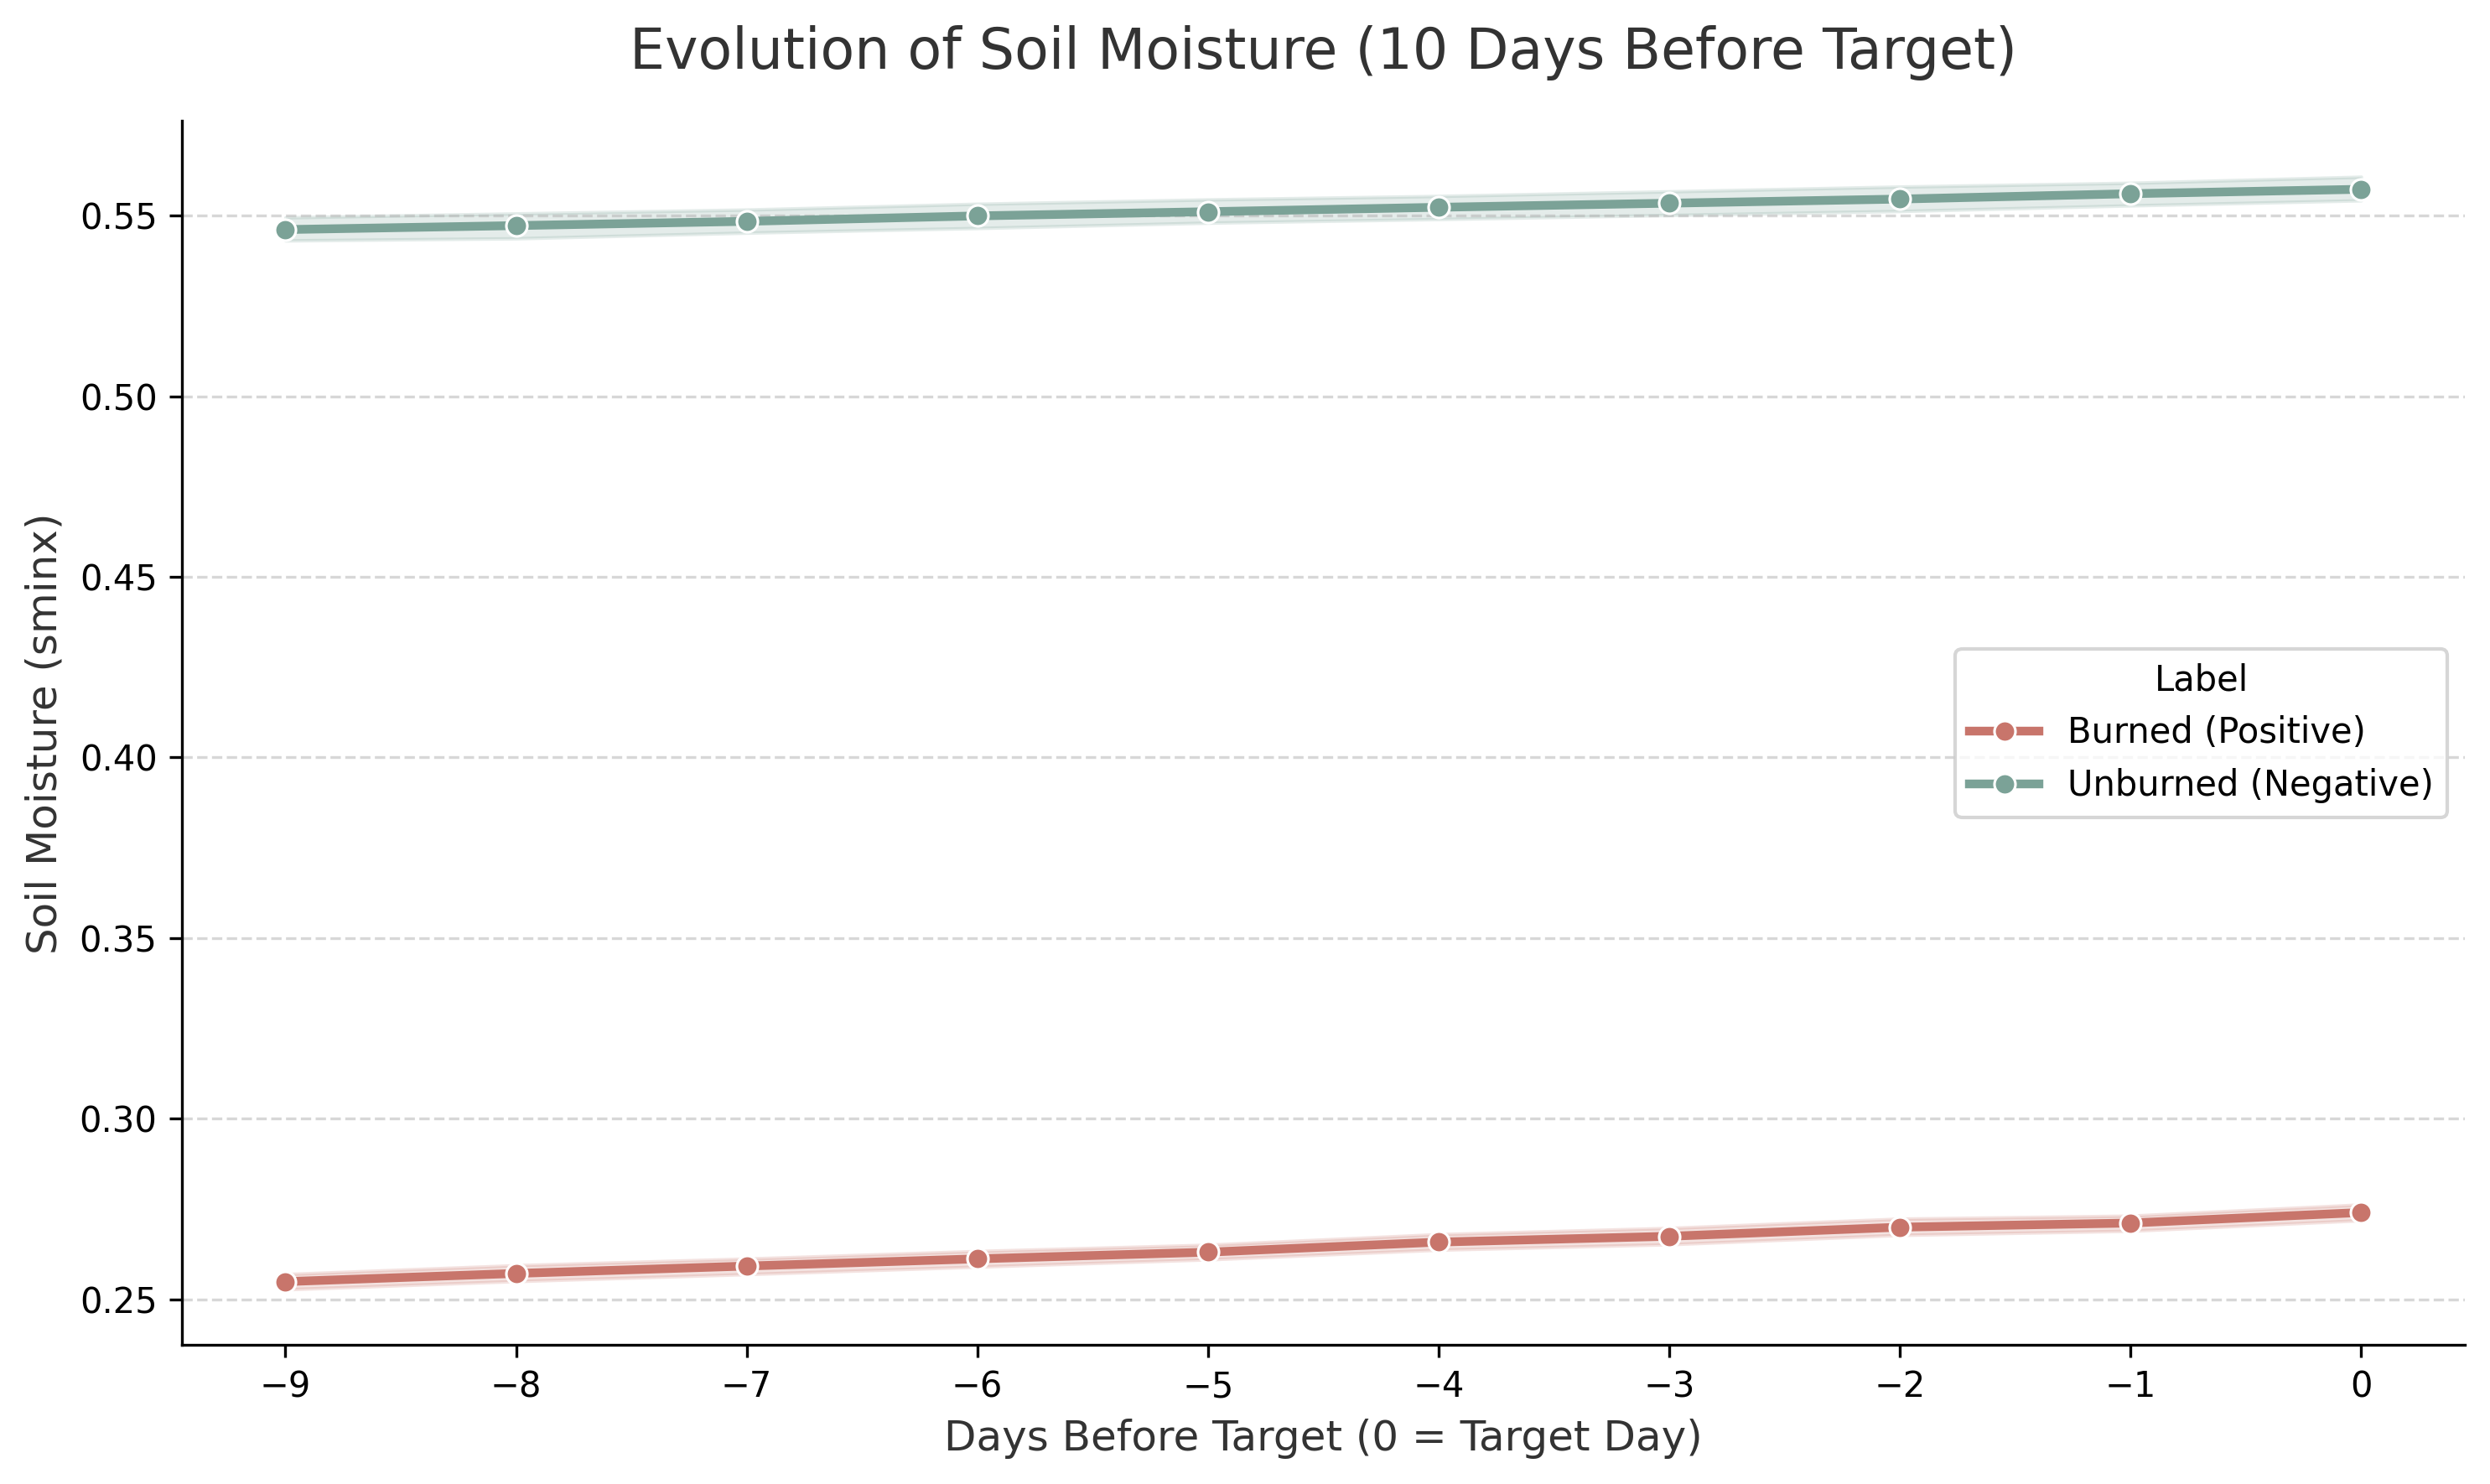
\includegraphics[width=\textwidth]{img/chap2/2-3-soil-moisture.png}
        \caption{土壤湿度的演变轨迹} % 这里写(a)图的标题，(a)会自动生成
        \label{fig:2-3-soil-moisture}
    \end{subfigure}
    \hfill 
    % 第二张子图 (b)
    \begin{subfigure}[b]{0.48\textwidth}
        \centering
        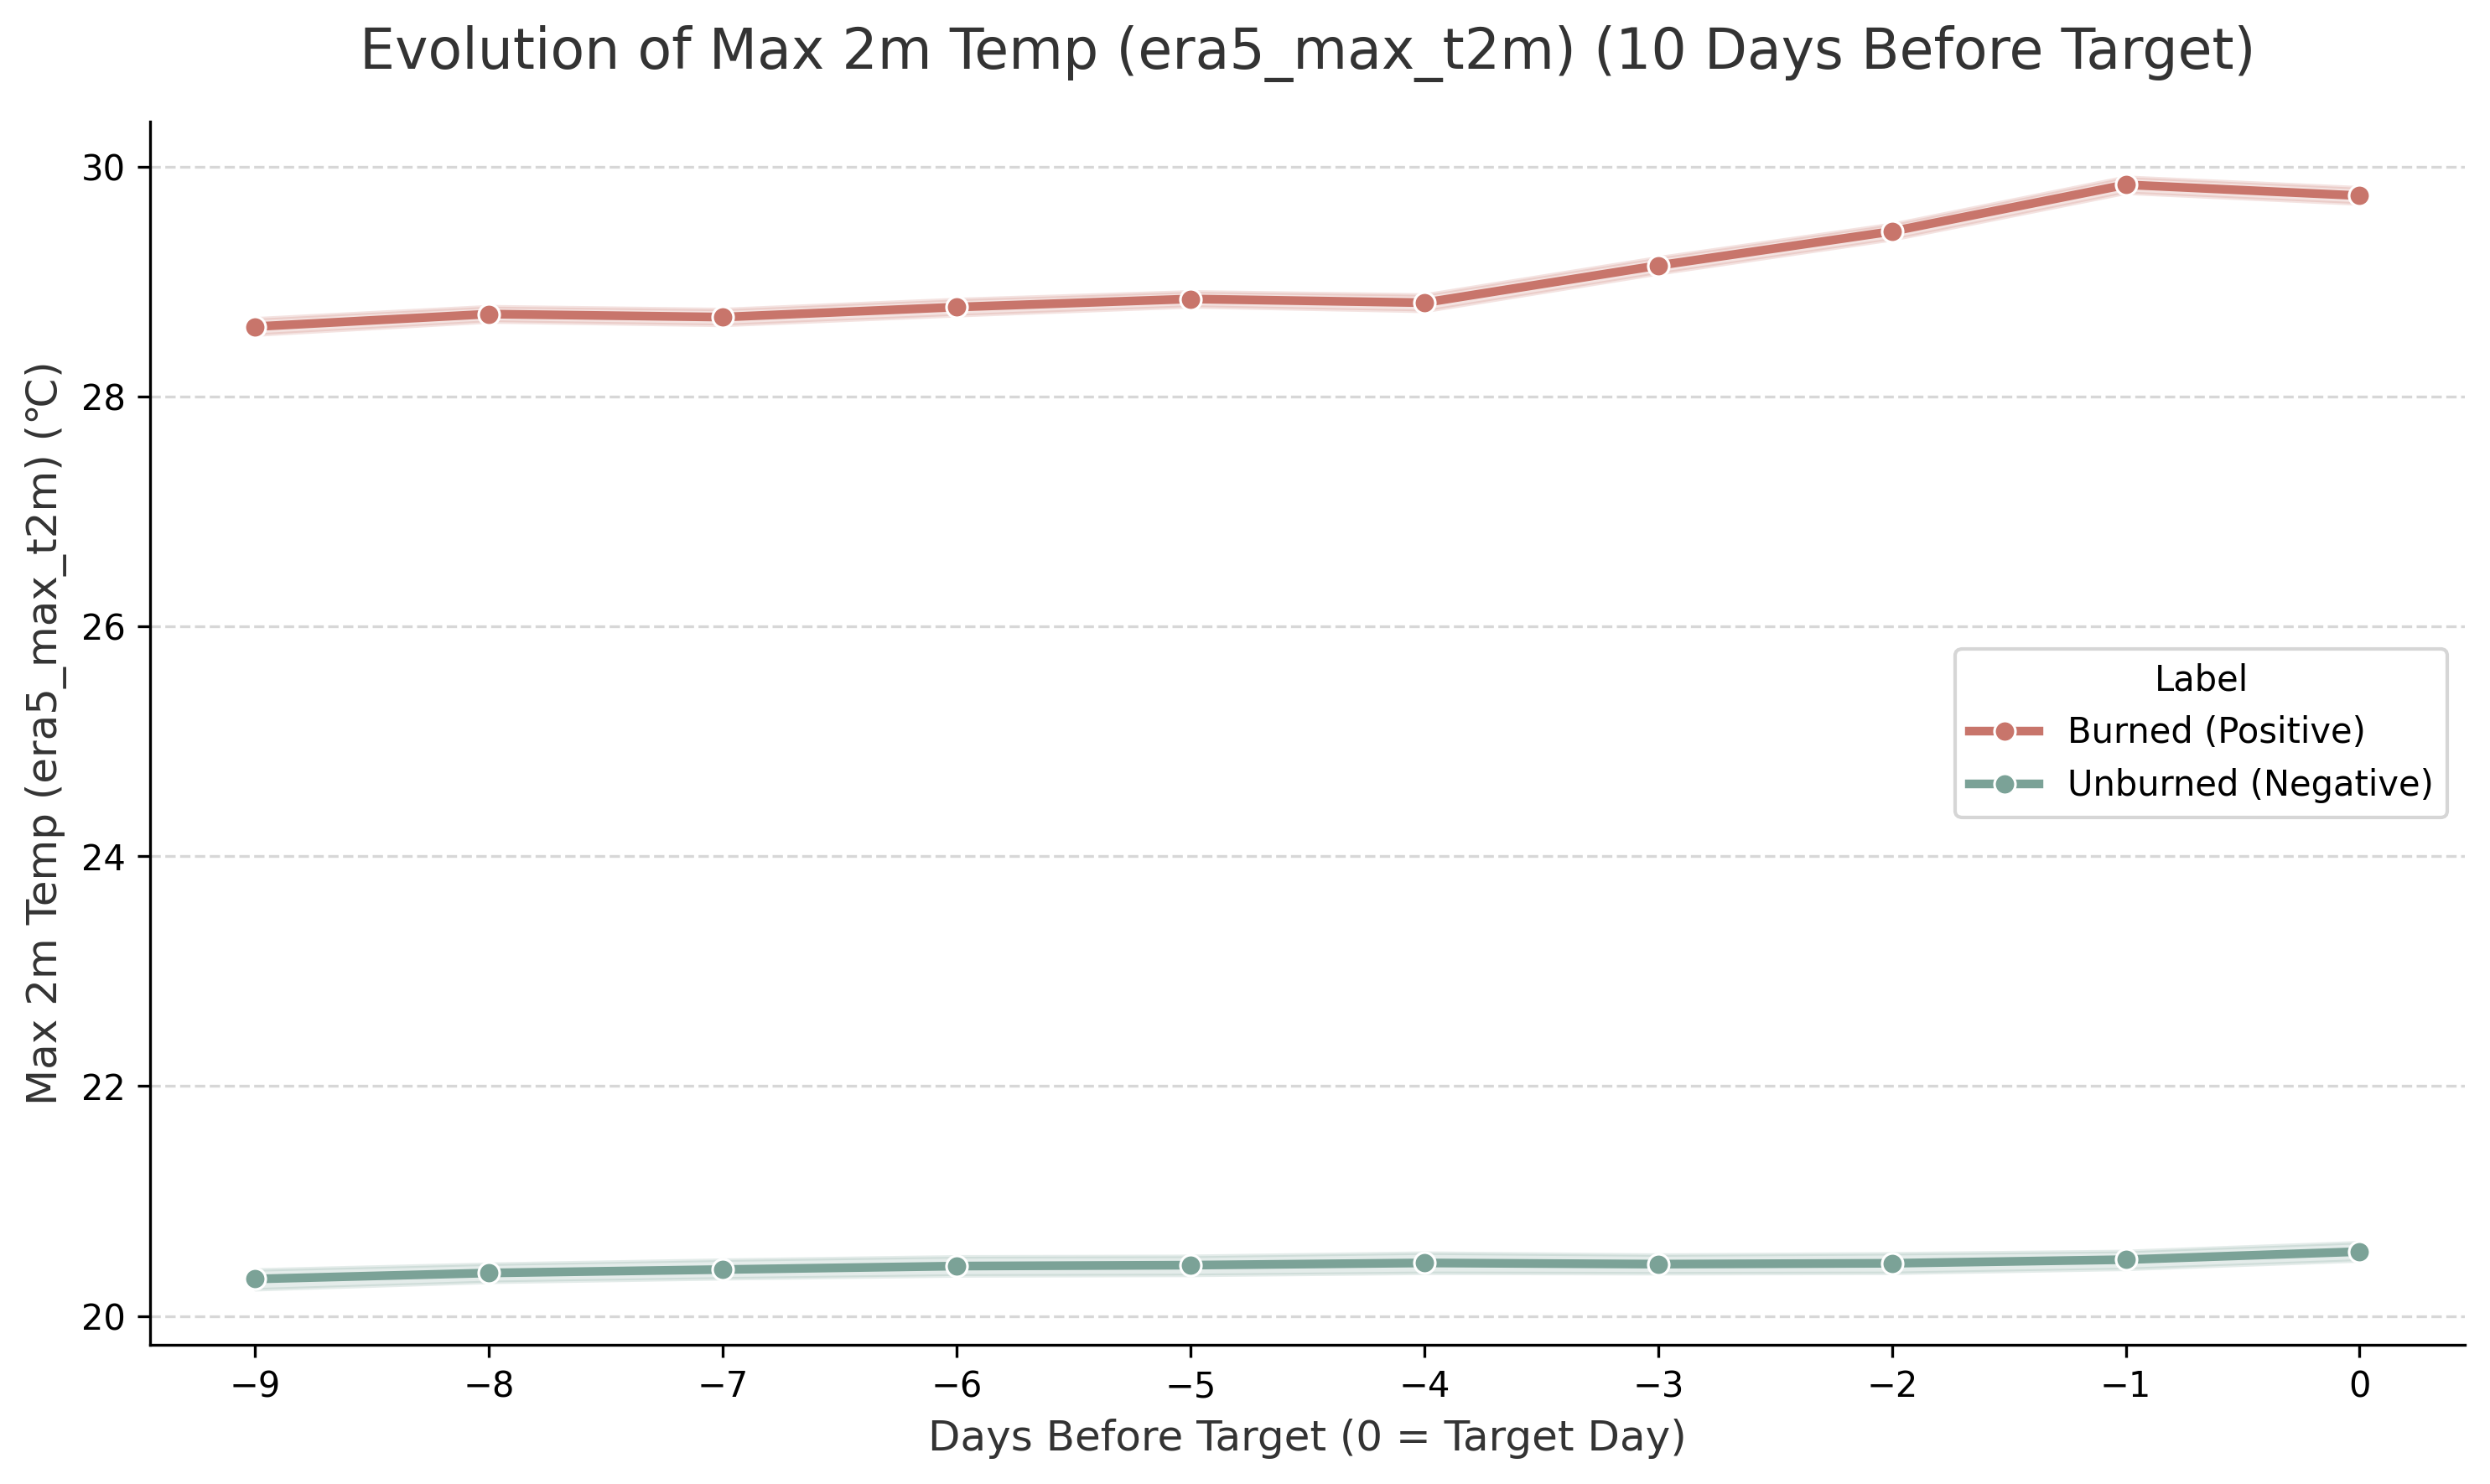
\includegraphics[width=\textwidth]{img/chap2/2-3-temperatures-10-days.png}
        \caption{最高气温的演变轨迹} % 这里写(b)图的标题，(b)会自动生成
        \label{fig:2-3-temperatures-10-days}
    \end{subfigure}
    % 整个大图的主标题
    \caption{目标日前 10 天关键气象与地表特征的时序演变图。图中实线代表正负样本的平均值，阴影区域表示 95\% 置信区间。}
    \label{fig:10-day-evolution} % 这是整个大图的引用标签
\end{figure}

在土壤湿度演变轨迹中，在绝对数值基线上，正负样本呈现出显著的差异，负样本土壤湿度大，基本在0.55左右，而正样本的土壤湿度低于0.3；在演变趋势上，负样本的土壤湿度变化范围非常小，而正样本的土壤湿度缓慢上升，变化范围相对大一些，符合野火发生的客观物理规律。在最高气温的演变轨迹中这一现象更加明显，正样本的基础最高温度比负样本高出约9°C，且负样本的温度在10天的时间尺度中几乎保持不变，而正样本呈现出温度升高的趋势。同时，土壤湿度和最高气温这两组变量之间也形成了一定的对比，在演变趋势上，表现出典型的“快慢变量耦合”特征。土壤湿度作为慢变量，在 10 天内保持相对平缓的低位震荡，表明地表已处于极度干燥的临界状态。而最高气温作为快变量，其正样本曲线在起火前的10天内呈现出一条明显的持续攀升轨迹。

上述多组特征变量分析得出的该数据集分布规律，为本研究的模型架构设计提供了直接的理论指导。具体而言，野火的发生并非由单一因素主导，本质上是静态地理约束与动态气象演变高度耦合的复杂物理过程。地表形态与植被覆盖这层静态底色，决定了灾害波及的地理空间上限，赋予了该区域特定的空间易感性；而究竟在哪个节点真正起火，则更多地取决于动态气象因子的变化。

因此，静态变量与动态变量缺一不可。这一结论直接促使本研究设计了双分支网络架构，能够同时处理不同特征，通过静态 2D 分支编码地理空间先验，利用 3D 时序分支捕获气象序列的动态演变趋势，最终在特征融合阶段实现深度融合，从而提升模型的野火预测能力。
    \chapter{基于物理信息启发的双分支Swin Transformer预测模型的架构设计}
\label{chap:3}

\section{总体架构设计思路}
\label{sec:3-1}
野火蔓延是一个高度复杂的非线性动力学过程，受到气象、地形与植被等多种环境因素的共同影响，并表现出明显的多尺度时空耦合特性。现有深度学习方法大多采用“全变量直接拼接”的方式，将静态与动态特征统一输入模型进行学习。虽然这种方法实现简单，但往往忽略了不同类型变量在时间和物理意义上的差异，尤其难以有效刻画气象因子背后所蕴含的热力学过程与演化规律。

针对上述问题，本章提出一种基于物理启发的时空解耦双分支 Swin Transformer 野火预测模型。该模型从特征属性出发，将静态地理信息与动态气象信息分别建模，通过双分支结构实现时空特征的解耦学习。同时，在动态分支中引入与火灾传播相关的物理先验，以增强模型对环境变化过程的表征能力，在提升预测性能的同时提高结果的可解释性。模型整体框架如图\ref{fig:3-1-pipeline}所示。

时空特征解耦原则主要是由于大气环境因子的演化周期存在本质差异。地形地貌等属于静态空间特征，在短期的预测时间窗口内几乎不变。气象条件则属于动态时空特征，呈现出随时间演变的特征。若统一采用三维网络处理，会导致模型对静态背景进行冗余建模，增加过拟合风险。本架构采用双分支编码策略，均基于Swin Transformer构建，利用二维分支专门提取静态特征，三维分支提取动态气象特征。两条分支独立编码，并在后续利用地理感知交叉注意力机制进行融合，有效提升了模型的计算效率与预测精度。

物理机制引导原则旨在弥补模型缺乏物理先验的缺陷。在数据输入阶段，本研究将气温与露点温度重构为饱和水汽压差（Vapor Pressure Deficit，VPD）。这一预处理规避了神经网络拟合复杂热力学公式的困难，使模型能够直接感知可燃物的水分状态。在特征融合阶段，针对传统注意力机制均匀发散的局限，本架构将风场矢量作为物理偏置注入交叉注意力模块。通过计算风向与空间相对向量的点积，模型能够捕捉更多风向信息，更契合野火随风蔓延的气象动力学规律。

\begin{figure}[htbp]
    \centering
    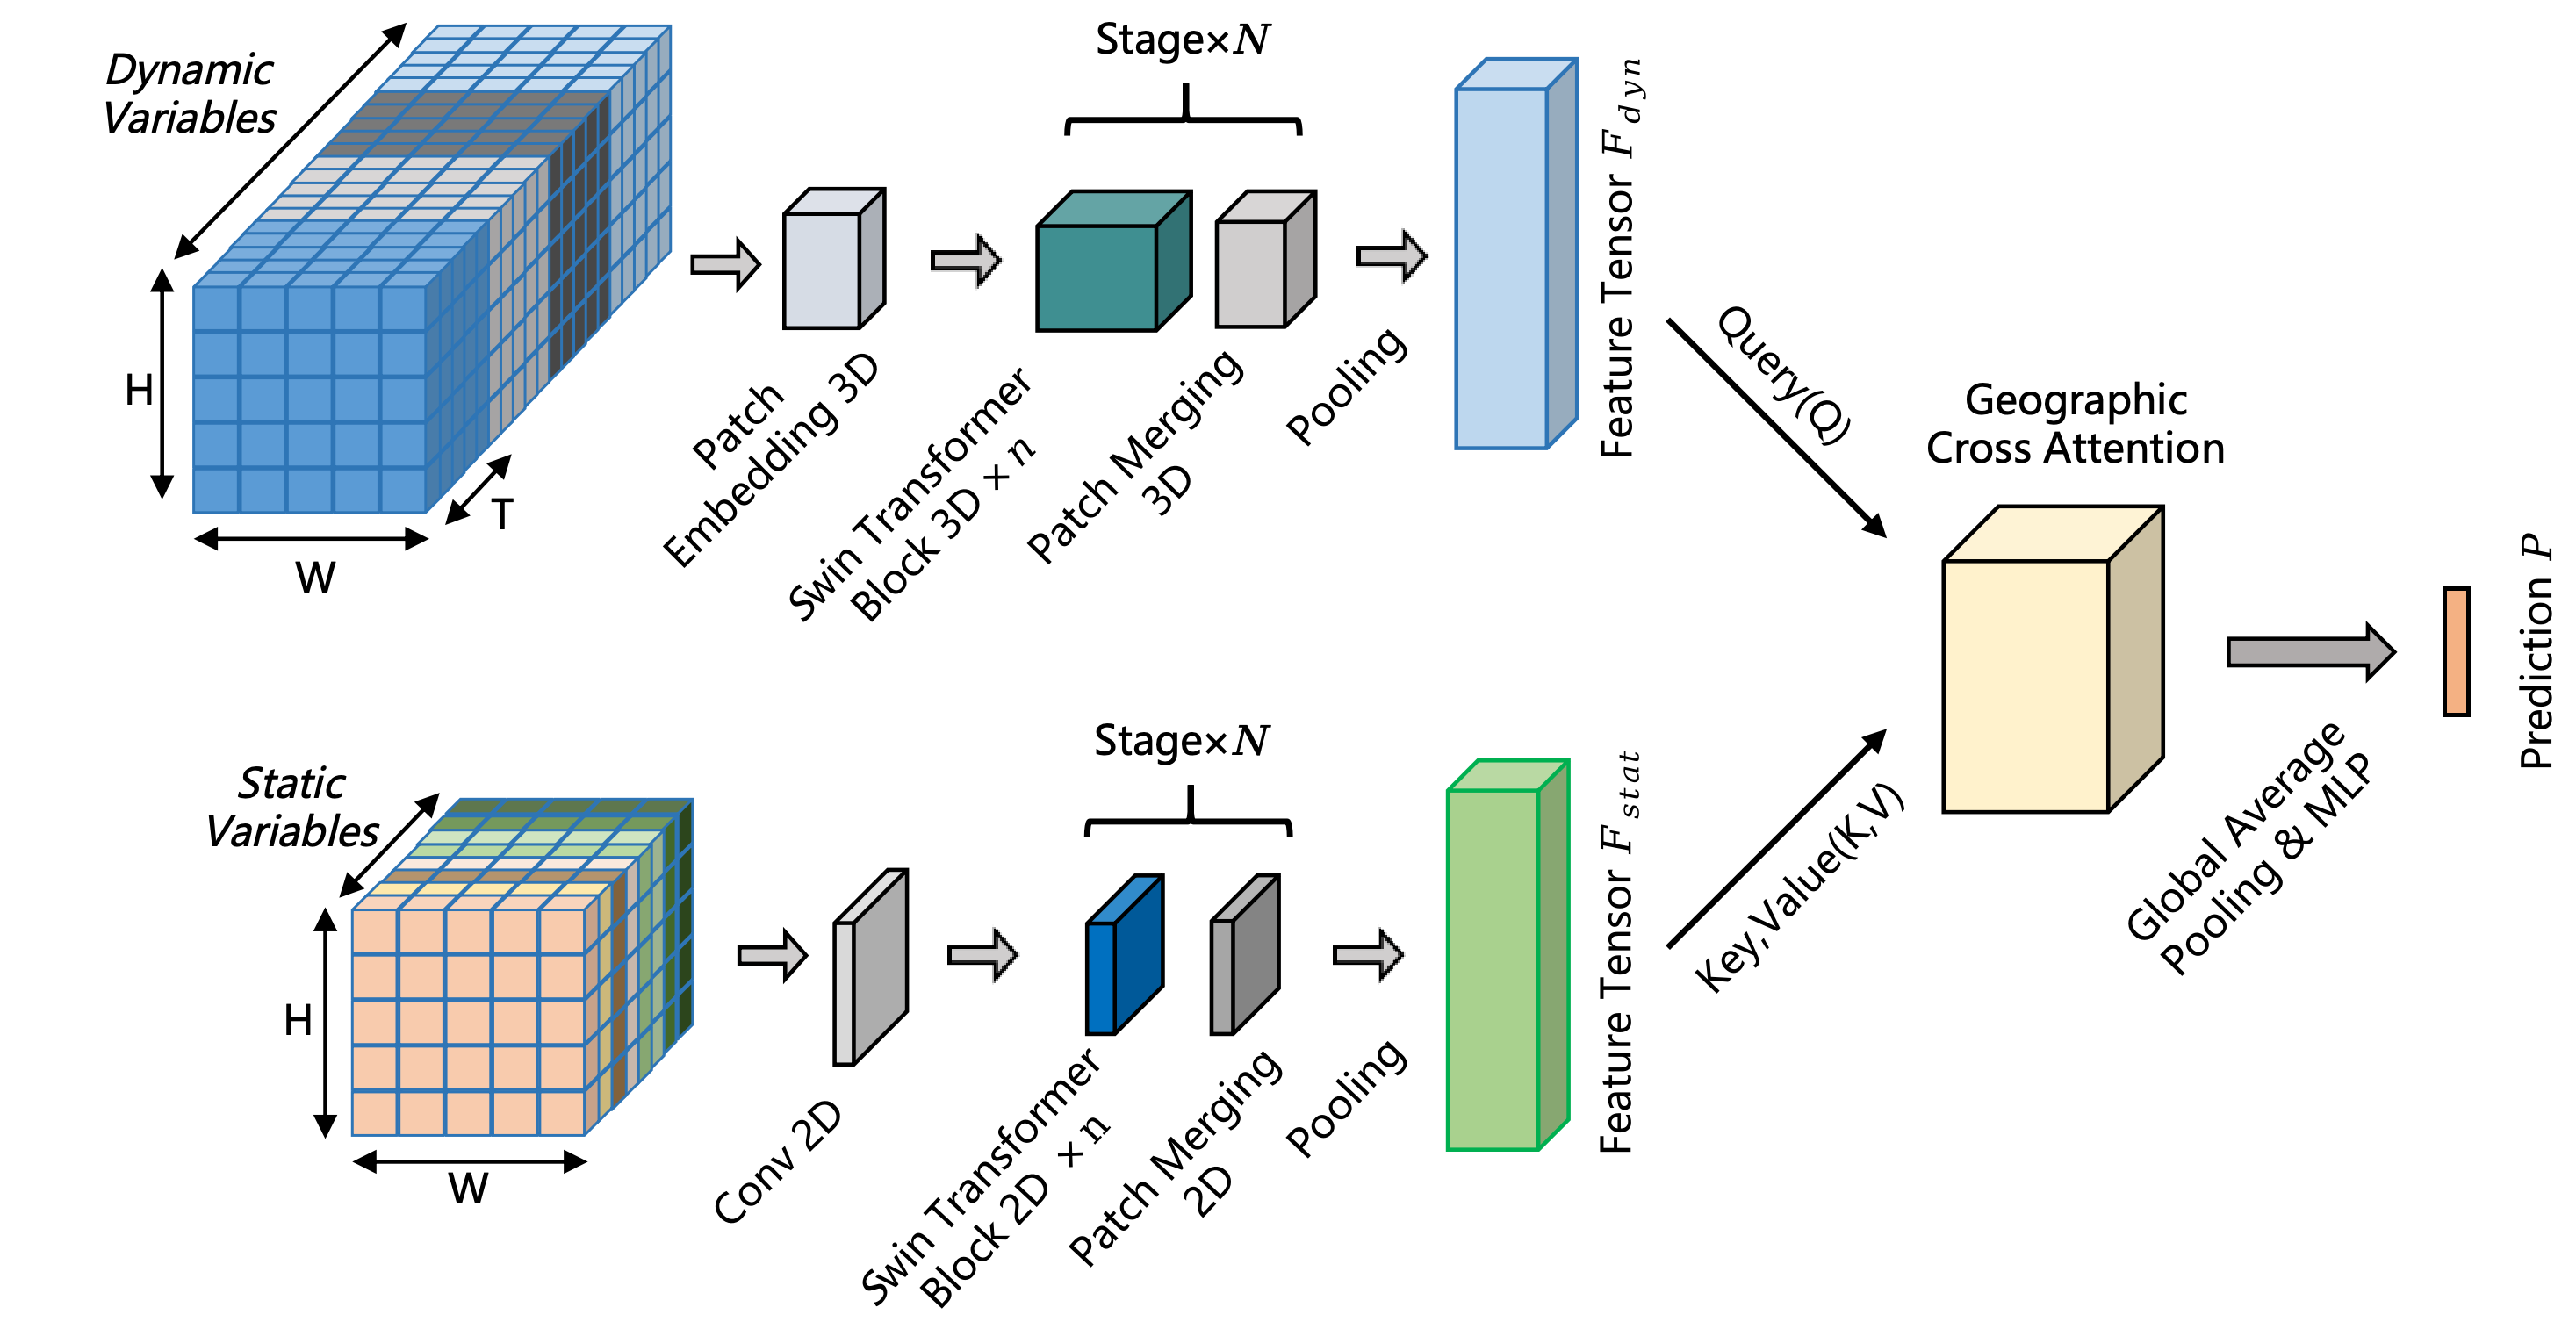
\includegraphics[width=0.9\textwidth]{img/chap3/3-1-pipeline.png}
    \caption{预测模型整体架构设计}
    \label{fig:3-1-pipeline}
\end{figure}

\section{Swin Transformer基础原理}
\label{sec:3-2}
Swin Transformer架构由微软亚洲研究院在2021年提出\cite{liu2021swin}。在计算机视觉领域，卷积神经网络（CNN）长期占据主导地位。然而，受自然语言处理（NLP）领域 Transformer\cite{vaswani2017attention} 架构巨大成功的启发，研究者开始探索如何利用其核心的自注意力机制（Self-attention）来建模数据中的长程依赖关系。Vision Transformer（ViT）是将 Transformer 直接应用于视觉任务的先驱工作\cite{dosovitskiy2020image}。它通过将图像划分为固定大小的斑块（Patches），并将每个patch视为一个token输入到Transformer 编码器，证明了在超大规模数据集预训练下，Transformer 能够达到甚至超越 CNN 的性能。然而，ViT 在作为通用骨干网络时面临两大核心挑战，一是尺度不适配，ViT 生成的是单分辨率的低分辨率特征图，难以应对视觉图像尺度变化剧烈的任务；二是计算复杂度过高，ViT 的自注意力计算是在全局范围进行的，其计算复杂度与图像尺寸成平方级增长（O${(hw)}^2$），这使得处理高分辨率图像变得异常昂贵。

为了解决上述问题，\textcite{liu2021swin}提出了 Swin Transformer，它能够作为一种新的视觉Transformer，成为计算机视觉领域的通用骨架。Swin Transformer是一个分层的Transformer，输入的特征通过滑动窗口（\textbf{S}hifted \textbf{Win}dows）来计算。滑动窗口的方案将自注意力（Self-Attention）计算局限于不重叠的局部窗口，同时允许跨窗口连接，从而提高了效率。这种分层架构具有在不同尺度建模的灵活性，并且相对于图像大小具有线性计算复杂度。

图\ref{fig:3-2-swintransformer}展示了Swin Transformer的整体架构，Swin Transformer的参数可以调整，图中所示为\cite{liu2021swin}中提及的参数量最小的版本，Swin-T（C = 96, layer numbers = {2, 2, 6, 2}）。对于一张RGB图像的输入，如图\ref{fig:3-2-swintransformer}(a)所示，Swin Transformer首先通过像ViT一样的切片（Patch Splitting）模块将输入RGB图像拆分为不重叠的Patch。每个Patch都被视为一个token，其特征被设置为原始像素RGB值的拼接。若使用的Patch大小为$4\times 4$，则每个Patch的特征维数为$4\times 4\times 3=48$。在该原始值特征上施加线性嵌入层（Embedding），将其投影到任意维度（记为C）。

\begin{figure}[htbp]
    \centering
    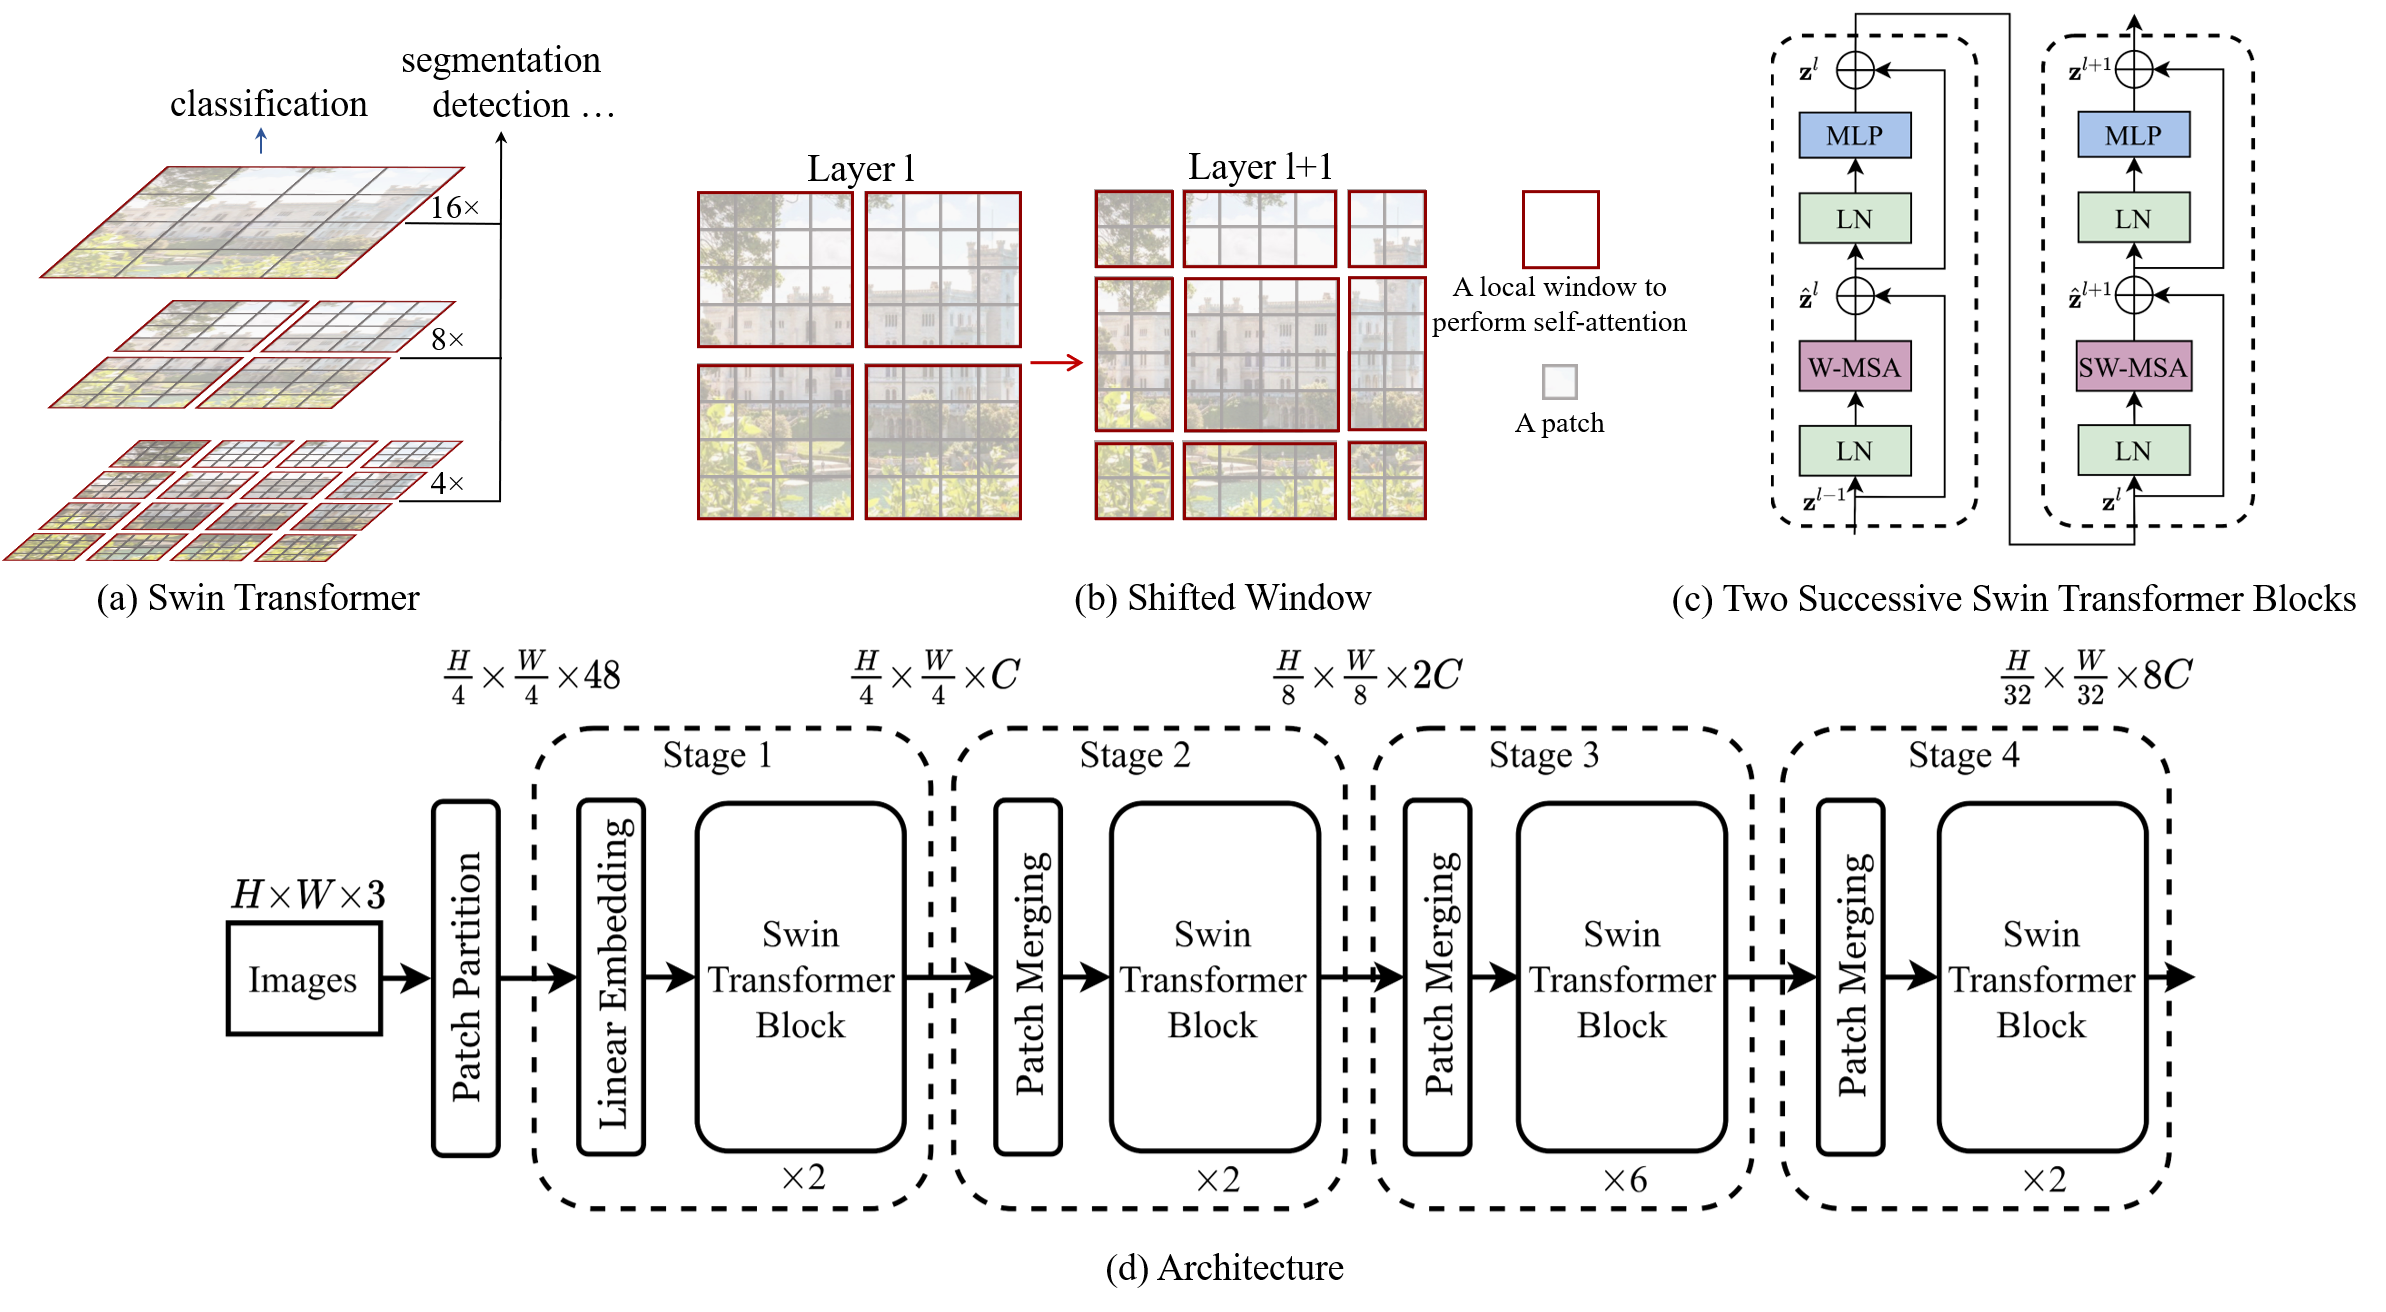
\includegraphics[width=0.9\textwidth]{img/chap3/3-2-swintransformer.png}
    \caption{Swin Transformer结构图，引用自\cite{liu2021swin}}
    \label{fig:3-2-swintransformer}
\end{figure}

如\ref{fig:3-2-swintransformer}(d)中所示，原始图像经过Patch切分后需要经过4个Stage，得到最终输出的预测值。第一个Stage由Linear Embedding和2个Swin Transformer Block组成，其余的Stage均由Patch Merging和数个Swin Transformer组成。这即是生成层次化的特征表示的过程，随着网络深度的增加，Token的数量通过斑块合并层（patch merging layers）逐渐减少，具体而言，从$\frac{H}{4}\times \frac{W}{4}\times 48$到$\frac{H}{4}\times \frac{W}{4}\times C$最终到$\frac{H}{32}\times \frac{W}{32}\times 8C$，最终实现了从整张图片中提取低维度特征的效果。对于我们的野火风险预测任务，虽然输入的不是RGB图像，而是静态变量或动态变量的组合，但原理与处理方法与之相似。

Swin Transformer Block的构建方式是将标准 Transformer 模块中的全局多头自注意力（Multi-head Self-Attetion，MSA）模块替换为基于移动窗口机制的注意力模块，同时保持其余网络层结构不变。相关架构如图\ref{fig:3-2-swintransformer}(c)所示，单个 Swin Transformer 模块包含一个基于移动窗口的多头自注意力模块，以及紧随其后的两层多层感知机（MLP），该感知机内部采用 GELU 非线性激活函数。此外，在每个自注意力模块和多层感知机之前均应用了层归一化（LN）操作，并在每个模块的输出端都加入了残差连接。

下面我们详细介绍基于移动窗口的多头自注意力模块，也是Swin Transformer架构的核心创新之处。

标准的Transformer架构及ViT\cite{dosovitskiy2020image}都进行全局自注意力计算，即计算一个token与其他所有token之间的关系，导致参数数量的二次复杂度，因此不适合需要大量token以实现密集预测或高分辨率图像的问题。为了高效建模，Swin Transformer在局部窗口内计算自注意力的值，这些窗口由图像均匀分割且不重叠。假设每个窗口包含$h\times w$个Patch，每个Patch的形状为$M\times M$，则全局MSA模块和基于窗口的MSA模块（W-MSA）的计算复杂度分别为：
\begin{equation}
    \Omega_{\text{MSA}} = 4hwC^2 + 2(hw)^2cm
\end{equation}
\begin{equation}
    \Omega_{\text{W-MSA}} = 4hwC^2 + 2M^2hwC
\end{equation}
其中前者是切片数量$hw$的二次方，而后者在M固定时的计算复杂度是线性的。

窗口的切分（window partitioning）减少了计算复杂度，但限制了不同窗口之间的连接。因此，作者提出了滑动窗口（Shifted window）多头自注意力机制，并在Swin Transformer Block中连续使用交替使用两种划分配置，即W-MSA和SW-MSA。如图\ref{fig:3-2-swintransformer}(b)所示，第一个模块采用了从左上像素开始的常规窗口划分策略，$8\times 8$的特征映射被均匀划分为$2\times 2$个窗口，窗口大小为$4\times 4(M = 4)$。接着，通过将窗口从原始位置向右下方移位$(\lfloor \frac{M}{2}\rfloor,\lfloor \frac{M}{2}\rfloor)$像素，下一模块采用了滑动窗口配置，保证了不同窗口之间信息的连接。采用滑动窗口划分方法，连续的Swin Transformer Block的计算如下：
\begin{equation}
\begin{aligned}
\hat{\mathbf{z}}^l &= \text{W-MSA}\left(\text{LN}\left(\mathbf{z}^{l-1}\right)\right) + \mathbf{z}^{l-1}, \\
\mathbf{z}^l &= \text{MLP}\left(\text{LN}\left(\hat{\mathbf{z}}^l\right)\right) + \hat{\mathbf{z}}^l, \\
\hat{\mathbf{z}}^{l+1} &= \text{SW-MSA}\left(\text{LN}\left(\mathbf{z}^l\right)\right) + \mathbf{z}^l, \\
\mathbf{z}^{l+1} &= \text{MLP}\left(\text{LN}\left(\hat{\mathbf{z}}^{l+1}\right)\right) + \hat{\mathbf{z}}^{l+1},
\end{aligned}
\end{equation}
其中$\hat{\mathbf{z}}^l$和$\mathbf{z}^l$分别表示块（Block）$l$的 （S）W-MSA 模块和 MLP 模块的输出特征。

此外，移动窗口划分机制存在一个固有缺陷，在移动配置下参与批处理的窗口总数可能会增加，且当窗口滑动时边界处会产生部分尺寸小于$M\times M$的残缺窗口。一种常规的解决方案是将这些残缺窗口零填充（pad）至标准的$M\times M$尺寸，并在计算注意力时将填充区域利用掩码（mask）剔除。然而，当常规划分下的窗口总数较少时（例如仅有$2\times 2$个窗口），这种零填充方案所带来的额外计算开销是较大的（窗口数由$2\times 2$增至$3\times 3$，计算量暴增 2.25 倍）。为此，作者提出了一种更为高效的批处理计算方法，即向左上角方向进行循环移位（cyclic-shifting)，如图\ref{fig:3-2-shifted-window}所示。经过循环移位后，一个完整的批处理窗口可能由多个在原始特征图上不相邻的子窗口拼凑而成。因此，模型引入了掩码机制（masking mechanism），以严格限制自注意力的计算仅在各个原本相邻的子窗口内部进行，保障了计算的高效性。
\begin{figure}[htbp]
    \centering
    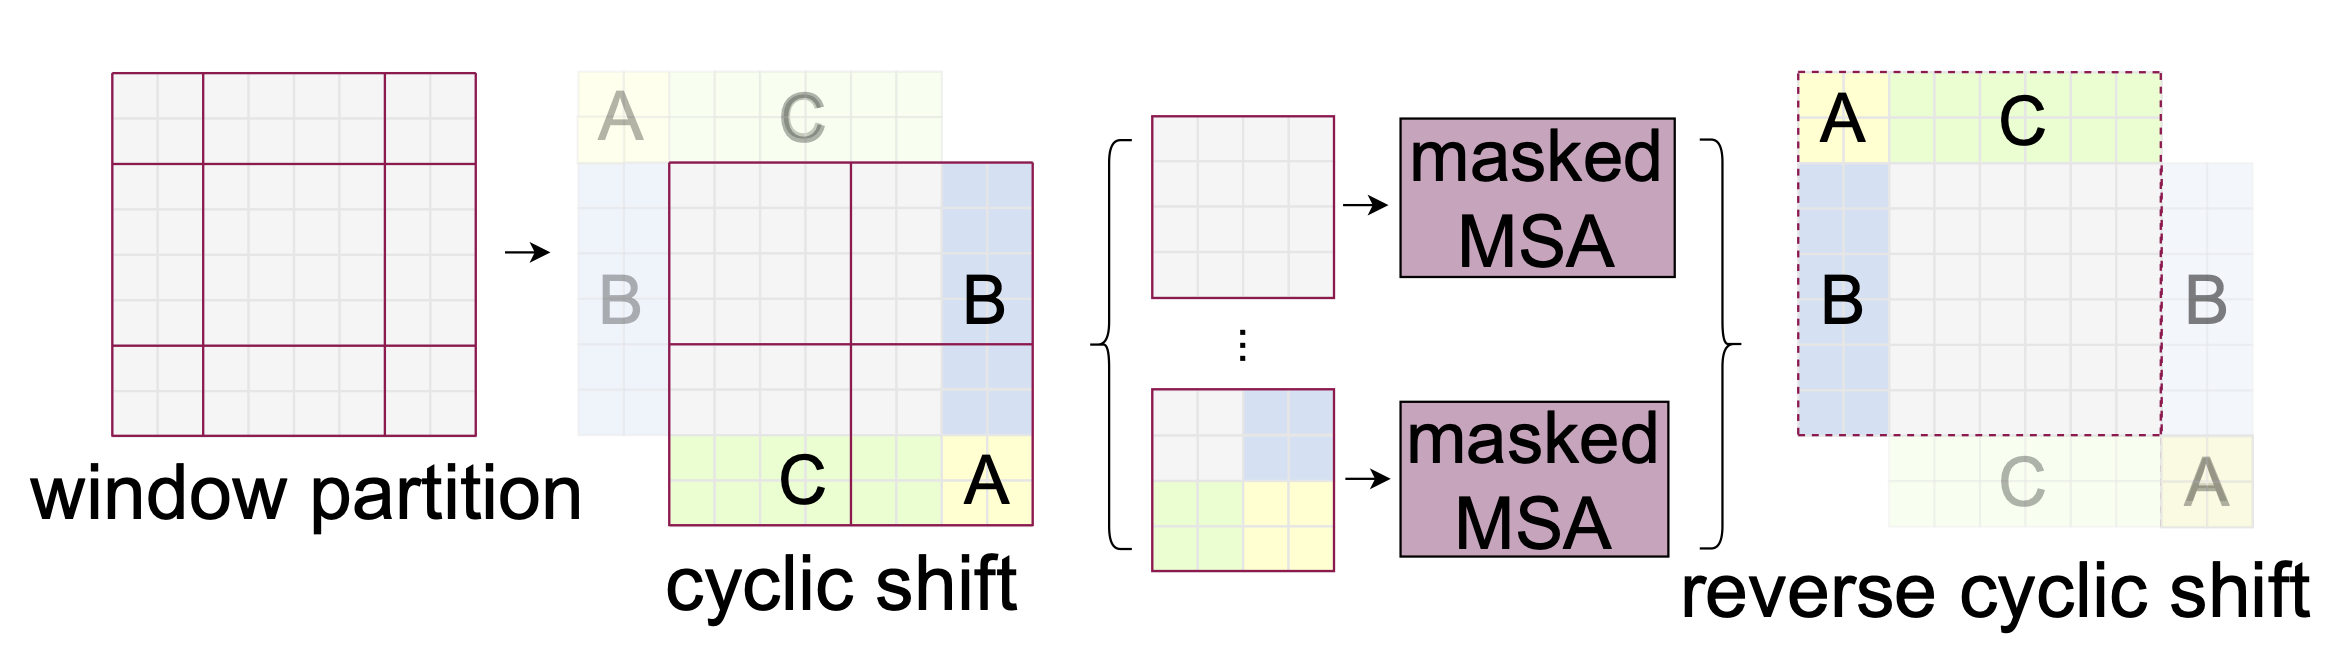
\includegraphics[width=0.9\textwidth]{img/chap3/3-2-shifted-window.png}
    \caption{移位窗口划分中高效批量计算方法的示例，引用自\cite{liu2021swin}}
    \label{fig:3-2-shifted-window}
\end{figure}
在计算自注意力时，作者未使用原始Transformer中的绝对位置编码，而是为每个头（head）引入一个相对位置偏置 $B \in \mathbb{R}^{M^2 \times M^2}$：
\begin{equation}
\text{Attention}(Q, K, V) = \text{SoftMax}(QK^T / \sqrt{d} + B)V,
\end{equation}
其中 $Q, K, V \in \mathbb{R}^{M^2 \times d}$ 分别代表查询（query）、键（key）和值（value）矩阵；$d$ 是查询矩阵和键矩阵的维度，而 $M^2$ 是单个窗口内包含的切片（patch）数量。由于沿每个坐标轴的相对位置均落在 $[-M + 1, M - 1]$ 的区间范围内，作者参数化了一个尺寸较小的偏置矩阵 $\hat{B} \in \mathbb{R}^{(2M-1) \times (2M-1)}$，而矩阵 $B$ 中的取值均直接映射自 $\hat{B}$。

\section{双分支Swin Transformer预测模型}
\label{sec:3-3}
本节主要介绍双分支特征提取网络的具体结构。在\ref{sec:3-2}节对Swin Tranformer基本原理的介绍中，我们知道其在计算机视觉尤其是图像领域有着很好的应用，而野火时空预测任务中的静态变量与动态变量组成的网格和图像的特征有异曲同工之处，因此本研究选择基于Swin Transformer搭建预测模型。为了让它能够处理野火预测任务中复杂的气象和地理数据，我们将模型拆分成了两个并行的分支：一个 3D 分支用于动态变量，另一个 2D 分支处理静态变量。

两条分支都保留了 Swin Transformer 最核心的滑动窗口注意力机制（Shifted Window Attention）和逐步下采样（Patch Merging）的结构。但为了适配具体的输入数据，我们对网络的层数、通道数和窗口大小进行了重新设置。
\subsection{气象动力学特征提取模块：Swin Transformer 3D}
\label{sec:3-3-1}

该模块负责对多变量动态气象序列进行时空联合编码。模型的输入为动态气象张量 $X_{dyn} \in \mathbb{R}^{B \times C_{in} \times D \times H \times W}$，其中批次大小为 $B$，特征通道数 $C_{in}=10$（即输入十个动态变量），时间序列长度 $D=10$，空间分辨率 $H=W=25$。

由于在本任务中输入的时空变量为三维变量，每个的特征维度为 $[10,25,25]$，共有 10 个动态变量，因此普通的 Swin Transformer 架构无法直接处理动态变量。本研究采用 Swin Transformer3D \cite{yang2025swin3d}，其与 \ref{sec:3-2} 节中介绍的基本原理类似，但将自注意力机制的作用域从二维平面拓展至了三维时空域。在常规的二维架构中，模型仅能在单一时间断面的空间窗口内捕捉静态分布，无法跨越时间步感知气象变量的物理演化。Swin Transformer 3D 的核心原理在于引入了3D Swin Transformer Block，使用三维局部窗口与三维循环移位（3D Cyclic-shifting）机制。

如图\ref{fig:3-3-swin3d}所示，模型将输入的时空张量划分为多个大小为 $(P, M, M)$ 的非重叠时空立方体，并在这些独立的三维窗口内计算自注意力。随后，网络在时间、高度和宽度三个维度上同步施加尺寸为 $(\lfloor P/2 \rfloor, \lfloor M/2 \rfloor, \lfloor M/2 \rfloor)$ 的空间错位，并结合三维掩码（Mask）机制，使得前一网络层中被物理截断的时序片段在深层网络中得以重新拼接。Swin Transformer3D提出后，被广泛应用于视频、三维体素等领域，并具有很好的效果。这一机制打破了原有结构难以处理含时变量的局限，赋予了模型强大的时域感受野，使其能够精准捕获变量的时空特征。

\begin{figure}[htbp]
    \centering
    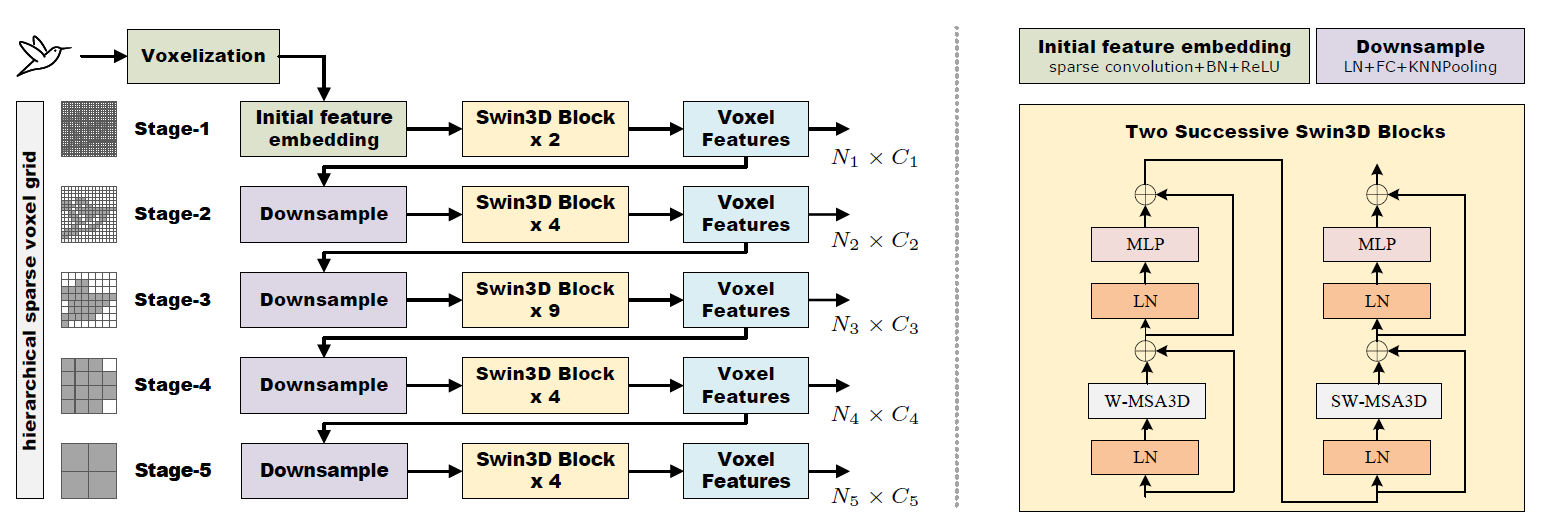
\includegraphics[width=0.9\textwidth]{img/chap3/3-3-swin3d.png}
    \caption{Swin Transformer 3D结构图，引用自\cite{yang2025swin3d}}
    \label{fig:3-3-swin3d}
\end{figure}

针对本研究所使用的小尺度野火气象数据集，本模块对标准的三维架构进行了参数适配。首先，在特征嵌入（Patch Embedding）阶段，模型利用核大小与步长均为 $(1, 1, 1)$ 的三维卷积，将跨越 10 个动态变量跨通道融合并映射至 $C=32$ 的高维特征空间。其次，在注意力窗口尺寸的设定上，模型采用了 $\mathcal{W}_{dyn}=(3, 5, 5)$ 配置。空间窗口尺寸设置为5，因为能够被输入空间边长 25 严格整除；时间窗口尺寸设置为2，也能够被时间长度10整除，意味着模型在单层前向传播中综合计算相邻2日天气波动，并能够在不同窗口之间进行连接。同时，这种设置从底层逻辑上消除了边缘零填充（Padding）所引发的边界噪声与算力消耗。

网络主体构建了包含三个阶段（Stage）的时空特征提取层，各阶段的Swin Transformer Block深度配置为 $[2, 2, 8]$，并在经过多尺度下采样后，输出维度为 $\mathbb{R}^{B \times C_{out} \times D_{out} \times H_{out} \times W_{out}}$ 的高维张量。在输出端，模块沿时间维度 $D_{out}$ 执行均值聚合（Mean Pooling）操作，将三维时空表征为二维空间特征图，从而在保留历史气候演变信息的前提下，在张量维度上方便与后续静态变量分支的特征图进行融合。具体算法可参考附录\ref{app:A-1}的DynamicSwin3D类。

\subsection{静态地貌特征编码模块：Swin Transformer 2D}
\label{sec:3-3-2}
静态变量编码分支主要负责处理不随时间变化的地理背景信息。在本研究中，输入的静态特征张量 $X_{stat} \in \mathbb{R}^{B \times C_{stat} \times H \times W}$ 是由数字高程模型（DEM）、地表坡度等地形变量与土地覆盖类型（CLC）数据拼接而成。本研究中采用的Swin Transformer2D结构及数据输入流程如下。

首先是特征嵌入（Patch Embedding）阶段。不同于原生 Swin Transformer 采用的非重叠斑块切分（Patch Splitting），本模块在输入端设计了一个由二维卷积（\texttt{Conv2d}）、批量归一化（\texttt{BatchNorm2d}）和 \texttt{GELU} 激活函数组成的序列化算子。其中，卷积核大小设为 3，填充（Padding）设为 1。这种设计使得模型在将原始静态变量映射至 $C=32$ 的隐空间时，不仅提取了平滑的局部空间过渡特征，还百分之百保留了原始的 $H \times W$ 空间分辨率，张量形状演变为 $[B, C, H, W]$。这是由于静态变量输入的尺寸为$25\times 25$，不同于RGB图像的常见尺寸$224\times 224$，较小的分辨率若再进行切分容易造成信息丢失，因此直接采用简单的卷积网络进行映射。

为了便于实现，静态变量编码模块直接复用Swin Transformer3D的结构，即在通道维度后插入一个尺寸为 1 的伪时间维度，使张量形状扩张为 $[B, C, 1, H, W]$，使得二维空间特征能够无缝对接后续的三维注意力算子。张量进入自适应局部窗口注意力（Adaptive Local Window Attention）计算时，在超参数配置上，模型将窗口尺寸约束为 $\mathcal{W}_{stat}=(1, 5, 5)$。由于张量的时间维度厚度为 1，且注意力时间窗口大小亦为 1，三维注意力机制在进行矩阵内积运算时，自然退化为纯粹的二维局部空间注意力。考虑到地形特征的语义相对直观，该模块的网络深度被轻量化配置为 $[2, 2]$，即仅包含一次斑块合并（Patch Merging）下采样操作。

最后执行通道投影与空间对齐（Channel Projection \& Spatial Alignment）。在完成两个阶段的前向传播后，模块首先通过 \texttt{squeeze(2)} 操作剥离冗余的伪时间维度，使张量回归二维物理空间。随后，利用 $1 \times 1$ 卷积层（\texttt{proj}）进行跨通道信息交融，将特征维度映射至目标维度。为了消除浅层下采样带来的分辨率差异，模块在输出端应用了自适应二维平均池化层（\texttt{AdaptiveAvgPool2d}），将特征图的几何分辨率对齐至目标尺寸。这一系列操作确保了静态地貌表征与动态气象表征在通道与空间尺寸上的同构，为后续的特征融合奠定了基础。具体算法可参考附录\ref{app:A-1}的StaticSwin2D类。

\section{特征融合模块：地理感知交叉注意力机制（Geographic Cross-Attention）}
\label{sec:3-4}
在完成双分支特征提取后，模型分别获得了蕴含历史气象演变规律的动态特征图 $\mathcal{F}_{dyn} \in \mathbb{R}^{B \times C \times H \times W}$ 与蕴含地形地貌先验的静态特征图 $\mathcal{F}_{stat} \in \mathbb{R}^{B \times C \times H \times W}$。为了实现两种特征的深度耦合，本研究设计了一种地理感知交叉注意力机制（Geographic Cross-Attention, Geo-CA）。相比于简单的特征拼接或传统的全局注意力，Geo-CA 能够以显式的方式注入空间几何约束，引导模型关注物理意义上更相关的局部区域。

Geo-CA 模块的核心逻辑是利用当前的气象状态（即动态特征图）去检索与之相关的地理环境（即静态特征图）。在计算过程中，动态气象特征 $\mathcal{F}_{dyn}$ 经过线性映射生成查询矩阵（Query, $Q$），而静态地貌特征 $\mathcal{F}_{stat}$ 则生成键矩阵（Key, $K$）与值矩阵（Value, $V$）。

设特征图展平后的 Token 序列为 $N = H \times W$，则标准交叉注意力的计算公式为：
\begin{equation}
    \text{Attention}(Q, K, V) = \text{SoftMax}\left(\frac{QK^T}{\sqrt{d_k}}\right)V
\end{equation}
其中 $d_k$ 为特征维度缩放因子。在这种模式下，模型能够根据当前气象条件，自适应地学习不同地形因素对野火蔓延的影响程度。

然而，传统注意力机制通常采用全局建模方式，对所有空间位置赋予相同的建模能力，这与野火蔓延的实际规律并不完全一致。野火传播本质上具有明显的局部扩散特征，即距离中心区域越近的地理环境，对当前位置起火风险的影响往往越显著。为了增强模型对这种空间局部性的表达能力，本研究在注意力得分中引入地理距离约束。

具体而言，模型首先根据输入特征图的空间尺寸构建欧氏距离矩阵。设空间中任意两个像素点 $i$ 和 $j$ 的归一化坐标分别为 $(x_i, y_i)$ 与 $(x_j, y_j)$，其相对空间向量为 $(\Delta x_{ij}, \Delta y_{ij}) = (x_i - x_j, y_i - y_j)$。两者之间的欧氏距离计算如下：
\begin{equation}
    dist_{i,j} = \sqrt{(x_i - x_j)^2 + (y_i - y_j)^2}
\end{equation}

在此基础上，引入可学习的地理衰减参数 $\tau$，用于控制距离约束的强度。为保证距离惩罚始终为正，并满足“距离越远、影响越弱”的物理直觉，本文通过 $\text{softplus}(x)=ln(1+e^x)$ 函数对参数进行约束。最终，地理感知交叉注意力的得分矩阵 $\mathbf{A}$ 可表示为：
\begin{equation}
    \mathbf{A}_{i,j} = \frac{Q_i K_j^T}{\sqrt{d_k}} - \text{softplus}(\tau) \cdot dist_{i,j}
\end{equation}

其中，第二项为空间距离惩罚项，用于抑制远距离区域之间的注意力权重。通过该设计，模型能够更加关注中心区域附近的地形特征与可燃物分布，从而更符合野火蔓延的局部传播规律。同时，$\tau$ 为可学习参数，模型可以根据不同区域及不同火灾场景，自适应调整空间约束强度。

基于上述设计的地理感知交叉注意力机制，不仅实现了静态地理变量与动态气象变量之间的有效融合，同时增强了模型对局部野火传播模式的建模能力。具体算法可参考附录\ref{app:A-2}的GeoCrossAttention类。

\section{物理信息启发的数据重构与注意力偏置}
\label{sec:3-5}
在时空预测任务中，完全依赖数据驱动的深度学习模型，往往难以有效学习复杂环境中的非线性物理规律。为提升模型对极端火险条件的感知能力，本文提出一种基于物理信息启发（Physics-Informed）的特征重构策略，通过引入具有明确物理意义的气象变量，将领域知识融入模型输入过程。本节主要介绍饱和水汽压差（VPD）特征的构建方法，以及基于风场信息的注意力偏置机制。

\subsection{基于热力学先验的饱和水汽压差（VPD）特征重构}
\label{sec:3-5-1}
相比原始气温（t2m）与露点温度（d2m），VPD 与火灾风险之间具有更直接的物理联系。然而，VPD 与温度之间存在明显的非线性关系，神经网络难以仅依赖原始变量自动学习这一复杂映射。因此，本文基于热力学理论显式构建 VPD 特征，并将其作为新增动态变量输入模型。

在引入 VPD（之前，我们从基础热力学出发，推导其与原始温度变量（气温 $t$ 与露点温度 $t_d$）之间的数学关系。在热力学平衡条件下，液态水与水汽的比吉布斯自由能满足$g_v = g_l$。结合热力学基本微分方程 $dg = -s dT + \alpha de_s$ ，当系统沿平衡曲线发生微小状态变化时，其比熵 $s$ 与比容 $\alpha$ 满足以下关系：
\begin{equation}
    -s_v dT + \alpha_v de_s = -s_l dT + \alpha_l de_s
\end{equation}
引入相变潜热定律 $L_v = T(s_v - s_l)$，通过移项整理，即可得到描述相变过程核心规律的\textbf{克劳修斯-克拉珀龙方程（Clausius-Clapeyron equation）}：
\begin{equation}
    \frac{de_s}{dT} = \frac{L_v}{T(\alpha_v - \alpha_l)}
\end{equation}
该公式定义了饱和水汽压 $e_s$ 随绝对温度 $T$ 变化的斜率。

为了将该理论方程应用于真实大气环境，我们引入两项关键的近似：首先，水汽的比容远大于液态水的比容（$\alpha_v \gg \alpha_l$），故分母可简化为 $T \alpha_v$；其次，将水汽视为理想气体，满足状态方程 $\alpha_v = R_v T / e_s$（其中 $R_v$ 为水汽气体常数）。将上述两项代入式 (1)，得到水汽专用的微分方程形式：
\begin{equation}
    \frac{de_s}{dT} = \frac{L_v e_s}{R_v T^2}
\end{equation}

通过分离变量法对式 (2) 进行积分。我们选取水的三相点（温度 $T_0 = 273.15 \text{ K}$，对应的饱和水汽压 $e_{s0} = 6.11 \text{ hPa}$）作为积分下限，并假设在常规气象温度范围内汽化潜热 $L_v$ 为常数，积分结果如下：
\begin{equation}
    \ln\left(\frac{e_s}{e_{s0}}\right) = \frac{L_v}{R_v} \left( \frac{1}{T_0} - \frac{1}{T} \right) = \frac{L_v}{R_v} \left( \frac{T - T_0}{T_0 T} \right)
\end{equation}

随后，将绝对温度转换为摄氏温度。并且，为了弥补先前积分过程中“潜热 $L_v$ 为常数”以及“水汽为绝对理想气体”等假设所带来的理论误差，学者利用大量精密实验数据对该公式的理论常数进行了修正，最终得到了气象学中广泛使用的\textbf{马格努斯-泰登（Magnus-Tetens）经验公式}\cite{murray1967computation}：
\begin{equation}
    e_s(t) = 0.611 \times \exp\left(\frac{17.27 \times t}{t + 237.3}\right)
\end{equation}
式中，常数 17.27 与 237.3 即为实验拟合所得的修正参数，压强单位为 kPa。

至此，饱和水汽压 $e_s$ 与环境气温 $t$ 的关系得以确定。基于上述理论，野火动力学中的核心变量 VPD 可被定义为当前气温下的饱和水汽压 $e_s(t)$ 与由露点温度 $t_d$ 决定的实际水汽压 $e_a(t_d)$ 之差：
\begin{equation}
    VPD = 0.611 \times \left[ \exp\left(\frac{17.27 \times t}{t + 237.3}\right) - \exp\left(\frac{17.27 \times t_d}{t_d + 237.3}\right) \right]
\end{equation}
本研究通过将该结果作为特征，即将VPD视为新增的动态变量，输入神经网络，从而使模型能更好地捕捉大气环境、地表水分等特征，提升了模型对野火天气的感知能力。

\subsection{风场矢量作为动力学偏置注入注意力网络}
\label{sec:3-5-2}

在具体的算法实现中，本研究将$era5\_max\_wind\_v10$和$era5\_max\_wind\_u10$，即最大经向风速和最大纬向风速，也视为特征变量，并将风场矢量在注意力分数计算的底层作为加法偏置（Additive Bias）进行注入。

设 $\mathcal{F}_{dyn}$ 为动态气象特征，在自注意力计算过程中，模型针对特征图展平后的任意查询（Query）网格 $i$ 与键（Key）网格 $j$，动态构建相对空间坐标向量 $\Delta \vec{r}_{ij} = (\Delta x_{ij}, \Delta y_{ij})$。同时，从当前时间步的气象输入中提取网格 $i$ 所处的局部风场矢量 $\vec{W}_i = (U_i, -V_i)$。由于图像矩阵的索引坐标系以向南为正向，而气象学风场标量中 $V$ 分量以向北为正向，公式中对 $V_i$ 取负号以实现两套物理坐标系的对齐。

风场动力学偏置矩阵 $\mathbf{B}_{wind}$ 的物理本质为风场矢量与空间向量的点积：
\begin{equation}
    \mathbf{B}_{wind}^{i,j} = \vec{W}_i \cdot \Delta \vec{r}_{ij} = U_i \cdot \Delta x_{ij} + (-V_i) \cdot \Delta y_{ij}
\end{equation}

该点积操作具有以下的物理可解释性：当网格 $j$ 位于网格 $i$ 的下风向（顺风）时，空间向量与风场矢量的夹角呈锐角，点积 $\mathbf{B}_{wind}^{i,j} > 0$；反之，若位于上风向（逆风），点积 $\mathbf{B}_{wind}^{i,j} < 0$。随后，该偏置项被叠加至原始的缩放点积注意力得分矩阵 $\mathbf{A}$ 之上，并与地理距离惩罚项共同作用：
\begin{equation}
    \mathbf{A}_{i,j}' = \mathbf{A}_{i,j} + \text{softplus}(\omega) \cdot \mathbf{B}_{wind}^{i,j} - \text{softplus}(\tau) \cdot dist_{i,j}
\end{equation}

其中，$dist_{i,j}$ 为两网格间的欧氏距离，$\omega$ 与 $\tau$ 分别为模型自适应学习的风场拉伸系数与地理衰减系数，两者均由 $\text{softplus}$ 函数包裹以确保参数值恒定为正。经过该物理公式重构后，注意力矩阵在进行 Softmax 归一化时，高权重区域会自发向顺风方向发生非对称性变化，而在逆风方向受到抑制。这种在深度学习底层算子中硬编码风向矢量的设计，使网络摆脱了传统注意力机制的各向同性局限。具体算法在附录\ref{app:A-2}的GeoCrossAttention类中实现。

经过上述模块的提取与耦合，网络最终输出融合了动态与静态变量的特征图。在分类输出末端，模型采用全局平均池化（Global Average Pooling）机制，沿特征图的空间维度将其压缩浓缩为一维特征向量，随后输入多层感知机（MLP），即可输出野火发生的二分类概率。至此，本架构完成了从双分支特征编码、物理先验注入到最终概率预测的完整闭环。

综上所述，本章详细介绍了应用于野火风险预测任务的模型架构设计，即物理信息启发的基于Swin Transformer的模型，通过双分支网络分别处理静态变量和动态变量，并使用地理感知交叉注意力机制进行融合，以及通过对火灾发生的动力学洞察，将物理信息作为先验注入，使模型能够同时捕捉多种特征，保证了其预测野火风险的精度。

    \chapter{实验结果与评估}
\label{chap:4}
本章主要对第三章提出的模型，即融合物理信息的基于Swin Transformer双分支预测模型，进行实验验证与性能评估。首先介绍实验的数据集划分策略、硬件环境与超参数设置；其次通过合理的评价指标验证模型在野火预测任务上的整体表现；最后，通过消融实验（Ablation Study）深入剖析各核心物理模块的有效性。
\section{数据集预处理及实验设置}
\label{sec:4-1}
考虑到野火发生具有强烈的季节性与气候周期性规律，为避免未来数据泄露到历史训练中，本实验参考\cite{loan}，采用基于时间序列的划分准则。将数据集中 2019 年之前的历史火灾与非火灾样本划分为训练集（Training Set），用于模型参数的优化；2019 年的全年样本作为验证集（Validation Set），用于监控训练过程并进行早停（Early Stopping）等决策；2020 年与 2021 年的数据作为相互独立的测试集（Test Set），用于评估模型在未知未来年份上的泛化性能。

在数据输入网络前，对所有连续型气象特征执行了全局最大最小值归一化（Min-Max Normalization），将其线性映射至 $[0, 1]$ 区间，以消除不同气象要素（如风速、温度）量纲差异对梯度反向传播的干扰。针对真实遥感与气象数据中存在的异常或缺失值，采用零填充策略处理。同时，设定动态气象变量的时间窗口步长为 10 天，即模型基于起火日前连续 10 天的气象序列进行预测。

本研究的所有深度学习模型均基于 PyTorch（2.5.1 版本）框架开发。在硬件配置方面，模型的训练与推理计算使用2张NVIDIA GeForce RTX 4080（32GB显存）。

由于本任务属于正负样本不平衡的时空二分类问题，因此在训练集加载阶段启用了数据增强（Data Augmentation）机制，如水平翻转和垂直翻转等，以扩充样本多样性，并保持正负样本比例为1：2\cite{loan}。在损失函数与激活函数的选取上，本实验在分类头末端采用 LogSoftmax 激活函数将输出映射为对数概率，并选用加权负对数似然损失函数（Weighted NLLLoss）进行模型优化。考虑到模型训练初期的梯度稳定性，本研究在基线训练阶段对非火灾样本（负类）与火灾样本（正类）赋予了均等的损失权重（$[0.5, 0.5]$），以确保模型优先学习大尺度下的基础时空气象映射规律。

在优化算法方面，选用适配 Transformer 架构的 AdamW 优化器，以利用其权重衰减（Weight Decay）特性防止过拟合，半权重衰减系数设定为 0.03，并结合丢弃率（Dropout Rate）为 0.3 的随机失活策略。初始学习率设定为 $3 \times 10^{-5}$，并配合阶梯式学习率调度策略（StepLR），每 12 个 Epoch 将学习率衰减至原来的 10\%，使模型在训练后期能够持续梯度下降。模型训练的批次大小（Batch Size）设定为 256，总训练轮次（Epoch）设定为 40 轮。

\section{实验设置与评价指标}
\label{sec:4-2}

\subsection{实验组别设置}
为了验证本研究\ref{sec:3-5}提出的物理启发——基于热力学先验的饱和水汽压差和风场矢量作为动力学偏置注入注意力网络——在野火预测任务中的有效性，设计了以下四组对比实验：

\begin{enumerate}
    \item[(1)] \textbf{基础双分支网络 (Baseline)}：剥离物理先验模块，使用动态气象特征与静态地貌特征输入 2D/3D Swin Transformer 双分支网络进行特征提取与分类。
    \item[(2)] \textbf{引入热力学特征的网络 (+VPD)}：在 Baseline 的基础上，利用马格努斯-泰登经验公式将基础气象数据重构为饱和水汽压差（VPD），也作为动态变量输入网络，以强化模型对火灾易发干旱环境的感知。
    \item[(3)] \textbf{引入动力学偏置的网络 (+UV)}：在 Baseline 的基础上，在特征融合阶段的地理感知交叉注意力机制（Geo-CA）中，将风场的经向速度 U、纬向速度V分量作为空间偏置（Spatial Bias）注入网络，引导模型关注风向带来的火势蔓延趋势。
    \item[(4)] \textbf{物理融合网络 ( +VPD \& +UV)}：本研究提出的最终模型架构，同时融合 VPD 热力学特征重构与 Geo-CA 风场动力学偏置，实现物理信息与数据驱动的深度结合。
\end{enumerate}
\subsection{评估指标}
野火预测本质上是基于极度不平衡数据的时空二分类任务。为全面客观地评估模型的性能，本实验按照前述研究的评估方法\cite{loan,dacsa,kondylatos2022wildfire}，引入混淆矩阵（Confusion Matrix），包括真正例（TP, True Positive）、假正例（FP, False Positive）、真负例（TN, True Negative）和假负例（FN, False Negative）。在此基础上，选取五项评价指标：

\begin{itemize}
    \item \textbf{精确率 (Precision)}：在模型所有预测为有火的样本中，真正有火的比例。体现了预测的准度，数值越高代表误报率越低。
    $$ Precision = \frac{TP}{TP + FP} $$
    
    \item \textbf{召回率 (Recall)}：在实际真正有火的样本中，模型成功预测出来的比例。体现了预测的全度，数值越高代表漏报率越低。在野火防灾业务中，漏报的代价远高于误报，因此该指标极具参考价值。
    $$ Recall = \frac{TP}{TP + FN} $$
    
    \item \textbf{F1 分数 (F1-Score)}：精确率与召回率的调和平均数。由于野火非着火背景极多，F1-Score 能够更好地衡量模型的综合性能。
    $$ F1\text{-}Score = 2 \times \frac{Precision \times Recall}{Precision + Recall} $$
    
    \item \textbf{AUROC (Area Under the ROC Curve)}：指受试者工作特征曲线（ROC）下的面积。它衡量了模型在不同分类判定阈值下，区分正负样本的综合能力，数值越接近 1 代表模型的区分能力越强。在数学上等价于，模型随机抽取一个正样本和负样本，正样本的预测概率排在负样本之前的概率：
    $$ AUROC = \frac{\sum_{i \in \mathcal{P}} \sum_{j \in \mathcal{N}} \mathbb{I}(p_i > p_j)}{|\mathcal{P}| \times |\mathcal{N}|} $$
    其中，$\mathcal{P}$ 和 $\mathcal{N}$ 分别为真实的正类（有火）与负类（无火）样本集合，$p_i$ 与 $p_j$ 代表模型输出的预测概率，$\mathbb{I}(\cdot)$ 为指示函数，当括号内条件成立时，指示函数值为 1，否则为 0。该公式证明了 AUROC 不受极端正负样本比例失衡的影响，也是评估野火预测模型的关键指标。
    \item \textbf{总体准确率 (Overall Accuracy, OA)}：模型正确预测的样本（含正类与负类）占总样本的比例，反映模型的整体预测正确度。
    $$ OA = \frac{TP + TN}{TP + TN + FP + FN} $$
    
\end{itemize}

\subsection{模型训练与收敛性验证}
为验证模型在训练过程中的稳定性，图\ref{fig:4-2-train_val_loss}展示了模型在训练集与验证集上的损失（Loss）演变曲线，分别是基础模型与加入不同物理信息启发的模型。可以看出，随着迭代轮次（Epoch）的增加，训练集与验证集的损失曲线在前期快速下降，之后逐渐进入平稳收敛区。
\begin{figure}[htbp]
    \centering
    % 左图：Loss 曲线
    \begin{minipage}{0.48\textwidth}
        \centering
        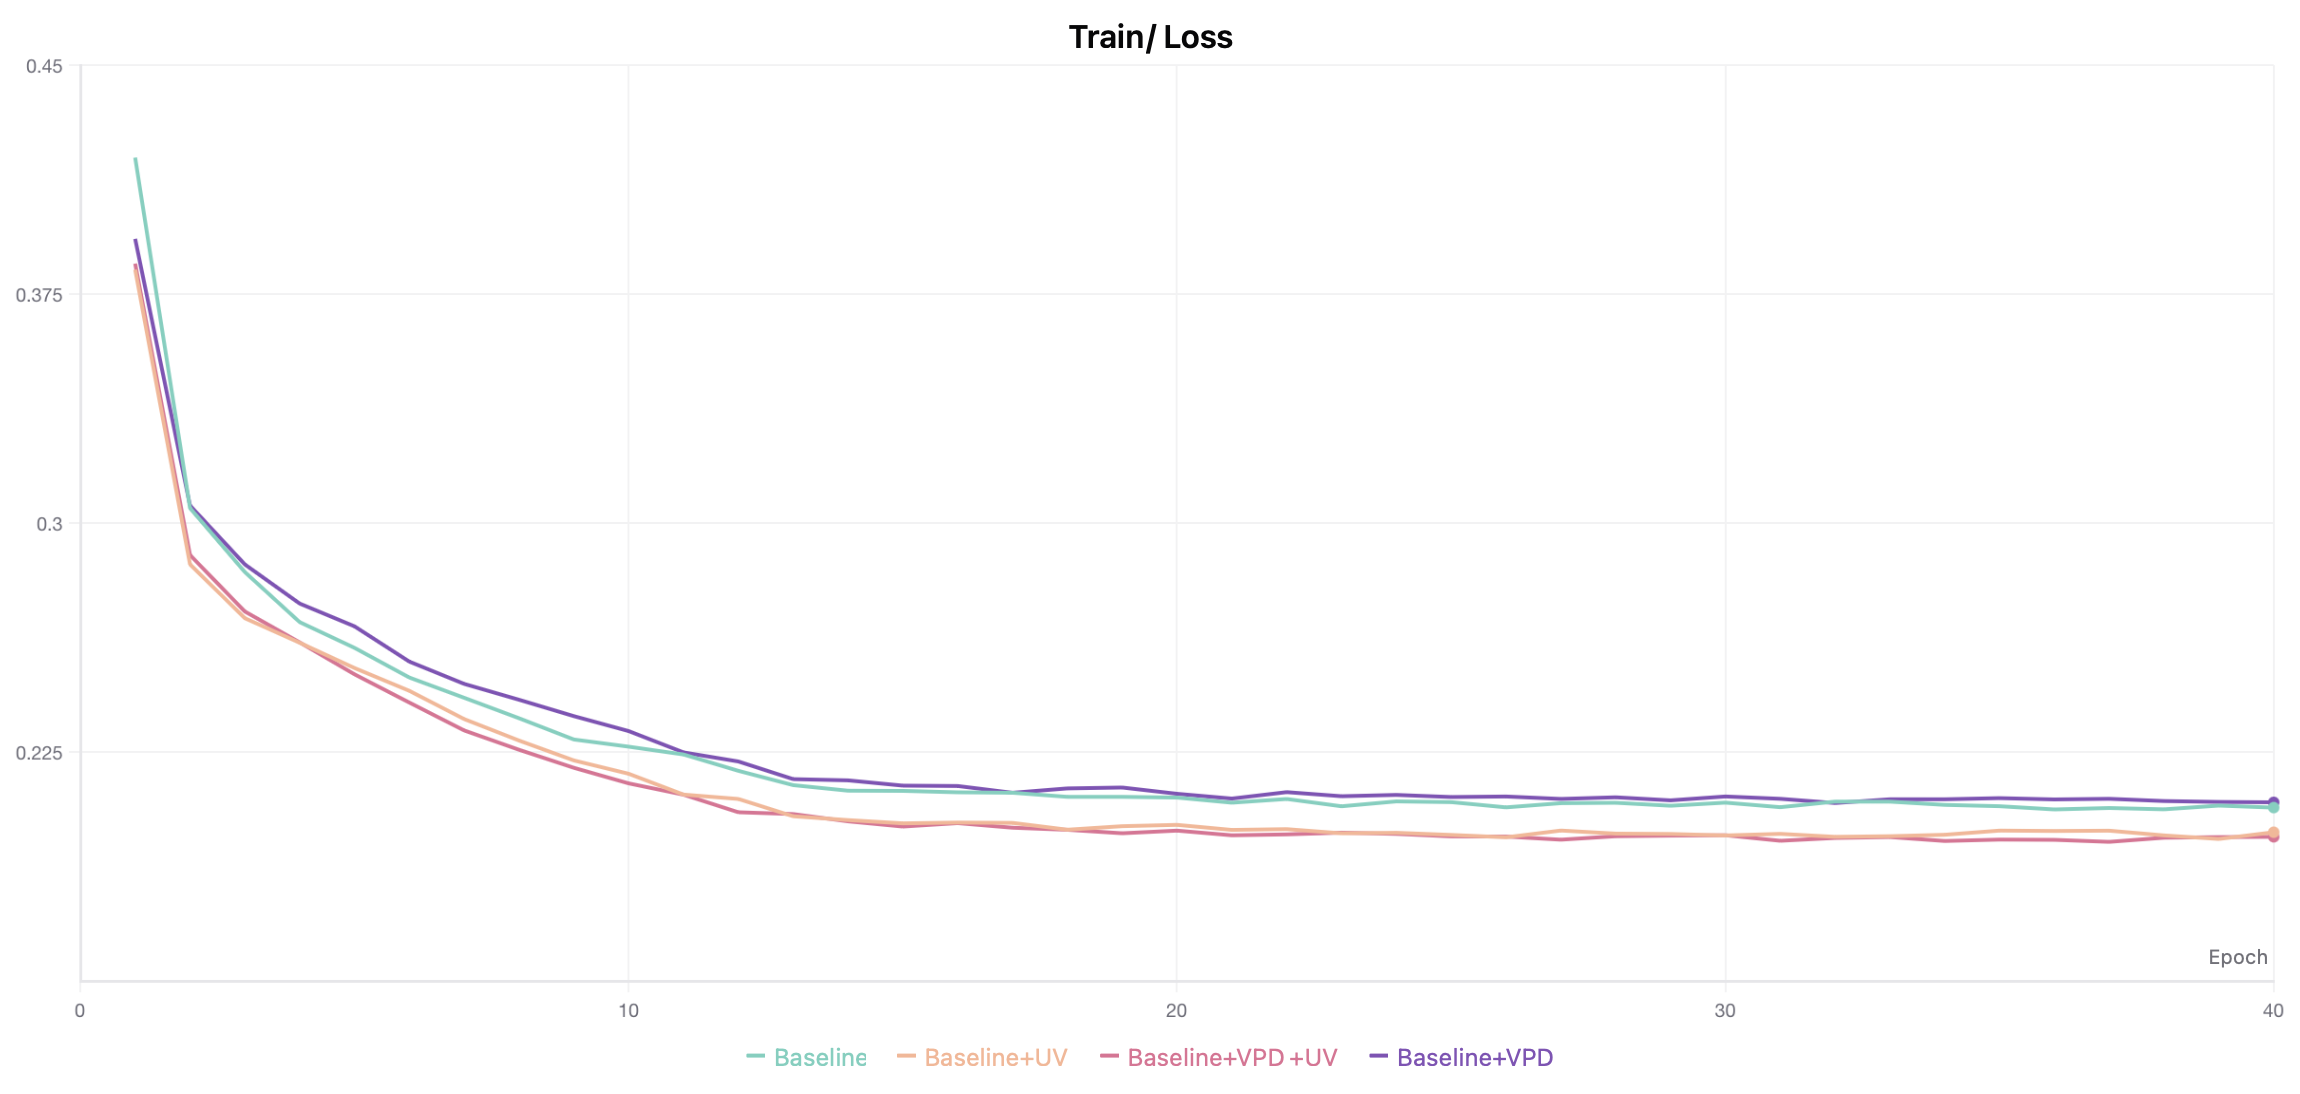
\includegraphics[width=\linewidth]{img/chap4/4-2-train-loss.png} 
        \centerline{(a) 训练集 Loss 曲线}
    \end{minipage}\hfill
    % 右图：Precision 曲线
    \begin{minipage}{0.48\textwidth}
        \centering
        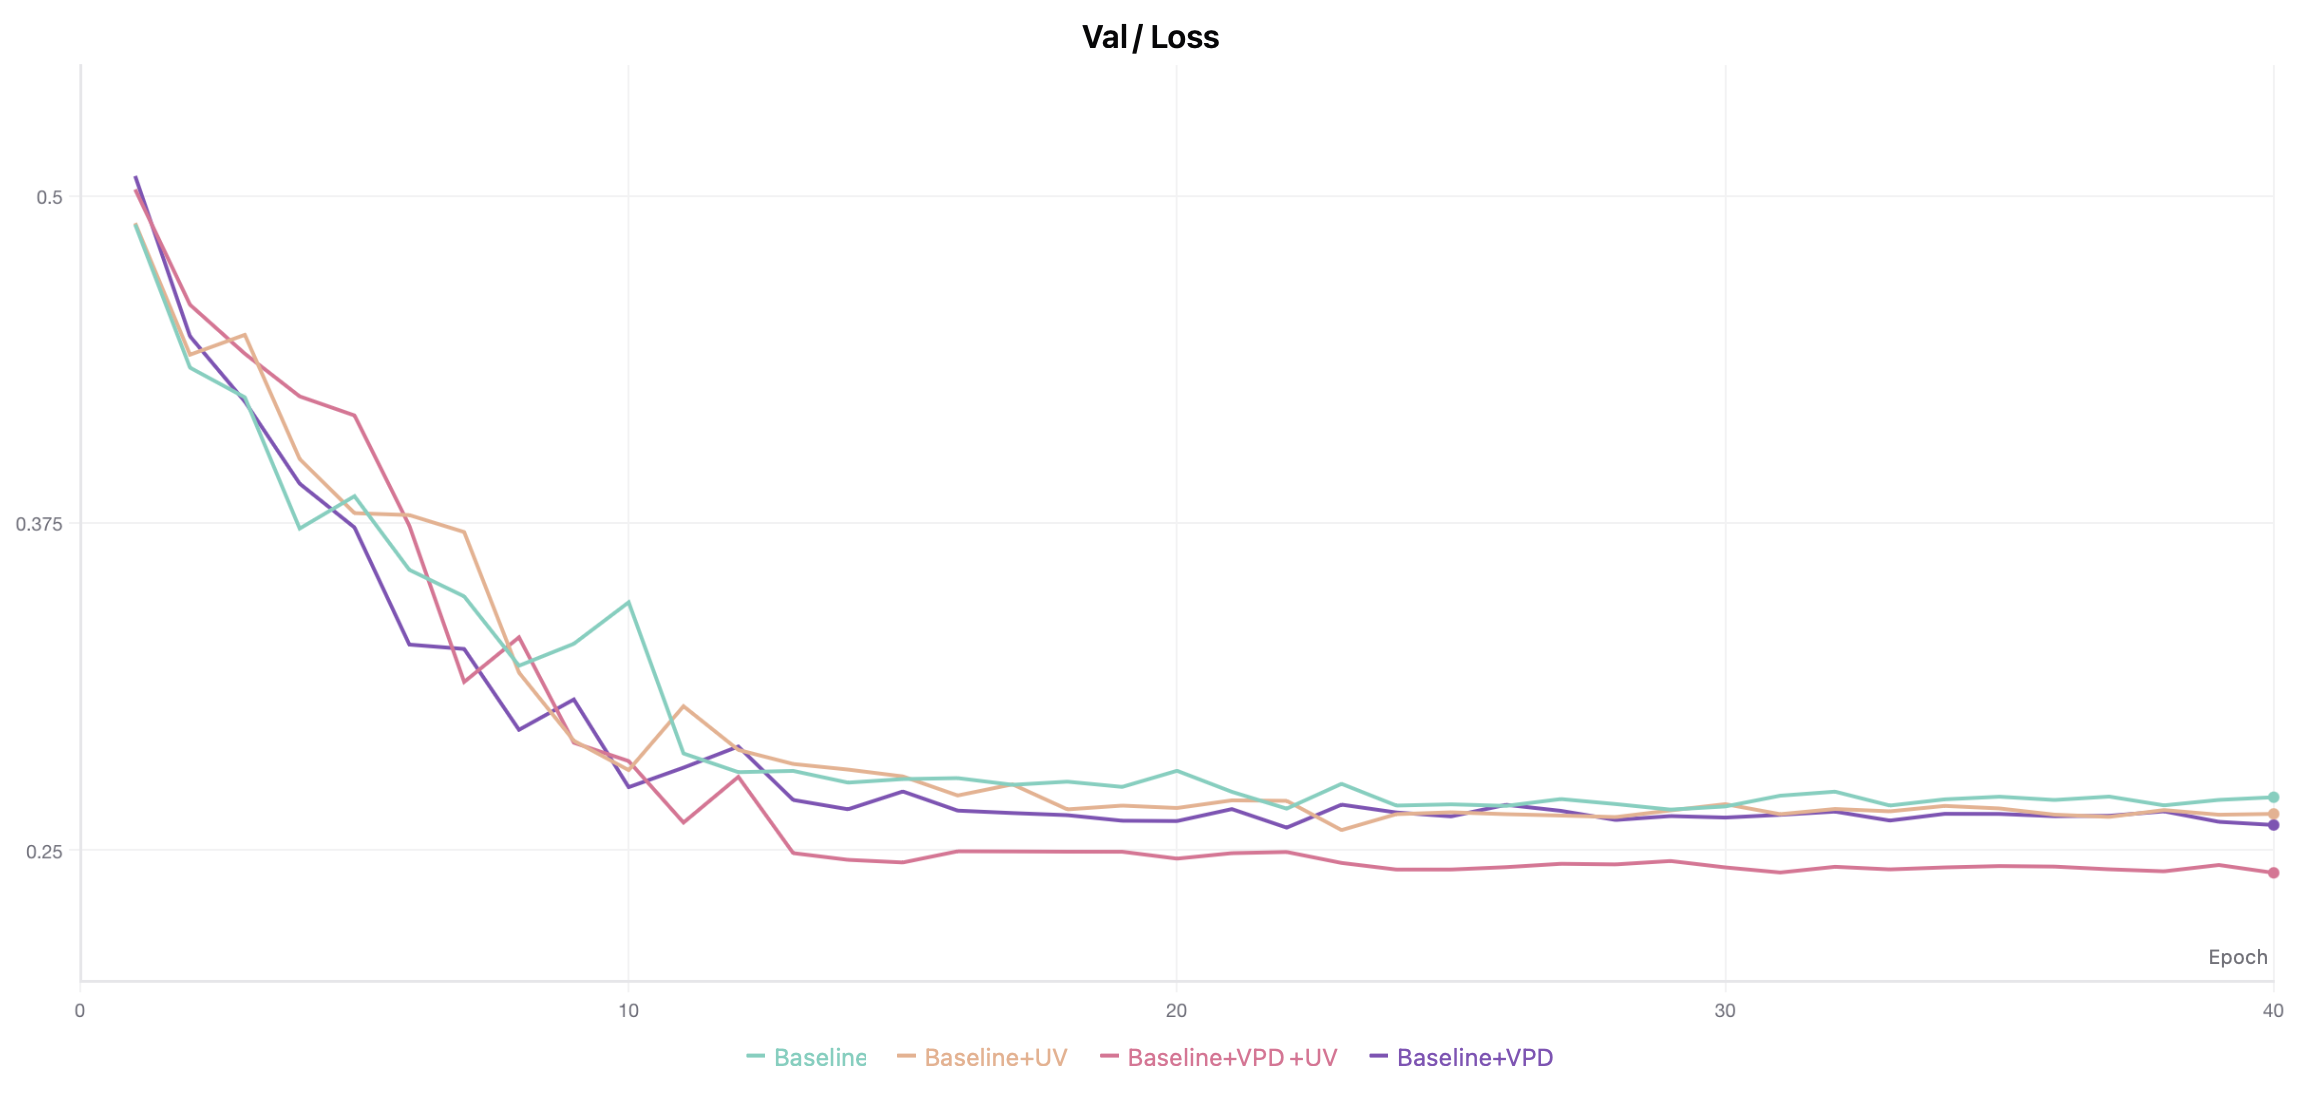
\includegraphics[width=\linewidth]{img/chap4/4-2-val-loss.png} % 替换为你的precision图路径
        \centerline{(b) 验证集 Loss 曲线}
    \end{minipage}
    \caption{模型训练过程中的Loss曲线}
    \label{fig:4-2-train_val_loss}
\end{figure}

同时，图 \ref{fig:4-2-train_val_precision}展示了模型训练过程中的精确率（Precision）曲线，表明模型的查准能力随着训练得到稳步提升，最终收敛于高置信度区间。
\begin{figure}[htbp]
    \centering
    \begin{minipage}{0.48\textwidth}
        \centering
        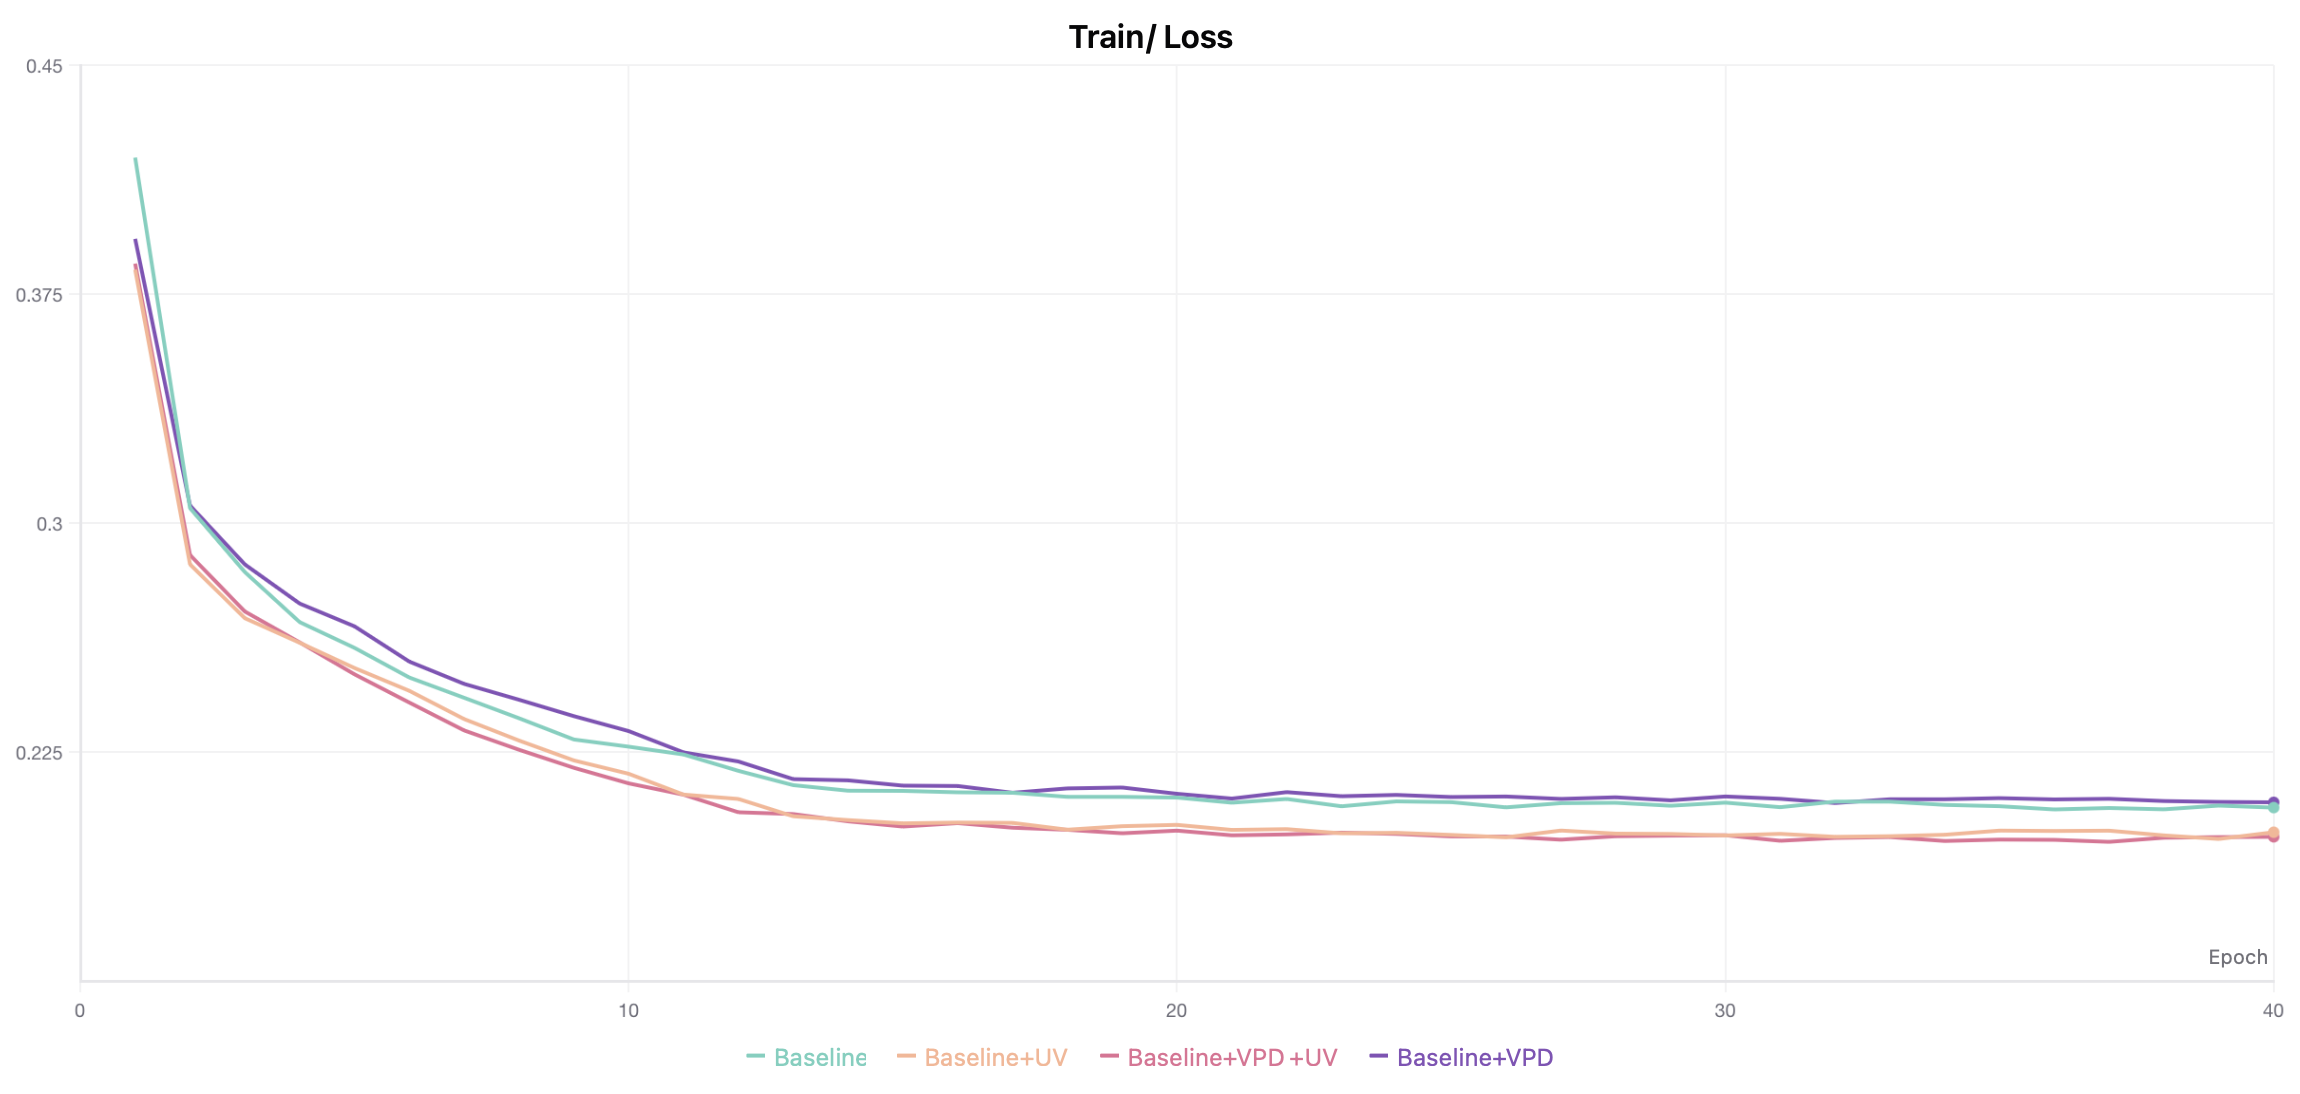
\includegraphics[width=\linewidth]{img/chap4/4-2-train-loss.png} 
        \centerline{(a) 训练集 Precision 曲线}
    \end{minipage}\hfill
    \begin{minipage}{0.48\textwidth}
        \centering
        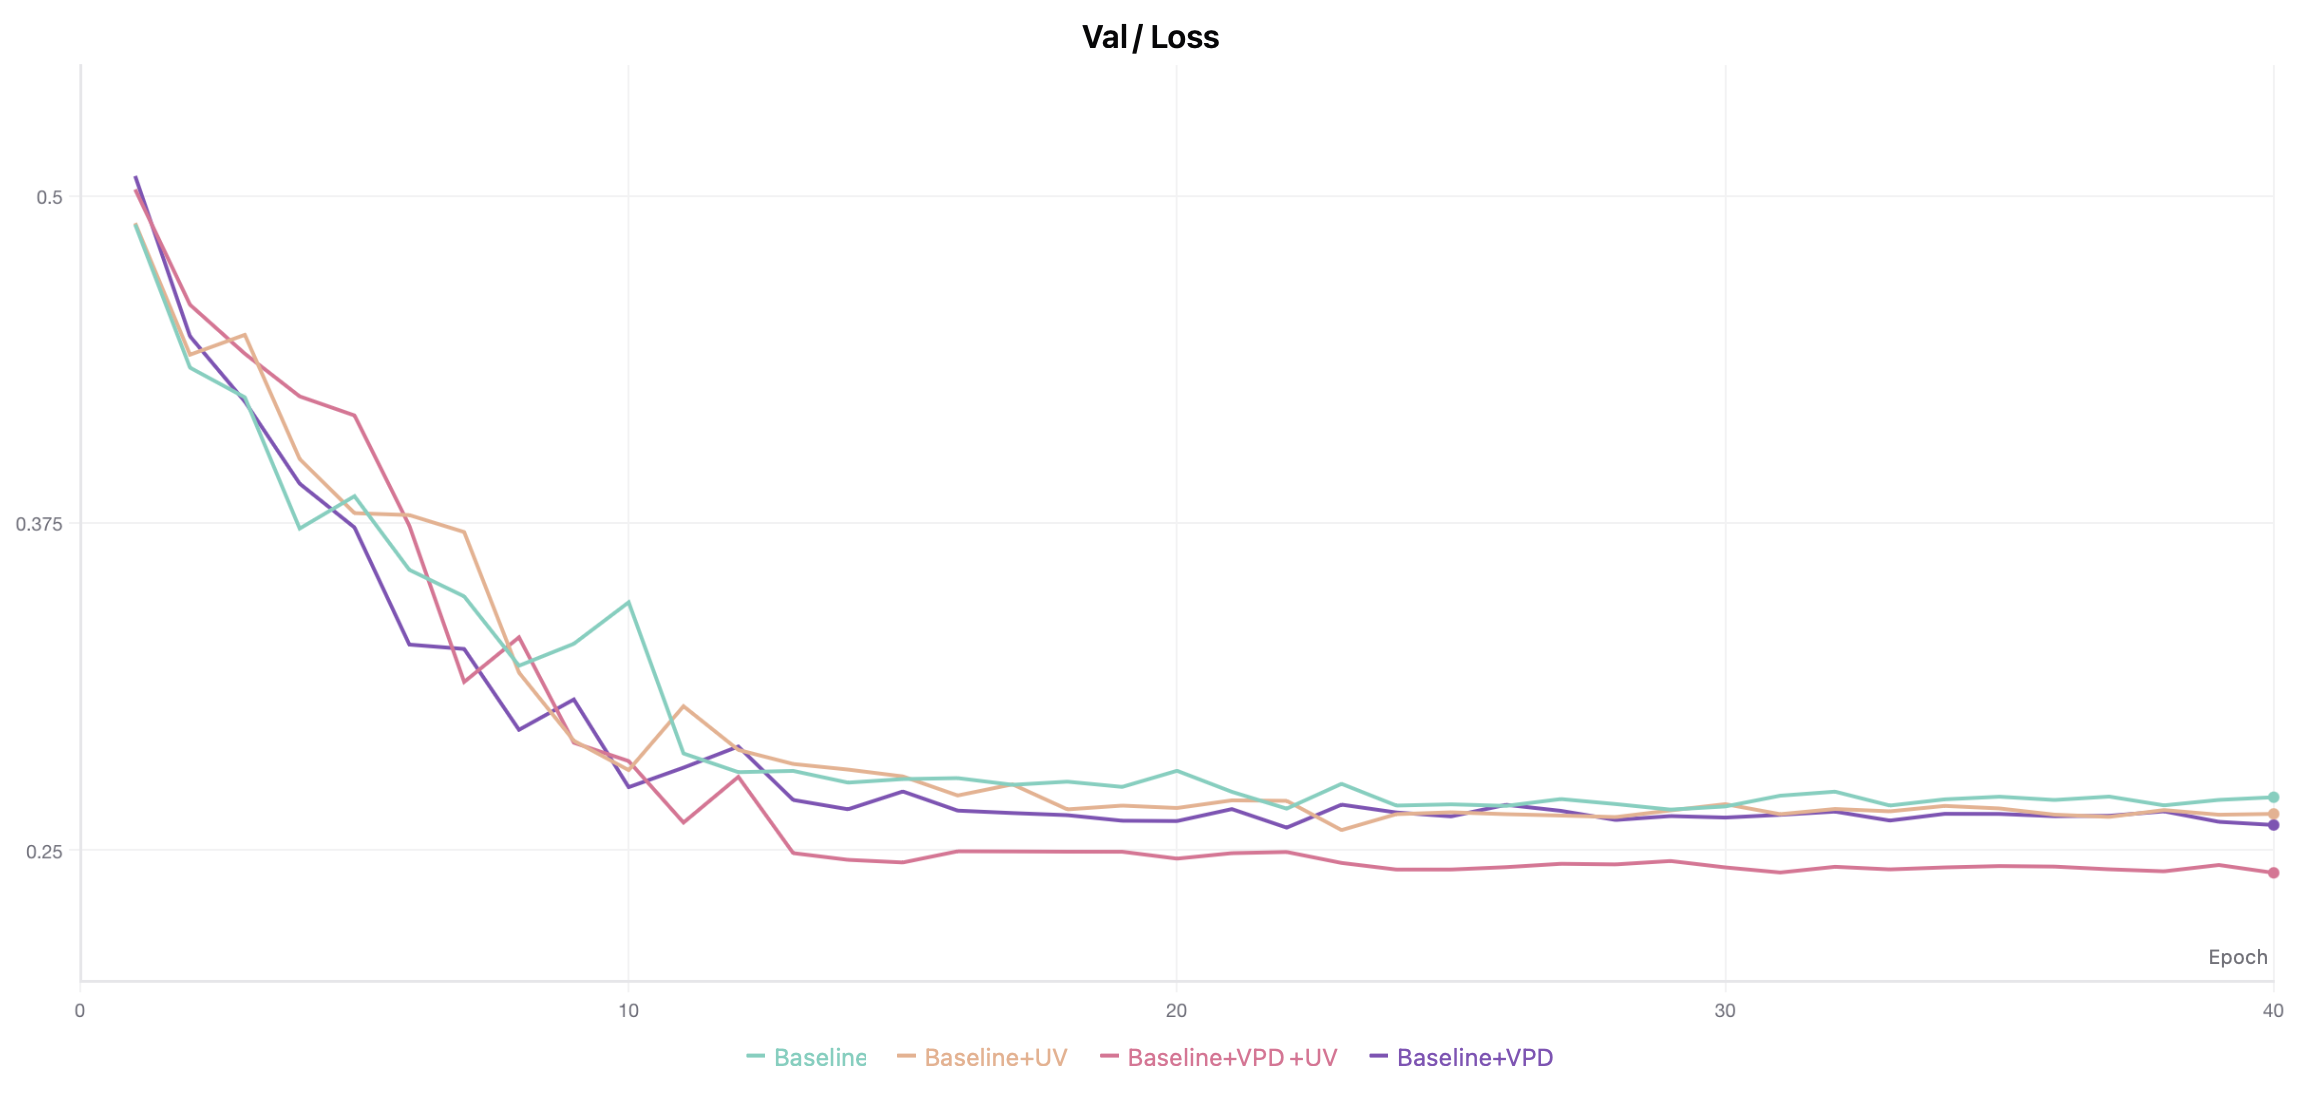
\includegraphics[width=\linewidth]{img/chap4/4-2-val-loss.png} 
        \centerline{(b) 验证集 Precision 曲线}
    \end{minipage}
    \caption{模型训练过程中的Precision曲线}
    \label{fig:4-2-train_val_precision}
\end{figure}

\section{总体预测性能对比}
\label{sec:4-3}
如表 \ref{tab:4-3-performance_comparison} 所示，本节在测试集上全面评估了模型（2D/3D Swin Transformer）与当前主流深度学习时空预测模型（LSTM, ConvLSTM, TimeSformer, 3D CNN）的定量性能。总体而言，本研究提出的融合物理信息的2D/3D Swin Transformer在总体准确率（OA）、精确率（Precision）、召回率（Recall）和核心指标 F1-Score 上均取得了全场最优表现。
\begin{table}[htbp]
    \centering
    \caption{不同深度学习模型在测试集上的定量结果，分类指标以百分比（\%）表示。}
    \label{tab:4-3-performance_comparison}
    \renewcommand{\arraystretch}{1.3} % 增加行高，提升阅读体验
    \resizebox{\textwidth}{!}{
        \begin{tabular}{lcccccc}
            \toprule
            \textbf{Algorithm} & \textbf{Config} & \textbf{Precision (↑)} & \textbf{Recall (↑)} & \textbf{F1-score (↑)} & \textbf{AUROC (↑)} & \textbf{OA (↑)} \\
            \midrule
            LSTM \cite{kondylatos2022wildfire} & -- & 73.74 & 82.17 & 77.72 & 96.53 & 93.80 \\
            ConvLSTM \cite{kondylatos2022wildfire} & -- & 82.40 & 76.75 & 79.47 & 97.12 & 94.78 \\
            TimeSformer \cite{bertasius2021space} & -- & 81.13 & 76.82 & 78.92 & 96.57 & 94.60 \\
            3D CNN \cite{loan} & -- & 82.72 & 80.98 & 81.72 & \textbf{97.15} & 95.23 \\
            \midrule
            \multirow{4}{*}{\makecell[c]{\textbf{2D/3D}\\\textbf{Swin Transformer}}}
            & Baseline & 82.41 & 82.75 & 82.58 & 96.68 & 95.41 \\
            & + VPD & 83.38 & 82.34 & 82.86 & 96.87 & 95.52 \\
            & + UV & 82.64 & \textbf{84.58} & 83.60 & 96.78 & 95.63 \\
            & + VPD + UV & \textbf{84.55} & 84.49 & \textbf{84.52} & 96.98 & \textbf{95.93} \\
            \bottomrule
        \end{tabular}
    }
\end{table}

观察基线模型数据可知，基于纯时间序列的 LSTM 模型虽然在召回率（82.17\%）上表现尚可，但其精确率仅为 73.74\%，且 F1-Score 垫底（77.72\%）。这表明缺乏空间维度交互的模型会产生大量误报。引入空间卷积的 ConvLSTM 与引入时间注意力的 TimeSformer 在精确率上有所改善，但召回率出现明显下滑。相比之下，本研究的 2D/3D Swin Transformer（Baseline）尚未引入任何物理先验，便已取得了 82.58\% 的 F1-Score，超越了所有序列和纯卷积模型。这充分证明了 Swin Transformer 的三维滑动窗口机制在捕捉火灾风险长距离时空依赖关系上的架构优越性。

在基线模型的基础上，不同物理先验信息的引入对模型性能产生了极具指向性的增益。
一方面，引入饱和水汽压差（+ VPD）后，模型的精确率（Precision）从 82.41\% 提升至 83.38\%。这从侧面印证了热力学特征重构的作用，饱和水汽压差比单纯的相对湿度更敏锐地刻画地表植被的异常脱水状态，降低了误报率。另一方面，引入风场动力学偏置（+ UV）后，模型在召回率（Recall）上实现了全场最高的 84.58\%。在野火防灾业务中，漏报的代价往往是灾难性的。风向信息的注入成功引导了模型的空间注意力向高危的下风向区域倾斜，增强了模型捕捉起火信号的能力。最终的模型（+ VPD + UV）实现了两者优势的叠加，F1-Score 达到 84.52\% 的峰值。因此，不同深度学习模型在测试集上的定量结果证明了本研究所提出模型的有效性。


    \chapter{可解释性分析}
\label{chap:5}

\section{基于SHAP的归因分析}
为了对深度神经网络在野火预测任务中的特性进行可解释性分析，本研究引入了基于博弈论理论的 SHAP（SHapley Additive exPlanations）解释框架。SHAP 的核心逻辑在于将模型对起火概率的预测视为一场由多种时空特征共同参与的“合作博弈” 。通过计算每个特征在所有可能的特征组合中带来的边际贡献，SHAP 能够为每一个输入变量分配一个量化的贡献值，即 SHAP 值。  
在数学表达上，SHAP 属于加性特征归因方法。对于一个特定的输入样本，其模型预测输出 $f(x)$ 可以表示为基线值（全体样本预测均值）与各个特征贡献值的线性累加：
\begin{equation}
     f(x) = \phi_0 + \sum_{i=1}^{M} \phi_i 
\end{equation}
其中，$\phi_0$ 为模型在无特征输入时的基础期望，$\phi_i$ 为第 $i$ 个特征的 SHAP 值。对于单个特征 $i$ 的 Shapley 值 $\phi_i$，其严格的理论计算公式如下：
\begin{equation}
    \phi_i = \sum_{S \subseteq F \setminus \{i\}} \frac{|S|!(|F| - |S| - 1)!}{|F|!} [f_{S \cup \{i\}}(x_{S \cup \{i\}}) - f_S(x_S)] 
\end{equation}

此处，$F$ 代表全体特征集合，$S$ 是不包含特征 $i$ 的任一特征子集。该公式通过对所有可能的特征排列顺序进行加权平均，确保了归因结果具备局部准确性、缺失性和一致性等优良数学性质。
SHAP（SHapley Additive exPlanations）是一种基于博弈论（Game Theory）中 Shapley 值的机器学习模型解释方法。其核心思想是将模型在特定样本上的预测结果视为各个输入特征（如气象、地貌、植被等）共同参与的一场“合作博弈”。模型最终的预测值与全体样本平均预测值（基线值）之间的偏差，被公平地分配给每个输入特征，这个分配值即为该特征的 SHAP 值。

在深度学习任务中，考虑到本研究所采用的 DualBranchSwinGCA 模型集成了 3D 滑动窗口注意力机制与地理感知交叉注意力（Geo-CA）模块，其内部梯度路径具有高度的非线性与复杂性。DeepSHAP 方法在处理此类自定义算子时容易出现算子不支持或梯度断裂的问题。因此，本实验采用了更为稳健的 GradientExplainer 解释器。该方法基于预期梯度（Expected Gradients）理论，通过在背景样本（Background Samples）和待解释样本之间进行路径积分，能够更稳健地分解模型在时空多模态输入下的预测逻辑。

在具体实施过程中，本研究首先筛选了 20 个未着火的负样本构建背景基线，用以代表环境的期望。由于模型输入包含地理坐标等非计算类元数据，本实验设计了一个模型包装器（Wrapper），将不参与特征提取的变量进行屏蔽，从而确保 SHAP 解释器能够聚焦于真正驱动火灾蔓延的特征变量。针对待解释的火灾正样本，本实验选取了 30 个具有代表性的真实火灾样本进行分批归因计算，通过在输入空间与背景空间之间进行路径梯度积分，计算出各要素的边际贡献,并取其 SHAP 绝对值的均值 $mean(\|SHAP\|)$ 作为衡量特征全局重要性的核心指标。为了清晰地展示不同维度特征的贡献，我们将输入特征划分为动态气象特征、静态地理特征以及地表覆盖类型特征（CLC），得到的全局变量贡献度排序如图 \ref{fig:5-1-shap} 所示。

\begin{figure}[htbp]
    \centering
    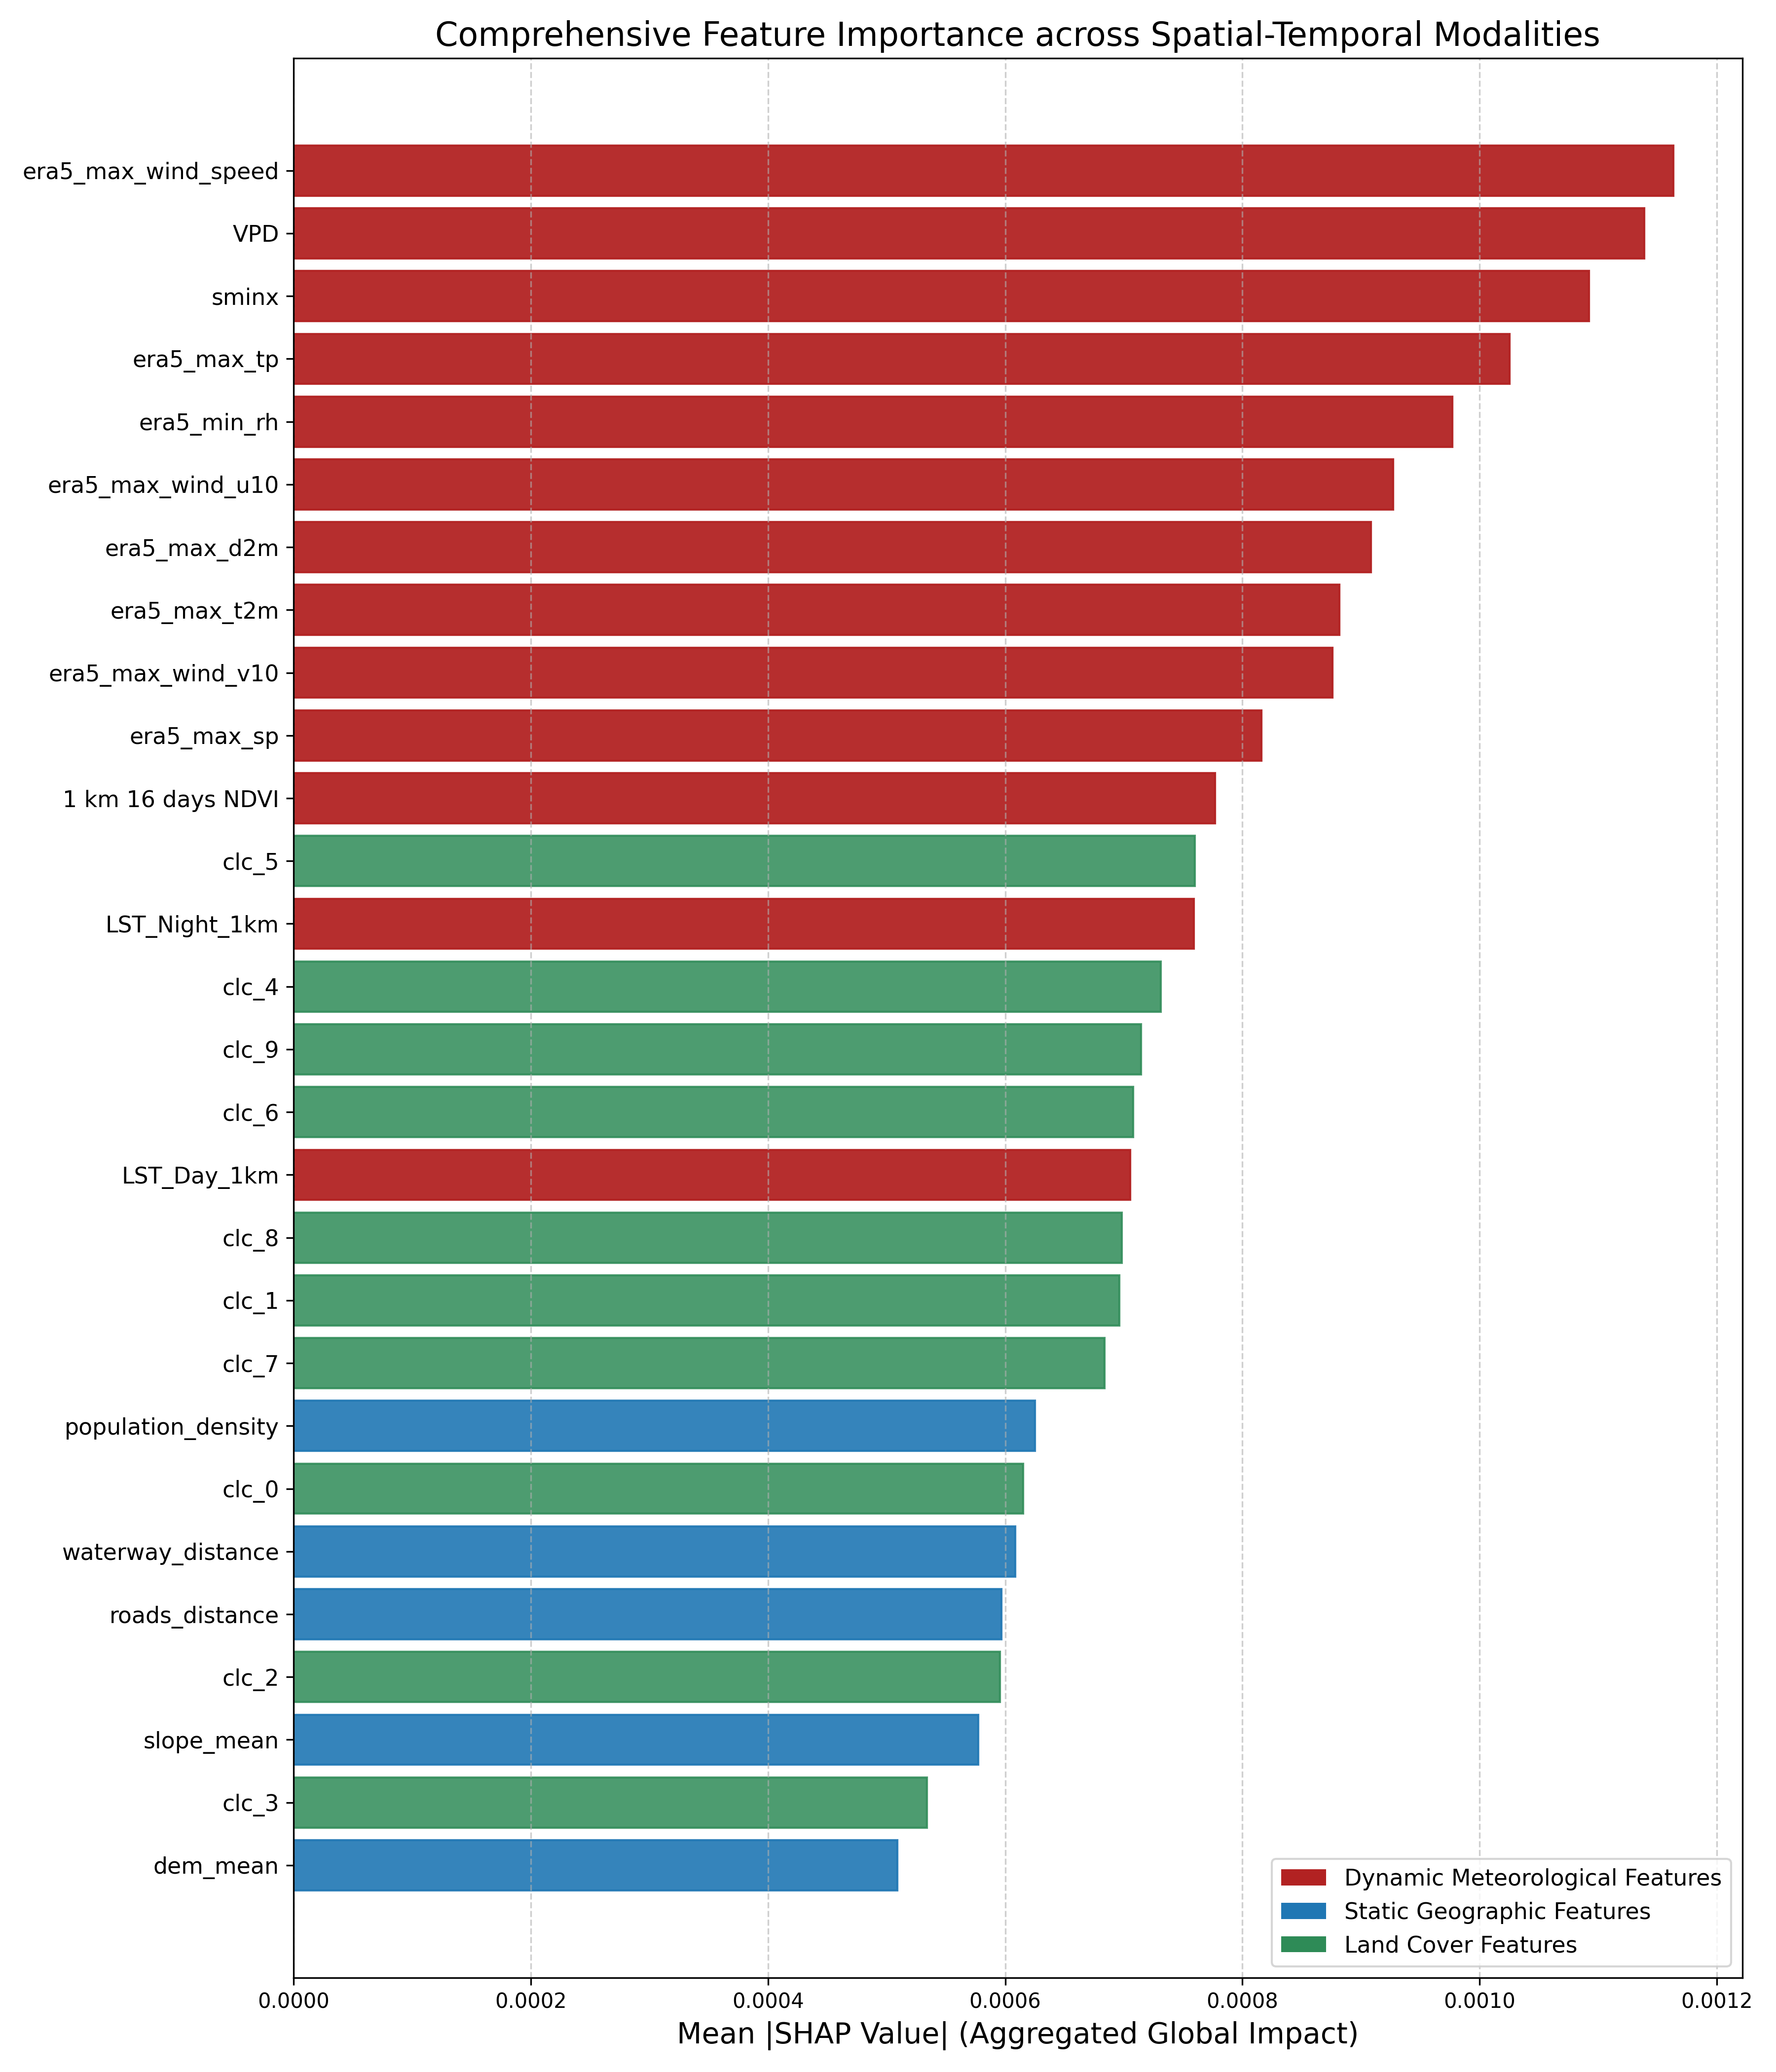
\includegraphics[width=0.9\textwidth]{img/chap5/5-1-shap-all.png}
    \caption{特征变量的SHAP值排序}
    \label{fig:5-1-shap}
\end{figure}

实验结果表明，动态气象特征在模型预测过程中起主导作用。其中，最大风速（$era5_max_wind_speed$）的特征重要性最高，而风场的两个分量 $wind_u10$ 与 $wind_v10$ 同样具有较高贡献。这说明风场信息对野火蔓延方向与传播速度具有显著影响，也从侧面验证了本文引入风场动力学偏置机制的合理性。此外，本文构建的饱和水汽压差（VPD）特征也表现出较高的重要性，其贡献高于传统的相对湿度与气温变量。这表明，相较于单一气象指标，VPD 能够更有效地反映空气干燥程度，以及可燃物失水状态，从而帮助模型更准确地识别高火险环境。

与动态特征相比，静态地理特征如海拔（$dem\_mean$）和坡度（$slope\_mean$）对预测结果的贡献相对较小。在土地覆盖特征方面，不同类别的植被类型展现了差异化的贡献度。总体上牧场和普通农用地的SHAP特征值较大，模型在计算时赋予了这些区域更高的权重。

\section{对于特征融合模块Geo-CA的空间交叉注意力分析}
本小节旨在探究地理感知交叉注意力（Geo-CA）模块是否能对动态变量和静态变量双分支进行融合，并基于风向矢量这一动力学特征进行偏置。故本节针对较大风速条件下的火灾样本，进行了空间注意力的提取与可视化分析。

具体提取与可视化方法如下，选取待预测的中心目标网格作为注意力计算的 Query，将周围的广阔空间上下文作为 Keys。通过截获模型前向传播过程中的 $saved_attn_weights$，提取出该中心网格对周围所有区域的注意力分配权重矩阵。由于经过网络的多层下采样，提取出的注意力图尺度为 $7\times 7$。为了与真实的物理空间对齐并便于可视化，本研究采用双三次插值（Bicubic Interpolation）算法，将其平滑上采样还原至原始的$25\times 25$空间分辨率，并进行 Min-Max 归一化处理。

\begin{figure}[htbp]
    \centering
    \begin{minipage}{0.45\textwidth}
        \centering
        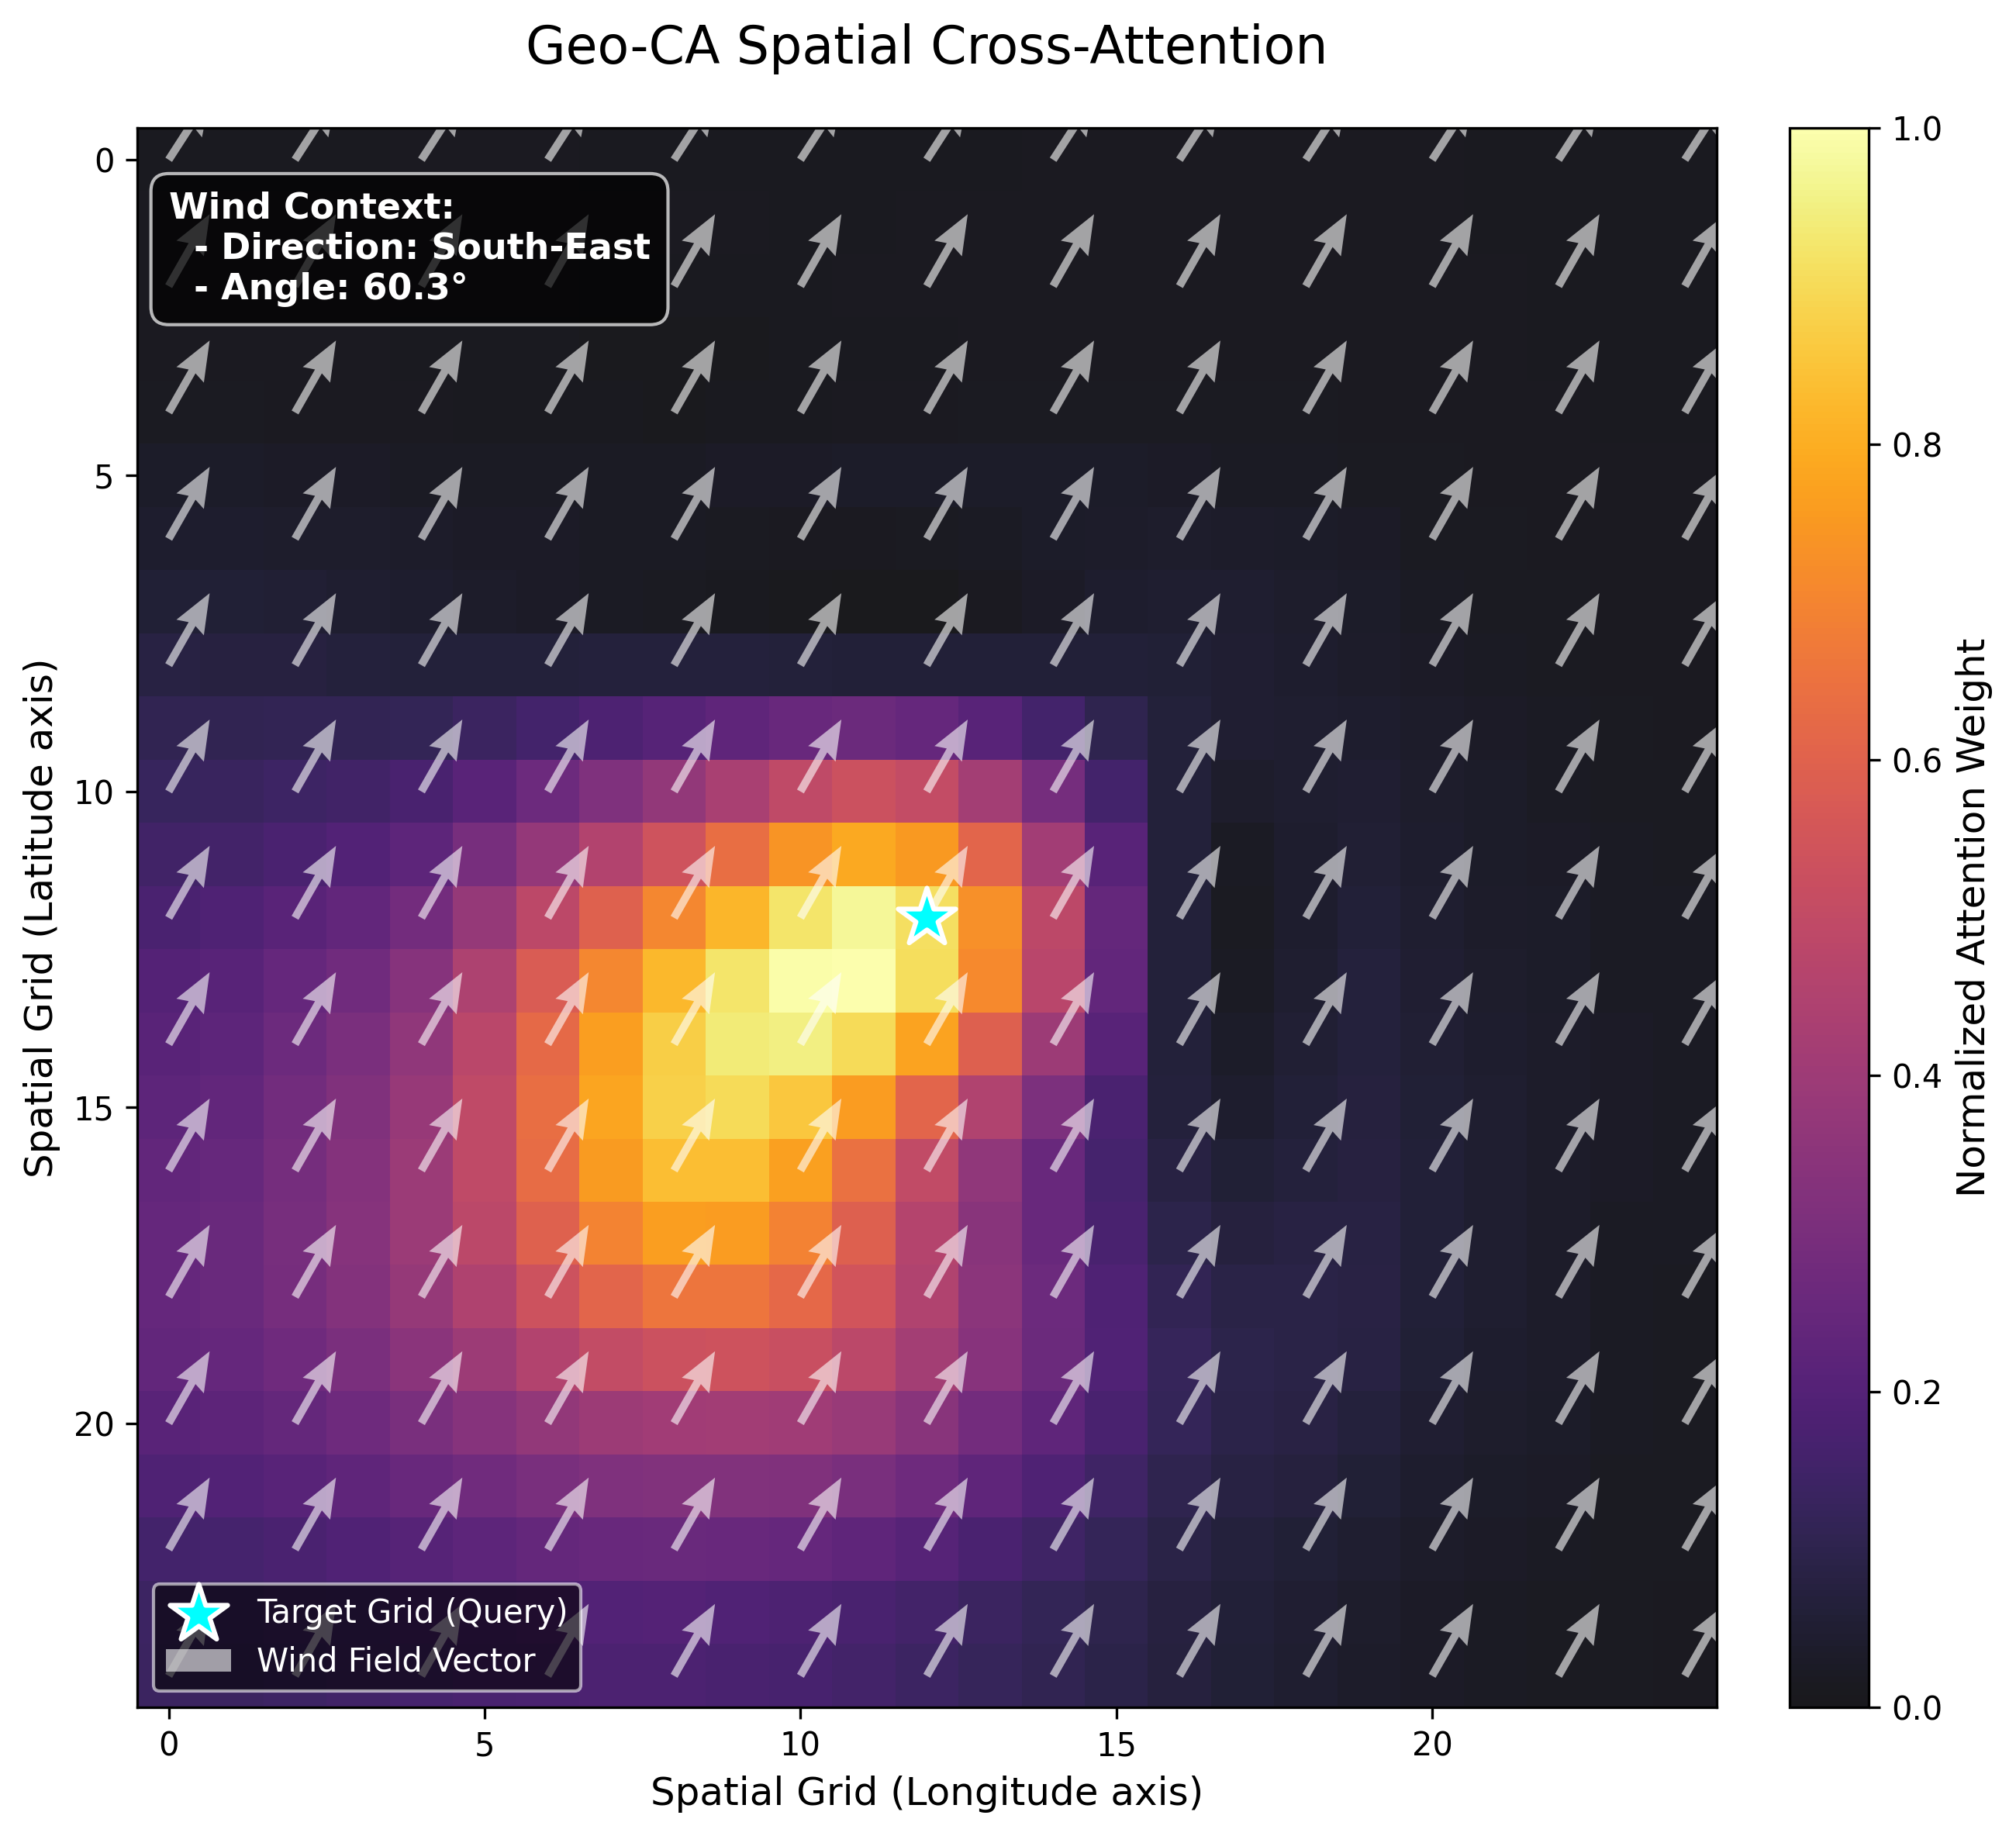
\includegraphics[width=\linewidth]{img/chap5/5-2-wind-attention-1.png} 
        \centerline{(a) 西南风，风速较大}
    \end{minipage}\hfill
    \begin{minipage}{0.45\textwidth}
        \centering
        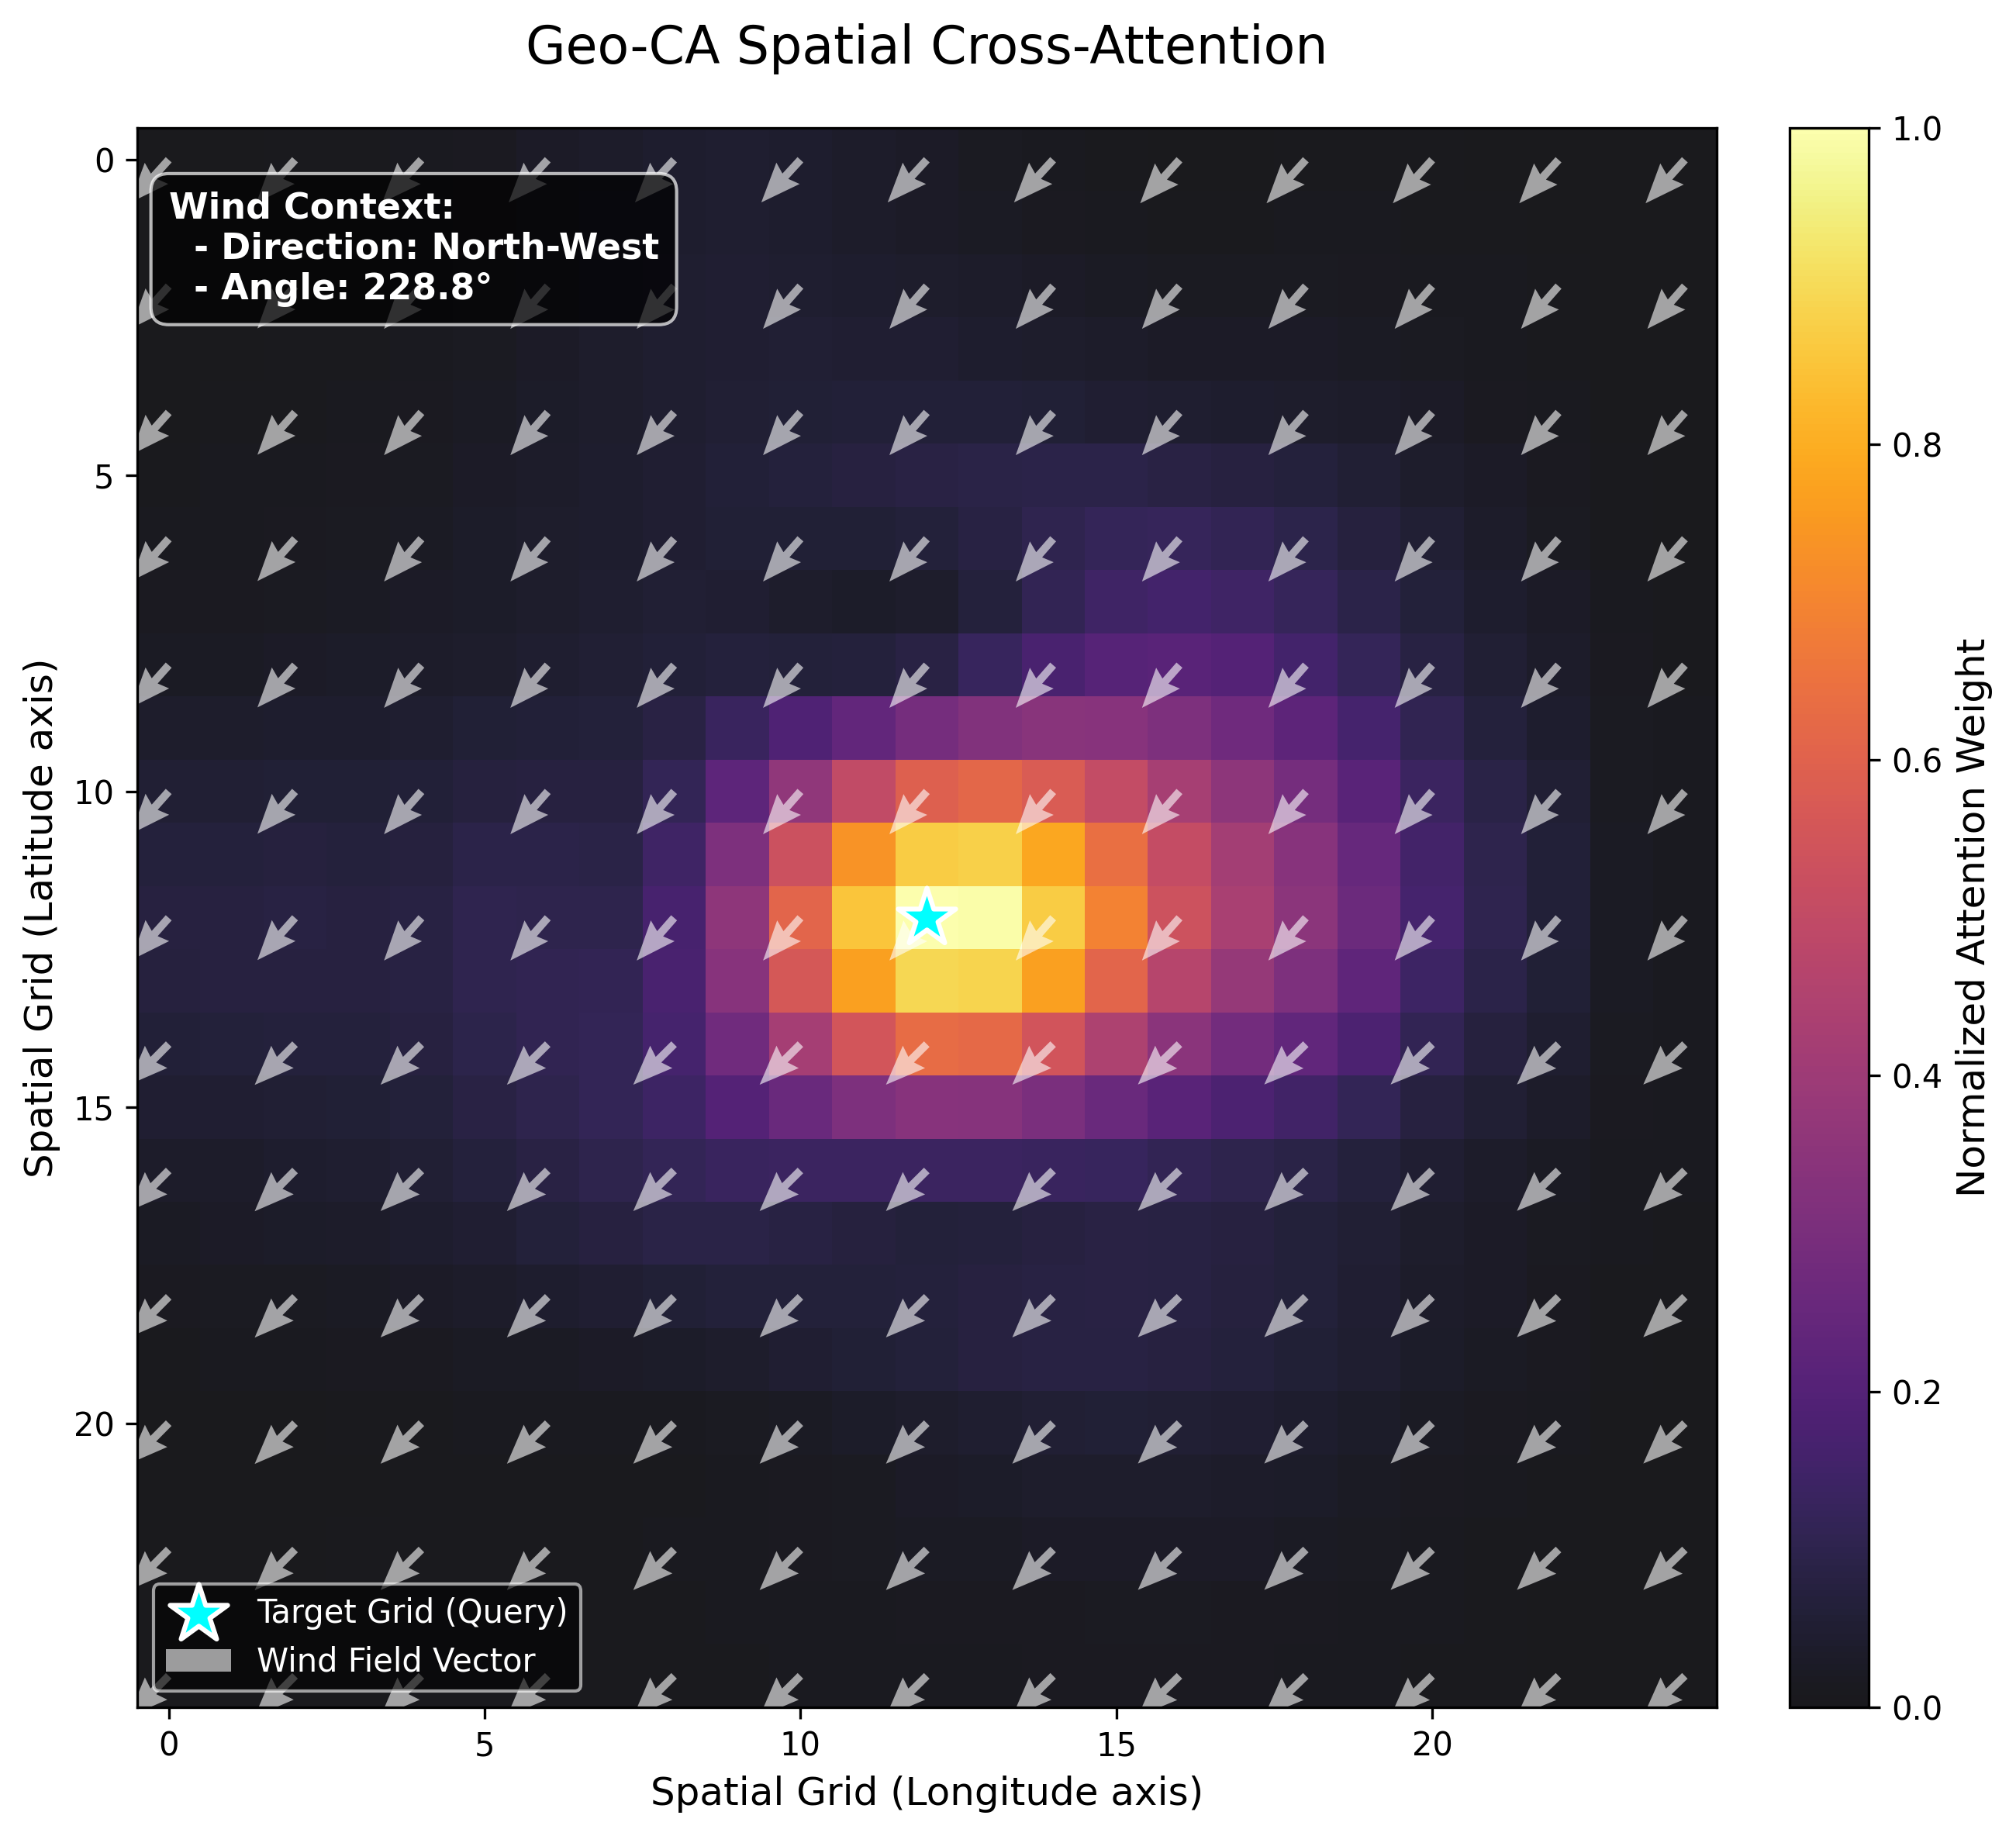
\includegraphics[width=\linewidth]{img/chap5/5-2-wind-attention-2.png} 
        \centerline{(b) 东北风，风速较小}
    \end{minipage}
    \caption{风场矢量对Geo-CA的空间注意力权重的影响}
    \label{fig:5-2-wind-attention}
\end{figure}

图\ref{fig:5-2-wind-attention}展示了风场矢量对Geo-CA的空间注意力权重的影响。图中箭头代表风场矢量，即箭头的方向代表风速的方向，箭头的长短代表风速的大小。对比(a)(b)两图可以看出，图(a)处于高风速环境，而图(b)处于低风速环境。对比两者的底层热力图可以发现：在风速较大的图(a)中，模型的高亮注意力区域明显向外扩散，呈现出更大的空间感受野；而在风速较小的图(b)中，注意力权重则较收敛、集中在预测中心点附近。此外，风向也影响了注意力权重的空间偏移。如对比图所示，注意力高度集中的高亮区域并非随机分布，而是与风向矢量的轴线存在显著的重合。更为关键的是，模型赋予了风的来向（即上风向区域）更大的注意力权重。

上述分析证明了风向矢量融入Geo-CA模块的有效性，Geo-CA 模块并非单纯的数学注意力映射，而能够根据风场矢量等物理特征进行注意力的偏置，从而为野火蔓延的预测注入物理学信息。

类似地，提取模型在 Geo-CA 融合前后的特征激活图（Feature Activation Maps）并进行可视化对比，图\ref{fig:5-2-branch-attention}分别展现了模型的静态特征激活图、动态特征激活图及融合后的最终激活状态的一个例子。观察可知，融合后的注意力区域并非左图与中图的简单线性叠加，而是同时捕获了静态与动态特征图的关键特征，证明了Geo-CA融合机制的有效性，也证明了双分支Swin Transformer结构的高效性。
\begin{figure}[htbp]
    \centering
    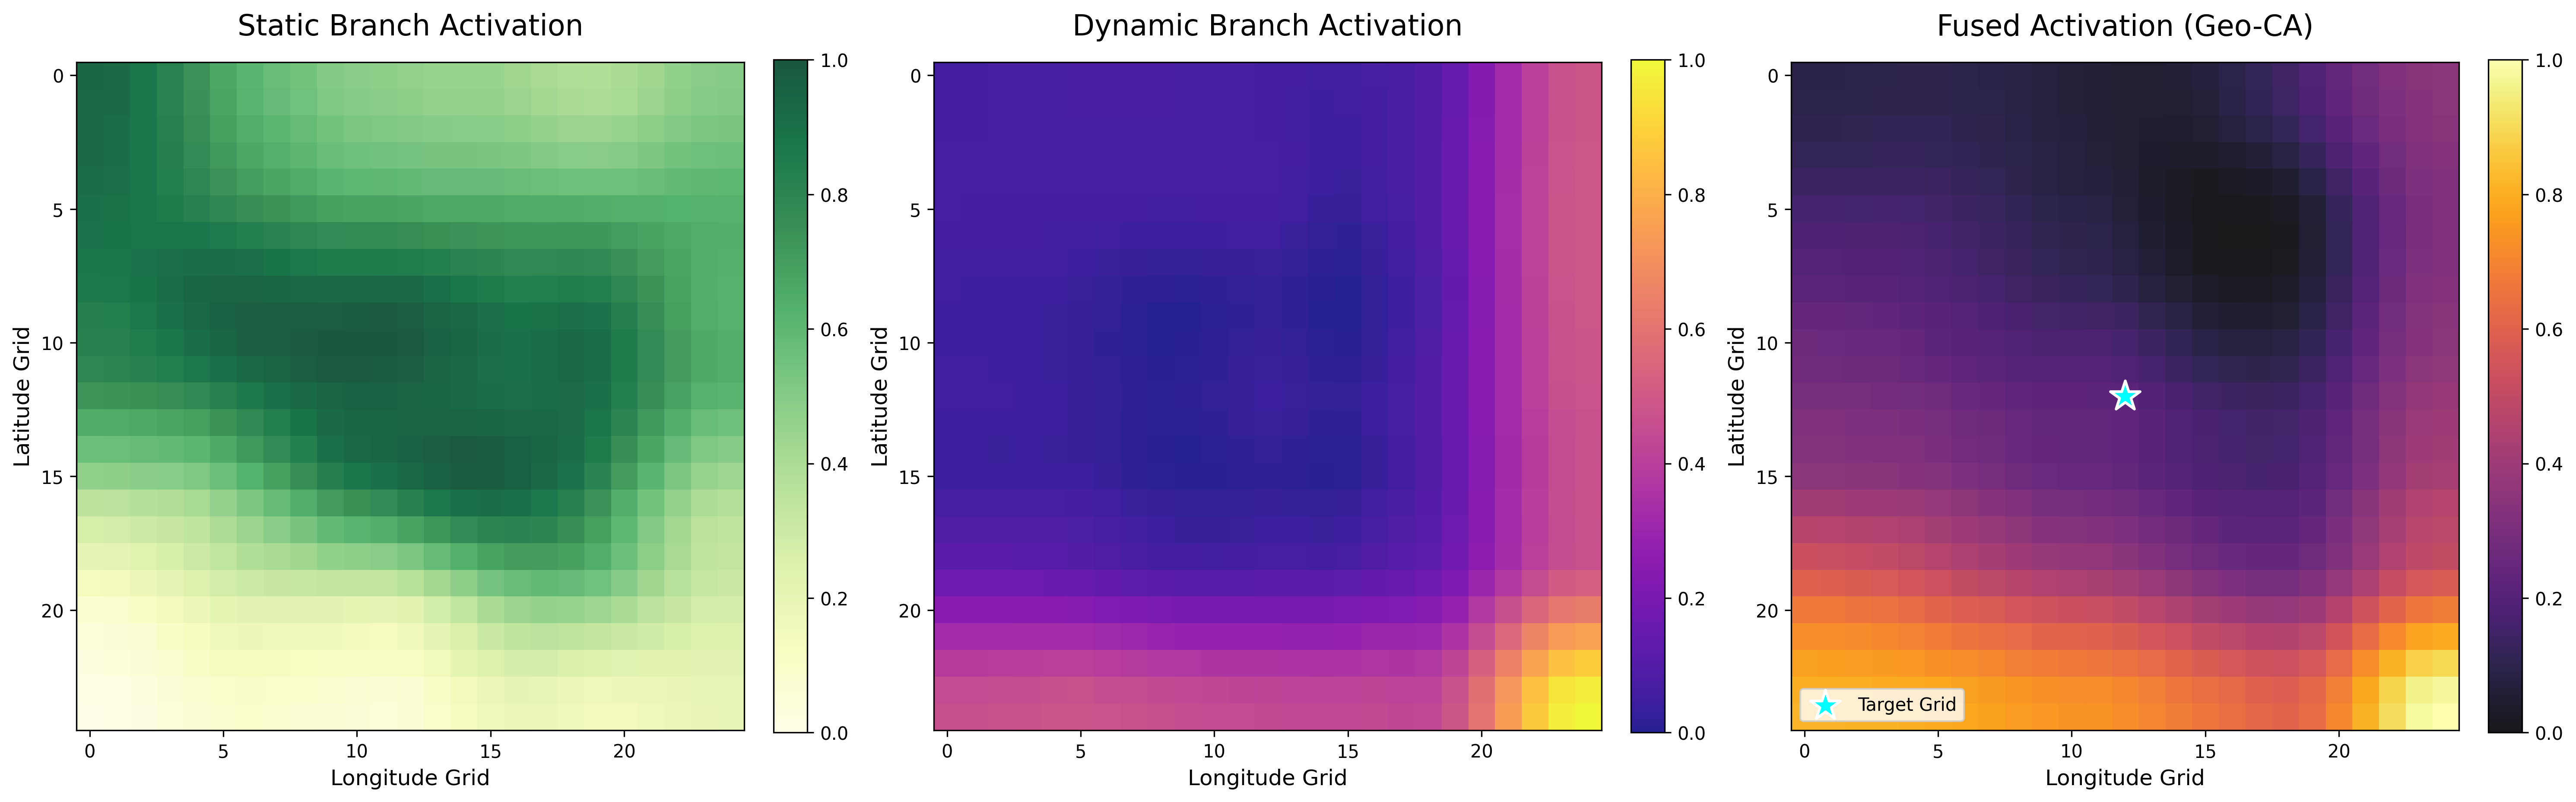
\includegraphics[width=0.9\textwidth]{img/chap5/5-2-branch-attention-1.png}
    \caption{Geo-CA 融合前后的特征激活图}
    \label{fig:5-2-branch-attention}
\end{figure}

本章针对深度学习模型的内部机制，进行了对本研究模型的可解释性分析。首先，利用基于博弈论的 SHAP 方法，探究了不同特征变量对野火预测的贡献程度。归因结果表明，最大风速和本研究引入的饱和水汽压差（VPD）等动态变量在野火预测中起到了主导作用，且不同土地覆盖类型呈现出差异化贡献，证明模型准确学习到了野火演化的核心动力学与热力学机制。其次，针对地理感知交叉注意力（Geo-CA）模块进行了可视化探究。通过对比不同风速与风向条件下的注意力分布，发现其能够打破各向同性的空间注意力计算限制，对风向矢量偏置做出注意力响应。特征激活图对比则展现了双分支结构的解耦提取能力，以及 Geo-CA 作为融合机制的精准有效。综合上述分析，验证了本研究提出的模型架构具备科学合理性与物理可解释性。
    \chapter{总结与讨论}
\label{chap:conclusion}

\section{总结}

本研究利用希腊及地中海地区的 FireCube 多变量时空数据集，进行野火风险预测的研究。首先介绍FireCube数据集的区域概况及时空数据构建，采样方式及训练数据，并详细分析其特征变量，为模型的构建奠定基础。

模型采用时空解耦的双分支架构：利用 3D Swin Transformer 分支通过三维滑动窗口机制提取气象序列的时空演化特征；利用 2D Swin Transformer 分支编码地形、植被等静态地理背景先验。在特征融合阶段，设计了地理感知交叉注意力机制（Geo-CA）。为弥补数据驱动模型在物理感知上的局限，本研究创新性地采用物理启发式特征重构。通过克劳修斯-克拉珀龙方程推导并利用马格努斯-泰登经验公式，将原始气温与露点温度变量重构为饱和水汽压差（VPD），用以定量刻画大气环境的潜在蒸发需求与植被燃料的脱水压力。此外，模型通过对 U（经向）和 V（纬向）风速分量的物理还原，得到风场矢量，并通过计算局部风场矢量与空间相对向量的点积，将风场动力学偏置硬编码至注意力权重计算中。这一设计打破了标准注意力机制的各向同性局限，使模型能够感知风场信息。

实验结果表明，该模型在测试集上的 F1-Score 达到 84.52\%，显著优于 LSTM、ConvLSTM 等主流基准模型。消融实验证实，饱和水汽压差VPD的特征重构有效降低了误报率，而风场偏置注入则显著提升了对下风向危险信号的捕捉能力（召回率达 84.58\%）。最后，通过 SHAP 归因分析验证了最大风速与 VPD 的对野火概率预测的突出贡献地位，并结合空间交叉注意力图的可视化，直观展示了注意力分布随物理风场偏移的规律，证实了模型决策逻辑与林火空气动力学常识的高度一致性。

\section{局限性及未来展望}

本研究虽然在融合物理信息的野火预测方面取得了一定进展，但仍存在若干局限性。首先，在数据表征维度上，目前输入的特征变量尚不充足，缺乏如火势历史动态轨迹等关键物理过程特征，且土地覆盖分类的粒度仍有提升空间，难以捕捉微观尺度的燃料结构差异。受限于原始数据集的分辨率，本研究采用的1km$\times$1km空间尺度在处理地形剧烈波动或城乡交界处的精细化蔓延时仍显粗糙。其次，本实验主要聚焦于地中海气候下的希腊地区，由于全球不同地区的火灾驱动机制存在区别，模型在跨气候带的大规模泛化能力及在全球范围内的训练样本储备仍需进一步加强。此外，受计算资源及样本规模限制，当前双分支网络的深度配置较为克制，在提取深层高阶物理演化语义方面可能存在表征瓶颈。

展望未来，研究工作将重点从以下几个方向展开。一是多源高分辨率数据的深度集成，通过引入遥感影像数据及具备穿透能力的雷达数据，提升模型对复杂环境的感知精度。二是探索全球化的预训练与迁移学习范式，利用海量多区域数据进行自监督学习，以克服单一区域正样本不足的局限性。三是进一步深化物理信息与深度学习架构的耦合，尝试将更为复杂的野火蔓延方程以算子学习或损失函数约束的形式嵌入更深层的模型架构中，旨在构建参数容量更大、物理一致性更强且具备全球预测能力的野火风险预测大模型。
    
    \appendix
    % chap/app.tex

\chapter{模型核心模块代码实现}
\label{appendix:A}

本附录提供了本文提出的时空解耦双分支 Swin Transformer预测模型的核心代码实现，基于 PyTorch 深度学习框架编写。

\section{动态气象分支与静态地形分支算法实现}
\label{app:A-1}
此处展示模型中用于处理动态变量的 \texttt{DynamicSwin3D} 模块，
% 第一个代码框：动态分支
\lstinputlisting[language=Python, caption=动态变量提取模块 (DynamicSwin3D) 实现]{code/DynamicSwin3D.py}

此处展示模型中用于处理静态变量的 \texttt{StaticSwin2D} 模块。

% 第二个代码框：静态分支
\lstinputlisting[language=Python, caption=静态变量编码模块 (StaticSwin2D) 实现]{code/StaticSwin2D.py}
\section{地理感知交叉注意力机制融合模块算法实现}
\label{app:A-2}
此处展示模型中的地理感知交叉注意力机制\texttt{GeoCrossAttention}融合模块。
\lstinputlisting[language=Python, caption=地理感知交叉注意力模块 (GeoCrossAttention) 实现]{code/GeoCrossAttention.py}



    
    \fancyempty
    \renewcommand{\bibname}{参考文献}
    \printbibliography[heading = bibintoc]

    \backmatter
    \chapter{致谢}
在写毕业论文之前，心心念念要写致谢感慨一番，而真正写完了却提不起力气再写致谢，或是回顾这四年。有些轻舟已过万重山之感吧，无疑是我人生目前为止最重要的四年，在这里我不断成长，真正成人。

毕业论文终稿截止的那天正好是我的22岁生日，也是我写下致谢时，再向后推十小时。18岁生日时赶上成人礼，我在盘锦高中的教室里吃着蛋糕，焦虑着十天后的高考，也憧憬着大学生活。四年后的今天我坐在北京大学图书馆，在三楼东区我最熟悉的区域，窗外天阴阴的，下了点小雨，我依然焦虑未来，但我想我有了更多底气。

感谢自己，能够诚实地面对自己的感受，保持困惑地思考。感谢在最艰难的时候，也许是大一大二迷茫时，也许是大三保研时，没有放弃自己，越来越相信自己。有勇气尝试，探索更广阔的世界，再不断回到脚下前行。希望自己能不断变好，但我愿做我最忠诚的朋友。我有时感叹，自己对自己负责是最难的事情，但四年里我慢慢学会了这件事。

感谢我的父母，感谢你们永远相信我，不给我压力，鼓励和安慰一直陪伴着我，你们是最棒的父母，温暖的家永远是庇护。

感谢我的朋友们，和你们在一起永远是最开心的。生活有时候很难，看着你们也在认真过，追求想要的东西，为你们高兴，也不断鼓舞着我。喜欢与你们吃饭，闲聊，在湖边散步。

感谢一路上遇到的老师，师长，同学，你们在不同时刻给我激励，让我看到另一种可能，从你们的身上我学到很多。感谢我的导师陈语谦老师，谢谢您的认可，让我幸运地得以在深研院度过未来三年；感谢连宙辉老师，虽然和您交流不多，但第一次的科研经历让我更加坚定；感谢我的毕业论文导师俞妍老师，您的鼓励总是那么真诚，这份鼓励也会继续让我前行。在提到这些时，我总是想说，谢谢你们“收留”我，在面对并不光鲜的履历时，你们给了我机会，也许有些我最终完成得也不尽如人意，但我尝试过也努力过。谢谢一路上遇到的师长，成鹏师兄，昱博师兄，一鸣师兄，林杭师兄，宇轩师兄，模仿是最好的学习方式，我不断从你们身上汲取着能量，从零开始学会做科研，学会与人合作。感谢丰楗师兄对本毕业论文的大力支持。

感谢物理学院，虽然本科的物理课程我吸收得并不好，但学院大部分时候都让我很舒服。

感谢北大，你是最宽容的。慢慢地我发现，其实是大一第一个月我就发现，我还挺适合这里的，作为一个普通人，北大给了我无需被评判的普通的自由。喜欢园子里的草木，喜欢从近邻宝到南门高高的树，喜欢从图书馆穿过燕南园到家园食堂，喜欢图书馆三楼东区，西区301和里面的小仓库，一楼新书展阅厅，和声厅，喜欢二教207和208，三楼靠窗的自习区，喜欢理教三四楼的自习区，喜欢经院自习区，喜欢我的宿舍，33楼214和34A420，喜欢随机刷新的小猫，喜欢绕着未名湖走路，喜欢时常拥挤的理教健身房。四年过去了，我还是爱吃松林的包子，学一的襄阳牛肉面，农二的木桶饭，燕南的家常菜，家三的中式简餐，各处的麻辣香锅。习惯在闲得没事的时候去29楼和45楼地下溜达一圈，心情不好的时候去未名湖、或者从西门外走到圆明园。有时也感到压抑想要逃离，但每天晚上回来踏进校园的一刻，还是感到安心。

感谢电影，谢谢百讲，资料馆，法文，百老汇，谢谢北影节，爱酷，以及各种各样的电影活动，如果没有遇到和爱上电影我不知道会怎样。谢谢戴老师，谢谢因电影遇到的很多朋友们，能和你们相遇、一起聊天真的很幸福。大学四年“浪费时间”最多的事就是看电影了吧。喜欢/兴趣/爱好完全不需要理由，但某种程度上电影让我更加自洽。

感谢北京，你和北大一样包容，你有些破烂又无比宽广的胸襟让我见识到18岁时想要看到的世界。先是探索带来的新奇，后是厌倦，要毕业了又开始舍不得北京。不远的路我喜欢骑车，穿过街道看看两旁。我像拿着图钉标记地点，标记着那些景点，街道，小店，有些可能已经不在，但也钉在了我的回忆地图里。能在北京不同地方看到不同的建筑，不同的风格，完全不同的人做各种各样的事，因为基数和范围足够大所以有趣的事也多，我也就在探索中慢慢了解了这座城市，也许有缘再会。

感谢互联网。

继续散步吧，继续前行吧。
    % \include{chap/origin}

\end{document}

% vim:ts=4:sw=4